
\documentclass[11pt,a4paper]{article}
\usepackage[T1]{fontenc}
\usepackage[utf8]{inputenc}
\usepackage{lmodern}
\usepackage[a4paper,margin=25mm]{geometry}
\usepackage{amsmath,amssymb,amsthm}
\usepackage{microtype}
\usepackage{graphicx,longtable,booktabs,array,calc,float}
\usepackage[font=small,labelfont=bf]{caption}
\usepackage[hidelinks,pdfencoding=auto]{hyperref}
\input{glyphtounicode}
\pdfgentounicode=1
\pdfsuppressptexinfo=15
\pdfinfoomitdate=1
\pdftrailerid{}
\pdfinfo{
/FontNotices <2320456d62656464656420666f6e74730a0a5468652061727469636c6520656d626564732073756273657473206f66204c6174696e204d6f6465726e2c20414d532073796d626f6c20666f6e747320616e642044656a6156752053616e730a616e642053657269662e205468652044656a615675207375627365747320636f6d652066726f6d2074686520766563746f7220696c6c757374726174696f6e732e0a54686520656d62656464656420666f6e742070726f6772616d73206361727279207468656972206f776e206c6963656e7365732e0a0a2d204c6174696e204d6f6465726e2c20627920422e204a61636b6f77736b6920616e64204a2e204d2e204e6f7761636b692c2075736573207468650a20205b4755535420466f6e74204c6963656e73655d286c6963656e7365732f475553542d464f4e542d4c4943454e53452e7478742920616e64207468650a20205b4c615465582050726f6a656374205075626c6963204c6963656e73655d286c6963656e7365732f4c50504c2d312e33632e747874292e0a2d20414d53466f6e74732061726520636f707972696768742028632920313939372c20323030392c20416d65726963616e204d617468656d61746963616c20536f63696574792e0a202053656520746865205b53494c204f70656e20466f6e74204c6963656e736520616e64206e6f74696365735d286c6963656e7365732f414d532d4f464c2d312e312e747874292e0a2d2044656a61567520696e636c756465732042697473747265616d205665726120616e642041726576206d6174657269616c2e205468650a20205b636f7079726967687420616e64206c6963656e7365206e6f74696365735d286c6963656e7365732f44656a6156752d636f707972696768742e747874290a202067697665207468652066756c6c207465726d73206f6620746865736520666f6e74732e0a>
/FontLicenseGUST <2520546869732069732076657273696f6e20312e302c206461746564203232204a756e6520323030392c206f6620746865204755535420466f6e74204c6963656e73652e0a252028475553542069732074686520506f6c697368205465582055736572732047726f75702c20687474703a2f2f7777772e677573742e6f72672e706c290a250a2520466f7220746865206d6f737420726563656e742076657273696f6e206f662074686973206c6963656e7365207365650a2520687474703a2f2f7777772e677573742e6f72672e706c2f666f6e74732f6c6963656e7365732f475553542d464f4e542d4c4943454e53452e7478740a25206f720a2520687474703a2f2f7475672e6f72672f666f6e74732f6c6963656e7365732f475553542d464f4e542d4c4943454e53452e7478740a250a25205468697320776f726b206d617920626520646973747269627574656420616e642f6f72206d6f64696669656420756e6465722074686520636f6e646974696f6e730a25206f6620746865204c615465582050726f6a656374205075626c6963204c6963656e73652c206569746865722076657273696f6e20312e3363206f6620746869730a25206c6963656e7365206f722028617420796f7572206f7074696f6e2920616e79206c617465722076657273696f6e2e0a250a2520506c6561736520616c736f206f6273657276652074686520666f6c6c6f77696e6720636c617573653a0a25203129206974206973207265717565737465642c20627574206e6f74206c6567616c6c792072657175697265642c2074686174206465726976656420776f726b732062650a25202020206469737472696275746564206f6e6c79206166746572206368616e67696e6720746865206e616d6573206f662074686520666f6e747320636f6d70726973696e6720746869730a2520202020776f726b20616e6420676976656e20696e20616e206163636f6d70616e79696e6720226d616e6966657374222c20616e642074686174207468650a252020202066696c657320636f6d70726973696e672074686520576f726b2c206173206c697374656420696e20746865206d616e69666573742c20616c736f20626520676976656e0a25202020206e6577206e616d65732e20416e7920657863657074696f6e7320746f207468697320726571756573742061726520616c736f20676976656e20696e207468650a25202020206d616e69666573742e0a250a25202020205765207265636f6d6d656e6420746865206d616e696665737420626520676976656e20696e20612073657061726174652066696c65206e616d65640a25202020204d414e49464553542d3c666f6e7469643e2e7478742c207768657265203c666f6e7469643e20697320736f6d6520756e69717565206964656e74696669636174696f6e0a25202020206f662074686520666f6e742066616d696c792e20496620612073657061726174652022726561646d65222066696c65206163636f6d70616e6965732074686520576f726b2c0a25202020207765207265636f6d6d656e642061206e616d65206f662074686520666f726d20524541444d452d3c666f6e7469643e2e7478742e0a250a2520546865206c61746573742076657273696f6e206f6620746865204c615465582050726f6a656374205075626c6963204c6963656e736520697320696e0a2520687474703a2f2f7777772e6c617465782d70726f6a6563742e6f72672f6c70706c2e74787420616e642076657273696f6e20312e3363206f72206c617465720a252069732070617274206f6620616c6c20646973747269627574696f6e73206f66204c615465582076657273696f6e20323030362f30352f3230206f72206c617465722e0a>
/FontLicenseLPPL <>
/FontLicenseAMS <>
/FontLicenseDejaVu <466f726d61743a2068747470733a2f2f7777772e64656269616e2e6f72672f646f632f7061636b6167696e672d6d616e75616c732f636f707972696768742d666f726d61742f312e302f0a557073747265616d2d4e616d653a2044656a61567520666f6e74730a557073747265616d2d417574686f723a2053746570616e20526f68203c7372634075736572732e736f75726365666f7267652e6e65743e20286f726967696e616c20617574686f72292c0a202020202020202020202020202020202020736565202f7573722f73686172652f646f632f666f6e74732d64656a6176752d636f72652f415554484f525320666f722066756c6c206c6973740a536f757263653a2068747470733a2f2f64656a6176752d666f6e74732e6769746875622e696f2f0a0a46696c65733a202a0a436f707972696768743a20436f707972696768742028632920323030332062792042697473747265616d2c20496e632e20416c6c205269676874732052657365727665642e200a2042697473747265616d205665726120697320612074726164656d61726b206f662042697473747265616d2c20496e632e0a2044656a615675206368616e6765732061726520696e207075626c696320646f6d61696e2e0a4c6963656e73653a2062697473747265616d2d766572610a205065726d697373696f6e20697320686572656279206772616e7465642c2066726565206f66206368617267652c20746f20616e7920706572736f6e206f627461696e696e67206120636f70790a206f662074686520666f6e7473206163636f6d70616e79696e672074686973206c6963656e7365202822466f6e7473222920616e64206173736f6369617465640a20646f63756d656e746174696f6e2066696c657320287468652022466f6e7420536f66747761726522292c20746f20726570726f6475636520616e642064697374726962757465207468650a20466f6e7420536f6674776172652c20696e636c7564696e6720776974686f7574206c696d69746174696f6e207468652072696768747320746f207573652c20636f70792c206d657267652c0a207075626c6973682c20646973747269627574652c20616e642f6f722073656c6c20636f70696573206f662074686520466f6e7420536f6674776172652c20616e6420746f207065726d69740a20706572736f6e7320746f2077686f6d2074686520466f6e7420536f667477617265206973206675726e697368656420746f20646f20736f2c207375626a65637420746f207468650a20666f6c6c6f77696e6720636f6e646974696f6e733a0a202e0a205468652061626f766520636f7079726967687420616e642074726164656d61726b206e6f746963657320616e642074686973207065726d697373696f6e206e6f74696365207368616c6c0a20626520696e636c7564656420696e20616c6c20636f70696573206f66206f6e65206f72206d6f7265206f662074686520466f6e7420536f667477617265207479706566616365732e0a202e0a2054686520466f6e7420536f667477617265206d6179206265206d6f6469666965642c20616c74657265642c206f7220616464656420746f2c20616e6420696e20706172746963756c61720a207468652064657369676e73206f6620676c79706873206f72206368617261637465727320696e2074686520466f6e7473206d6179206265206d6f64696669656420616e640a206164646974696f6e616c20676c79706873206f722063686172616374657273206d617920626520616464656420746f2074686520466f6e74732c206f6e6c792069662074686520666f6e74730a206172652072656e616d656420746f206e616d6573206e6f7420636f6e7461696e696e67206569746865722074686520776f726473202242697473747265616d22206f722074686520776f72640a202256657261222e0a202e0a2054686973204c6963656e7365206265636f6d6573206e756c6c20616e6420766f696420746f2074686520657874656e74206170706c696361626c6520746f20466f6e7473206f7220466f6e740a20536f667477617265207468617420686173206265656e206d6f64696669656420616e6420697320646973747269627574656420756e64657220746865202242697473747265616d0a205665726122206e616d65732e0a202e0a2054686520466f6e7420536f667477617265206d617920626520736f6c642061732070617274206f662061206c617267657220736f667477617265207061636b61676520627574206e6f0a20636f7079206f66206f6e65206f72206d6f7265206f662074686520466f6e7420536f66747761726520747970656661636573206d617920626520736f6c6420627920697473656c662e0a202e0a2054484520464f4e5420534f4654574152452049532050524f564944454420224153204953222c20574954484f55542057415252414e5459204f4620414e59204b494e442c20455850524553530a204f5220494d504c4945442c20494e434c5544494e4720425554204e4f54204c494d4954454420544f20414e592057415252414e54494553204f46204d45524348414e544142494c4954592c0a204649544e45535320464f52204120504152544943554c415220505552504f534520414e44204e4f4e494e4652494e47454d454e54204f4620434f505952494748542c20504154454e542c0a2054524144454d41524b2c204f52204f544845522052494748542e20494e204e4f204556454e54205348414c4c2042495453545245414d204f522054484520474e4f4d450a20464f554e444154494f4e204245204c4941424c4520464f5220414e5920434c41494d2c2044414d41474553204f52204f54484552204c494142494c4954592c20494e434c5544494e470a20414e592047454e4552414c2c205350454349414c2c20494e4449524543542c20494e434944454e54414c2c204f5220434f4e53455155454e5449414c2044414d414745532c0a205748455448455220494e20414e20414354494f4e204f4620434f4e54524143542c20544f5254204f52204f54484552574953452c2041524953494e472046524f4d2c204f5554204f460a2054484520555345204f5220494e4142494c49545920544f205553452054484520464f4e5420534f465457415245204f522046524f4d204f54484552204445414c494e475320494e205448450a20464f4e5420534f4654574152452e0a202e0a2045786365707420617320636f6e7461696e656420696e2074686973206e6f746963652c20746865206e616d6573206f6620476e6f6d652c2074686520476e6f6d650a20466f756e646174696f6e2c20616e642042697473747265616d20496e632e2c207368616c6c206e6f74206265207573656420696e206164766572746973696e67206f720a206f746865727769736520746f2070726f6d6f7465207468652073616c652c20757365206f72206f74686572206465616c696e677320696e207468697320466f6e7420536f6674776172650a20776974686f7574207072696f72207772697474656e20617574686f72697a6174696f6e2066726f6d2074686520476e6f6d6520466f756e646174696f6e206f722042697473747265616d0a20496e632e2c20726573706563746976656c792e20466f72206675727468657220696e666f726d6174696f6e2c20636f6e746163743a20666f6e747320617420676e6f6d6520646f740a206f72672e0a0a46696c65733a2064656269616e2f2a0a436f707972696768743a2028432920323030352d32303036205065746572204365726e616b203c7063654075736572732e736f75726365666f7267652e6e65743e200a202020202020202020202028432920323030362d32303131204461766964652056697469203c7a696e6f7361744074697363616c692e69743e0a202020202020202020202028432920323031312d323031332043687269737469616e2050657272696572203c627562756c6c654064656269616e2e6f72673e0a202020202020202020202028432920323031332046616269616e20477265666672617468203c66616269616e2b64656269616e406772656666726174682e636f6d3e0a4c6963656e73653a2047504c2d322b0a20546869732070726f6772616d206973206672656520736f6674776172653b20796f752063616e207265646973747269627574652069740a20616e642f6f72206d6f6469667920697420756e64657220746865207465726d73206f662074686520474e552047656e6572616c205075626c69630a204c6963656e7365206173207075626c697368656420627920746865204672656520536f66747761726520466f756e646174696f6e3b206569746865720a2076657273696f6e2032206f6620746865204c6963656e73652c206f722028617420796f7572206f7074696f6e2920616e79206c617465720a2076657273696f6e2e0a202e0a20546869732070726f6772616d20697320646973747269627574656420696e2074686520686f706520746861742069742077696c6c2062650a2075736566756c2c2062757420574954484f555420414e592057415252414e54593b20776974686f7574206576656e2074686520696d706c6965640a2077617272616e7479206f66204d45524348414e544142494c495459206f72204649544e45535320464f52204120504152544943554c41520a20505552504f53452e20205365652074686520474e552047656e6572616c205075626c6963204c6963656e736520666f72206d6f72650a2064657461696c732e0a202e0a20596f752073686f756c642068617665207265636569766564206120636f7079206f662074686520474e552047656e6572616c205075626c69630a204c6963656e736520616c6f6e6720776974682074686973207061636b6167653b206966206e6f742c20777269746520746f2074686520467265650a20536f66747761726520466f756e646174696f6e2c20496e632e2c203531204672616e6b6c696e2053742c20466966746820466c6f6f722c0a20426f73746f6e2c204d41202030323131302d31333031205553410a202e0a204f6e2044656269616e2073797374656d732c207468652066756c6c2074657874206f662074686520474e552047656e6572616c205075626c69630a204c6963656e73652076657273696f6e20322063616e20626520666f756e6420696e207468652066696c650a202f7573722f73686172652f636f6d6d6f6e2d6c6963656e7365732f47504c2d32272e0a>
}

\hypersetup{pdftitle={Optimal Breakfree Corrals: Existence, Counting, and Rainbow Path Factors},pdfauthor={Fabian Fetik}}
\urlstyle{same}
\providecommand{\tightlist}{\setlength{\itemsep}{0pt}\setlength{\parskip}{0pt}}
\setcounter{secnumdepth}{4}
\setlength{\emergencystretch}{2em}
\setlength{\LTpre}{0.7em}
\setlength{\LTpost}{0.7em}
\setlength{\textfloatsep}{16pt plus 3pt minus 3pt}
\setlength{\intextsep}{14pt plus 3pt minus 2pt}
\newcommand{\statementstart}{\par\addvspace{6pt plus 1pt minus 1pt}\noindent}
\newcommand{\labelledparagraphstart}{\par\addvspace{3pt plus 1pt minus 1pt}\noindent}
\renewcommand{\topfraction}{0.88}
\renewcommand{\bottomfraction}{0.80}
\renewcommand{\textfraction}{0.10}
\renewcommand{\floatpagefraction}{0.68}
\widowpenalty=10000
\clubpenalty=10000
\allowdisplaybreaks[1]
\title{Optimal Breakfree Corrals:\\Existence, Counting, and Rainbow Path Factors}
\author{Fabian Fetik}
\date{20 November 2026}
\begin{document}
\maketitle
\begin{abstract}
A breakfree corral of height \(h\) and order \(n\) has \(h\) rows on a cycle of length \(n(n+1)/2\). Each row starts at a chosen site and takes clockwise steps of lengths \(1,\ldots,n\) in some order. The \(hn\) arrival sites, one after each step, are pairwise distinct. Counting requires \(n\geq2h-1\). We construct a corral of order \(2h-1\) for every positive height. Together with the larger-order construction of Binięda, Dębski, Gutowski and Milewski, this establishes existence exactly when \(n\geq2h-1\).

At optimal order we consider physical partitions up to a common rotation or reflection, with the rows unlabelled. If \(A_h\) is the number of such classes with no nonidentity symmetry, then \(\log A_h=\Theta(h^2\log h)\) as \(h\to\infty\). For every \(h=2\pmod4\), \(h\geq6\), we also give an explicit family with an exact asymmetric orbit count and at least \(2^{h^2/4-h-1}\) classes. Every optimal corral of odd prime height is asymmetric.

We also prove a path-factor theorem for sufficiently large finite abelian groups of odd order. Given a near-spanning vertex set, a compatible set of nonzero differences and small initial and terminal sets, it produces paths covering the vertices and using each difference once. The construction determines the pairing between the prescribed endpoint sets. It gives a single cycle when the endpoint sets are empty. The single-path case supplies the terrace completion used in the diversity construction.
\end{abstract}
\hypertarget{introduction}{%
\section{Introduction}\label{introduction}}

Each row of a breakfree corral makes one circuit in \(n\) steps. At the counting bound \(n=2h-1\), every site is an arrival for exactly one row. For example, at height two the sets \(\{0,1,3\}\) and \(\{2,4,5\}\) partition the six-site cycle. Their cyclic gap sequences are \((1,2,3)\) and \((2,1,3)\). \autoref{fig:fig1-optimal-corral} shows the case of height three.

\begin{figure}[!htbp]
\centering
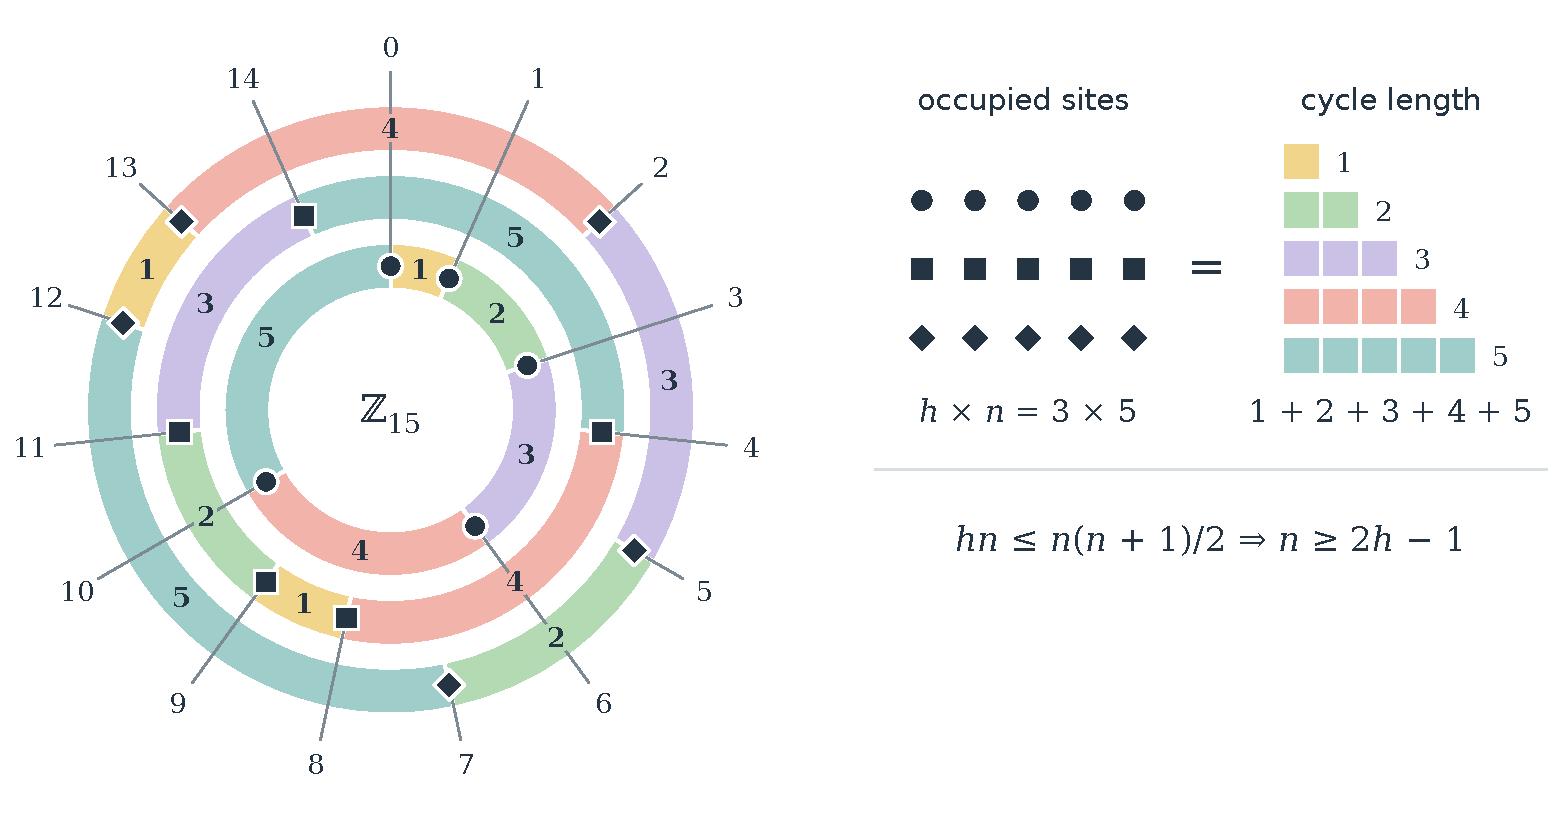
\includegraphics[width=\linewidth]{figures/fig1-optimal-corral.pdf}
\caption{An optimal corral of height \(3\) and order \(5\). Each ring is a row on \(\mathbb Z_{15}\), and its arcs are labelled and coloured by clockwise gap length. Each numbered spoke ends at the row point occupying that site. At right, the \(3\cdot5\) occupied sites fill the cycle of length \(1+2+3+4+5\).}
\label{fig:fig1-optimal-corral}
\end{figure}

Binięda, Dębski, Gutowski and Milewski conjecture existence for every \(n\geq2h-1\), prove it for \(n\geq2h\), and compute optimal examples through height 50 \cite{BDGM26}. Nakamigawa constructed well-dispersed optimal corrals at heights \(a2^b\), where \(a\in\{2,5,6,7\}\) and \(b\) is a nonnegative integer \cite{Nak15}. In a well-dispersed corral the cycle is divided into consecutive blocks of \(h\) sites starting at zero, and each block contains one point of each row.

We prove the optimal-order case \(n=2h-1\) of \cite[Conjecture 1]{BDGM26}.

\statementstart\textbf{Theorem 1 (Optimal existence).} For every positive integer \(h\), there exists a breakfree corral of height \(h\) and order \(2h-1\).

\statementstart\textbf{Corollary 2.} For positive integers \(h,n\), a breakfree corral of height \(h\) and order \(n\) exists if and only if \(n\geq2h-1\).

The necessity is the counting bound. Theorem 1 gives equality and \cite[Theorem 3]{BDGM26} supplies the larger orders. Our even construction uses complementary reflected prefix sets. For odd \(h\geq5\), we partition two shorter cycles into \(h\) rows each, with two points in each row of the second cycle. We pair the rows and join them so that the two new gaps have the same lengths, in some order, as the two removed wrap gaps. The underlying graceful and terrace ideas have classical antecedents in \cite{HOS19} and \cite{OW11}.

\begin{samepage} At optimal order a corral is a partition of the cycle \(\mathbb Z_{h(2h-1)}\) into \(h\) unlabelled rows, each with the cyclic gaps \(1,\ldots,2h-1\) in some order. Two partitions are equivalent if a common rotation or reflection takes one to the other. A partition is \emph{asymmetric} if the identity is the only such isometry taking its collection of rows to itself. Write \(A_h\) for the number of equivalence classes of asymmetric optimal corrals and \(P_h\) for the number of physical partitions before taking the dihedral quotient, including symmetric ones. \par\end{samepage}

The lower bound in Theorem 10 applies at every sufficiently large height. Together with the upper bound in Theorem 8, it gives \[
 \log A_h=\Theta(h^2\log h)\qquad(h\to\infty).
\] For the lower bound, we extend a short prescribed path to a terrace and use independent Latin-square choices to build distinct asymmetric physical partitions.

Theorem 9 constructs rainbow path factors in finite abelian groups of sufficiently large odd order. Subject to its size and sum conditions, we can prescribe the vertex set, the nonzero differences and the sets of starts and ends. The vertex set may omit a fixed positive fraction of the group. The construction determines the endpoint pairing and yields a single cycle when both endpoint sets are empty. Its single-path case supplies the terrace completion used in Theorem 10. Proposition 9.1 gives an upper bound of \(1/4\) on the universal missing-vertex tolerance, already for a single path.

\statementstart\textbf{Theorem 3 (Explicit diversity).} Let \(h=2k\), where \(k\geq3\) is odd. There is an explicit family of optimal corrals meeting exactly \[
 \frac{2^{(k-1)^2}-2^{(k-1)^2/2}}{2}
\] asymmetric physical dihedral orbits. In particular, \(\log_2 A_h\geq h^2/4-h-1\).

The formula counts the asymmetric orbits represented in this family. Its two-row supports admit independent decompositions. A fixed pair of rows restricts the isometries between family members to the identity and one reflection.

\statementstart\textbf{Theorem 7 (Prime-height asymmetry).} Every optimal corral of odd prime height is asymmetric.

\statementstart\textbf{Theorem 8 (A global upper bound).} For \(h\geq2\), set \(n=2h-1\), \(M=hn\), \((n)_j=n(n-1)\cdots(n-j+1)\), and \[
 B_h=\prod_{j=1}^{h-2}\frac{(n-j)^j}{(n)_j}.
\] Then \[
 P_h\leq(n!)^{h-1}B_h,\qquad
 A_h\leq\frac{(n!)^{h-1}B_h}{2M},\qquad
 B_h\leq\exp\!\left(-\frac{(h-2)(h-1)h}{6(2h-1)}\right).
\]

The bound on \(P_h\) applies to the total number of optimal partitions. The proof uses the fact that every interval of \(2h-1\) consecutive sites meets each row. Appendix A gives a further constructed family and an exact count for that family.

The Actual Remainder Lemma in Section B.3.3 gives a quantitative group-matching result. A categorical sample for the endpoint roles and an independent colour sample give one high-probability event for all admissible later targets. The joint budget is a fixed fraction of the group order and covers target edits, a balanced zero-sum reserve and a small preselected matching. The lemma also allows a later edge ban with bounded degree at each tagged vertex. Outside the reserve, the matching contains the preselected edges, avoids the forbidden edges and leaves \(O(\sqrt n\log^{3/2}(en))\) unmatched vertices per role. The remainder has equal role sizes and total signed sum zero. Each of its coordinates is nonzero, and the remainder may be empty. The rate uses the hypergraph matching theorem of Alon, Kim and Spencer \cite{AKS97}.

In the exact-matching step for Theorem 9, we apply the lemma with a reserved absorbing core and empty sets of preselected and forbidden edges. We then match the core and the remainder together.

Sections 2--5 give the existence constructions, with a worked example at height seven in Section 5.1. Sections 6 and 7 study explicit diversity, symmetry and the global upper bound. Section 8 states the group-theoretic endpoint theorem and derives the all-height lower bound using a Latin-square construction. Section 9 describes the software and formal scope, and Section 10 lists further questions. Appendix A gives a separately counted family, and Appendix B contains the endpoint proof.

\hypertarget{cyclic-gaps-and-two-elementary-constructions}{%
\section{Cyclic gaps and two elementary constructions}\label{cyclic-gaps-and-two-elementary-constructions}}

For a positive integer \(m\), write \([m]=\{1,\ldots,m\}\); for integers \(a,b\), write \([a,b]=\{x\in\mathbb Z:a\leq x\leq b\}\), which is empty when \(a>b\). For a positive integer \(M\), identify \(\mathbb Z_M\) with \(\{0,\ldots,M-1\}\). For positive integers \(h,n\), a breakfree corral of height \(h\) and order \(n\) is a collection of permutations \(\rho_i\) of \([n]\) and integer shifts \(\tau_i\), \(0\leq i<h\), such that the \(hn\) residues \[
 \left(\tau_i+\sum_{k=1}^{j}\rho_i(k)\right)\bmod w,
 \qquad 0\leq i<h,\quad 1\leq j\leq n,\qquad
 w=\frac{n(n+1)}2,
\] are pairwise distinct. Thus \(hn\leq w\), giving \(n\geq2h-1\).

For a nonempty set \(R=\{x_0<\cdots<x_{r-1}\}\subseteq\mathbb Z_M\), its positive cyclic gaps are

\[
 x_1-x_0,\ldots,x_{r-1}-x_{r-2},x_0+M-x_{r-1}.
\]

For a singleton the gap is \(M\). At \(n=2h-1\), it suffices to partition \(\mathbb Z_{h(2h-1)}\) into \(h\) sets whose gap multiset is \([2h-1]\). Indeed, the gaps in cyclic order form the required permutation, and the least point can be used as its shift. The partial sums visit the next point and finally return to the least point. Conversely, a positive permutation summing to \(w\) makes one complete winding around the cycle, so its partial sum set has precisely that cyclic gap multiset.

\statementstart\textbf{Lemma 4.} Let \(h,p\) be positive integers, let \(M=hp\), and let \(P\subseteq\mathbb Z_M\) project bijectively onto \(\mathbb Z_p\). Then the sets \(P+ps\), \(0\leq s<h\), partition \(\mathbb Z_M\).

\labelledparagraphstart\textbf{Proof.} Above each residue modulo \(p\), there is one point of \(P\). Its \(h\) translates by \(ps\) are exactly the \(h\) points of that fiber. Different fibers are disjoint. \(\square\)

We also use a concatenation identity. Let \(U,V\) be positive integers, and let \(C\subseteq\{0,\ldots,U-1\}\) and \(D\subseteq\{0,\ldots,V-1\}\) be nonempty sets. Set

\[
 f_C=\min C,\quad t_C=U-\max C,\qquad
 f_D=\min D,\quad t_D=V-\max D.
\]

Their local wrap gaps are \(f_C+t_C\) and \(f_D+t_D\). In \(C\cup(U+D)\subseteq\mathbb Z_{U+V}\), these two gaps are replaced by

\begin{equation}
t_C+f_D,\qquad t_D+f_C.
\tag{1}\label{eq:1}
\end{equation}

\statementstart\textbf{Lemma 5.} If \(f_C=f_D\) or \(t_C=t_D\), the cyclic gap multiset of \(C\cup(U+D)\) is the union of the cyclic gap multisets of \(C\) and \(D\).

\labelledparagraphstart\textbf{Proof.} All interior gaps are unchanged. Under either stated equality, the two gaps in (1) are the two old wrap gaps, possibly exchanged. \(\square\)

\hypertarget{even-heights}{%
\section{Even heights}\label{even-heights}}

Let \(h=2k\), \(n=4k-1\), \(p=2n\), and \(w=kp\). List \(1,\ldots,h-1\) as \[
 (a_0,\ldots,a_{h-2})=(h-1,h-3,\ldots,1,\ h-2,h-4,\ldots,2),
\] and form the positive word

\begin{equation}
G=(a_0,2h-a_0,\ldots,a_{h-2},2h-a_{h-2},h).
\tag{2}\label{eq:2}
\end{equation}

Its entries are exactly \([n]\), and their sum is \(w\). Put

\begin{equation}
c=\begin{cases}
 k-1,&k\text{ even},\\
 5k-2,&k\text{ odd}.
 \end{cases}
\tag{3}\label{eq:3}
\end{equation}

For each \(0\leq j<k\), take one row with gap word \(G\) and shift \(jp\), and one with the reversal of \(G\) as gap word and shift \(c+jp\). We show that the rows partition the physical cycle.

Let \(R\) be the proper prefix set of \(G\) in \(\mathbb Z_w\), including zero. To check disjointness of the translates, let \(A\) be the image of \(R\) in \(\mathbb Z_p\). Each two-entry pair in (2) sums to \(2h=n+1\). The prefix sums at the pair boundaries are \(E_j=2hj\), \(0\leq j<h\). They are even and have residue \(j\) modulo \(n\). Reduction modulo \(n\) is a bijection from either parity class in \(\mathbb Z_p\) to \(\mathbb Z_n\).

For an even label \(a_j=2r\), \(1\leq r<k\), the order gives \(j=h-1-r\), so its even middle point has residue \(h-1+r\) modulo \(n\). For an odd label \(a_j=2r+1\), \(0\leq r<k\), its slot is \(j=k-1-r\), so its odd middle point has residue \(k+r\). Hence the residues of the even and odd quotient points of \(A\), respectively, are the intervals

\[
 X=[0,3k-2],\qquad Y=[k,2k-1].
\]

There are \((3k-1)+k=n\) distinct quotient points in the two parity classes, so the projection of \(R\) is injective. The integer \(c\) is odd and \(c\equiv k-1\pmod n\). Reflection \(x\mapsto c-x\) exchanges the parity classes and sends \(Y\) to \([3k-1,4k-2]=\mathbb Z_n\setminus X\). By involution it also sends \(X\) to the complement of \(Y\). Thus \(A\) and \(c-A\) partition \(\mathbb Z_p\), including when \(k=1\).

The \(k\) translates \(R+jp\) fill the physical fibers above \(A\), and the translates \(c-R+jp\) fill those above \(c-A\). Reversing \(G\) reflects its prefix set because its total sum is \(w\). The rows therefore partition \(\mathbb Z_w\), with every cyclic gap in \([n]\) occurring once, including the wrap. This proves Theorem 1 for every even height. \autoref{fig:fig2-even-grid} shows the residue classes and the translates at height six.

\begin{figure}[!htbp]
\centering
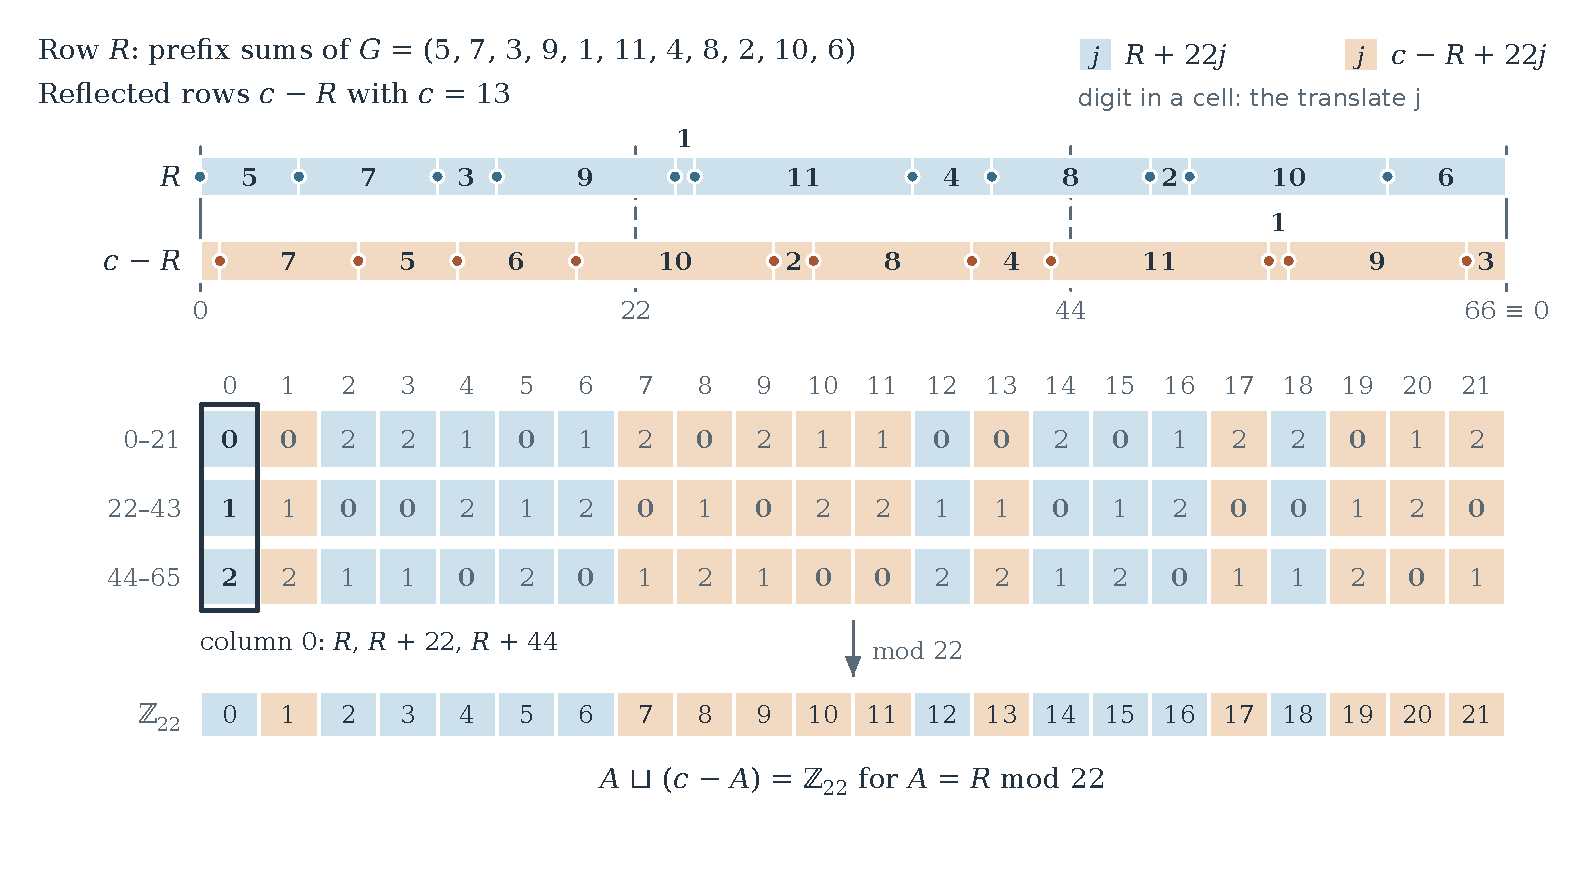
\includegraphics[width=\linewidth]{figures/fig2-even-grid.pdf}
\caption{The even construction at height six on the \(66\)-site cycle. The upper strips show \(R\) and its reflection \(c-R\) for \(c=13\). In the grid, a column is a residue modulo \(22\), and the digit \(j\) denotes the translate by \(22j\). The outlined column contains one point of each translate of \(R\). The reduction below shows the complementary images of the two rows.}
\label{fig:fig2-even-grid}
\end{figure}

\hypertarget{odd-heights-at-least-five}{%
\section{Odd heights at least five}\label{odd-heights-at-least-five}}

Write \(h=2A+3\), \(A\geq1\), and set \[
 K=4A+3=2h-3,\qquad U=hK,\qquad W=U+2h=h(2h-1).
\] We partition \(\mathbb Z_U\) and \(\mathbb Z_{2h}\) separately into \(h\) rows each. Each two-point row on the smaller cycle supplies the two gaps missing from a row on the larger cycle.

\hypertarget{a-positive-word-and-the-first-factor}{%
\subsection{A positive word and the first factor}\label{a-positive-word-and-the-first-factor}}

Concatenate the following pieces, in order, to form \(G\): \begin{equation}
\begin{gathered}
 (K+2,K-1),\\
 (K-3-4j,\,4j+5)\quad(0\leq j<A),\\
 (K+1),\\
 (4j+2,\,K-4-4j)\quad(0\leq j<A-1),\\
 (K-5,1).
\end{gathered}
\tag{4}\label{eq:4}
\end{equation} Empty ranges contribute no entries. The even entries are precisely the positive even integers through \(K+1\). The odd entries are precisely the positive odd integers through \(K+2\), except \(3\) and \(K\). Thus \(G\) has \(K\) entries, gap multiset \([2h-1]\setminus\{3,K\}\), and sum \[
 \frac{(2h-1)2h}{2}-(3+K)=hK=U.
\]

Let \(P\) be its proper prefix set, beginning at zero. Its members are \begin{equation}
\begin{array}{ll}
 0,\ K+2, &\\
 L_j=(j+2)K+2j+1 &(0\leq j\leq A),\\
 H_j=(j+3)K-2j-2 &(0\leq j<A),\\
 E_j=(A+3+j)K+2A+2-2j &(0\leq j<A),\\
 F_j=(A+3+j)K+2A+4+2j &(0\leq j<A-1),\\
 U-1.&
\end{array}
\tag{5}\label{eq:5}
\end{equation} They occur in the order \[
 (0,K+2),\ (L_j,H_j)_{j=0}^{A-1},\ L_A,
 (E_j,F_j)_{j=0}^{A-2},\ E_{A-1},\ U-1,
\] with each indexed pair expanded in increasing order and empty ranges omitted. The first indexed pairs in (4) sum to \(K+2\) and the second to \(K-2\), yielding (5). Modulo \(K\), the prefixes have residues \(0,2,K-1\), the odd ranges \(1,3,\ldots,2A+1\) and \(2A+3,2A+5,\ldots,4A+1\), and the even ranges \(4,6,\ldots,2A+2\) and \(2A+4,2A+6,\ldots,4A\). These are all residues exactly once, including when \(A=1\).

Set \(z=2A\). By Lemma 4, the \(h\) rows \begin{equation}
C_s=\{(p+z+Ks)\bmod U:p\in P\},\qquad 0\leq s<h,
\tag{6}\label{eq:6}
\end{equation} partition \(\mathbb Z_U\). Each has the cyclic gap multiset of \(G\).

\hypertarget{the-two-point-factor-and-the-cut-certificate}{%
\subsection{The two-point factor and the cut certificate}\label{the-two-point-factor-and-the-cut-certificate}}

On \(\mathbb Z_{2h}\), define \begin{equation}
D_t=\{2t,(2t+3)\bmod 2h\},\qquad 0\leq t<h.
\tag{7}\label{eq:7}
\end{equation} The points \(2t\) fill the even residues and the points \((2t+3)\bmod 2h\) fill the odd residues. The rows therefore partition \(\mathbb Z_{2h}\). Each has gaps \(3\) and \(2h-3=K\). Write \(f_D(t)=\min D_t\) for the first point measured from the cut at zero and \(t_D(t)=2h-\max D_t\) for the tail deficit. Then \begin{equation}
(f_D(t),t_D(t))=
 \begin{cases}
 (2t,K-2t),&0\leq t\leq h-2,\\
 (1,2),&t=h-1.
 \end{cases}
\tag{8}\label{eq:8}
\end{equation}

To compute the first point and tail deficit of a translated core row, look at the gap crossing the cut at \(U\). Suppose a proper prefix \(p\), followed by a gap \(g\), satisfies \(p+q=U-\delta\), where \(0<\delta\leq g\) and \(0\leq q<U\). Include the final prefix sum \(U\) as the next copy of zero before translating. In the translated list, \(p+q\) is the last point below the cut and \(p+q+g\) is the first at or above it. After reduction modulo \(U\), the first point is \(f_C=g-\delta\) and the tail deficit is \(t_C=\delta\). Equality \(\delta=g\) places a point right at the cut.

For \(q=z+Ks\), the needed cut certificates are:

\begin{longtable}[]{@{}
  >{\raggedright\arraybackslash}p{(\columnwidth - 6\tabcolsep) * \real{0.2500}}
  >{\raggedright\arraybackslash}p{(\columnwidth - 6\tabcolsep) * \real{0.2500}}
  >{\raggedright\arraybackslash}p{(\columnwidth - 6\tabcolsep) * \real{0.2500}}
  >{\raggedright\arraybackslash}p{(\columnwidth - 6\tabcolsep) * \real{0.2500}}@{}}
\toprule\noalign{}
\begin{minipage}[b]{\linewidth}\raggedright
Owner \(s\)
\end{minipage} & \begin{minipage}[b]{\linewidth}\raggedright
Prefix \(p\) before the cut
\end{minipage} & \begin{minipage}[b]{\linewidth}\raggedright
Following gap \(g\)
\end{minipage} & \begin{minipage}[b]{\linewidth}\raggedright
\(\delta=U-p-z-Ks\)
\end{minipage} \\
\midrule\noalign{}
\endhead
\bottomrule\noalign{}
\endlastfoot
\(0\leq s<A\) & \(E_{A-1-s}\) & \(4A-2-4s\) & \(2A-1-2s\) \\
\(s=A\) & \(L_A\) & \(K+1\) & \(2\) \\
\(A<s\leq2A\) & \(L_{2A-s}\) & \(4(s-A)\) & \(2s-2A+2\) \\
\(s=2A+1\) & \(K+2\) & \(K-1\) & \(2A+1\) \\
\(s=2A+2\) & \(0\) & \(K+2\) & \(2A+3\) \\
\end{longtable}

Indeed, the first three translated prefixes are respectively \begin{equation}
\begin{aligned}
 E_{A-1-s}+z+Ks&=(h-1)K+2A+4+2s,\\
 L_A+z+KA&=(h-1)K+4A+1,\\
 L_{2A-s}+z+Ks&=(h-1)K+6A-2s+1.
\end{aligned}
\tag{9}\label{eq:9}
\end{equation} The last two are \((h-1)K+2A+2\) and \((h-1)K+2A\). Subtracting each from \(U=hK\) gives the table's deficits. The listed gaps follow from (4), including the final \(E\)-gap \(K-5\). The first and fourth cases have \(g=2\delta\); in the third, \(g-\delta=2(s-A-1)\geq0\), and in the second and fifth it is \(K-1\) and \(2A+2\), respectively. Hence every table entry satisfies \(0<\delta\leq g\), even at \(A=1\).

\hypertarget{matching-the-seams-and-the-physical-inverse}{%
\subsection{Matching the seams and the physical inverse}\label{matching-the-seams-and-the-physical-inverse}}

Pair \(C_s\) with a two-point row so that their first points or their tail deficits agree, as required by Lemma 5. Start with the assignment \(\rho(s)=(s+A+2)\bmod h\) and exchange the partners assigned to core rows \(h-2,h-1\), obtaining the permutation \(\pi\). Equation (8) and the cut table give the required equalities:

\begin{itemize}
\tightlist
\item
  If \(0\leq s<A\), then \(\pi(s)=s+A+2\) and \(t_D=K-2\pi(s)=2A-1-2s=t_C\).
\item
  If \(s=A\), then \(\pi(s)=h-1\) and \(t_D=t_C=2\).
\item
  If \(A<s\leq2A\), then \(\pi(s)=s-A-1\) and \(f_D=2s-2A-2=g-\delta=f_C\).
\item
  For \(s=h-2,h-1\), the swapped images are \(A+1,A\); their respective tail deficits are \(2A+1,2A+3\), as required.
\end{itemize}

Set \begin{equation}
R_s=C_s\cup\{U+y:y\in D_{\pi(s)}\}.
\tag{12}\label{eq:12}
\end{equation} The two local partitions and bijectivity of \(\pi\) give a partition of \(\mathbb Z_W\) into \(h\) rows with \(2h-1\) sites each. Lemma 5 preserves the two removed wrap gaps. Every \(R_s\) therefore has cyclic gap multiset \[
 \bigl([2h-1]\setminus\{3,K\}\bigr)\cup\{3,K\}=[2h-1].
\]

This construction also has a direct site-to-row inverse. If \(x<U\), choose the unique \(p\in P\) with \(p\equiv x-z\pmod K\) and return \begin{equation}
s=\frac{(x-z-p)\bmod U}{K}.
\tag{13}\label{eq:13}
\end{equation} If \(x\geq U\), put \(y=x-U\). Its two-point owner is \(t=y/2\) when \(y\) is even and \(t=((y-3)/2)\bmod h\) when \(y\) is odd; the full owner is \(\pi^{-1}(t)\).

\hypertarget{small-odd-heights}{%
\section{Small odd heights}\label{small-odd-heights}}

At \(h=1\), the singleton \(\{0\}\subseteq\mathbb Z_1\) has gap one. At \(h=3\), the rows \[
 \{0,1,3,6,10\},\quad\{4,8,9,11,14\},\quad\{2,5,7,12,13\}
\] partition \(\mathbb Z_{15}\), with gap words \((1,2,3,4,5)\), \((4,1,2,3,5)\) and \((3,2,5,1,4)\). Together with Sections 3--4, these cases prove Theorem 1 at every positive height. \(\square\)

\hypertarget{an-example-at-height-seven}{%
\subsection{An example at height seven}\label{an-example-at-height-seven}}

Take \(A=2\), \(K=11\), \(U=77\), \(W=91\), and \(z=4\). The core word is \[
 G=(13,10,8,5,4,9,12,2,7,6,1),
\] and the assignment is \(\pi=(4,5,6,0,1,3,2)\). The first core row is \[
 C_0=\{3,4,17,27,35,40,44,53,65,67,74\},
\] and its partner is \(D_4=\{8,11\}\). Both have tail deficit three. Their local wrap gaps are six and eleven; the new seams are \(3+8=11\) and \(3+3=6\). The completed row is \[
 R_0=\{3,4,17,27,35,40,44,53,65,67,74,85,88\}.
\] Its cyclic gaps are \((1,13,10,8,5,4,9,12,2,7,11,3,6)\), exactly \([13]\). The accompanying \href{supplement/examples/height-seven.json}{height-seven certificate} lists all seven rows. \autoref{fig:fig3-odd-construction} compares their two seams with the original wrap gaps.

\begin{figure}[!htbp]
\centering
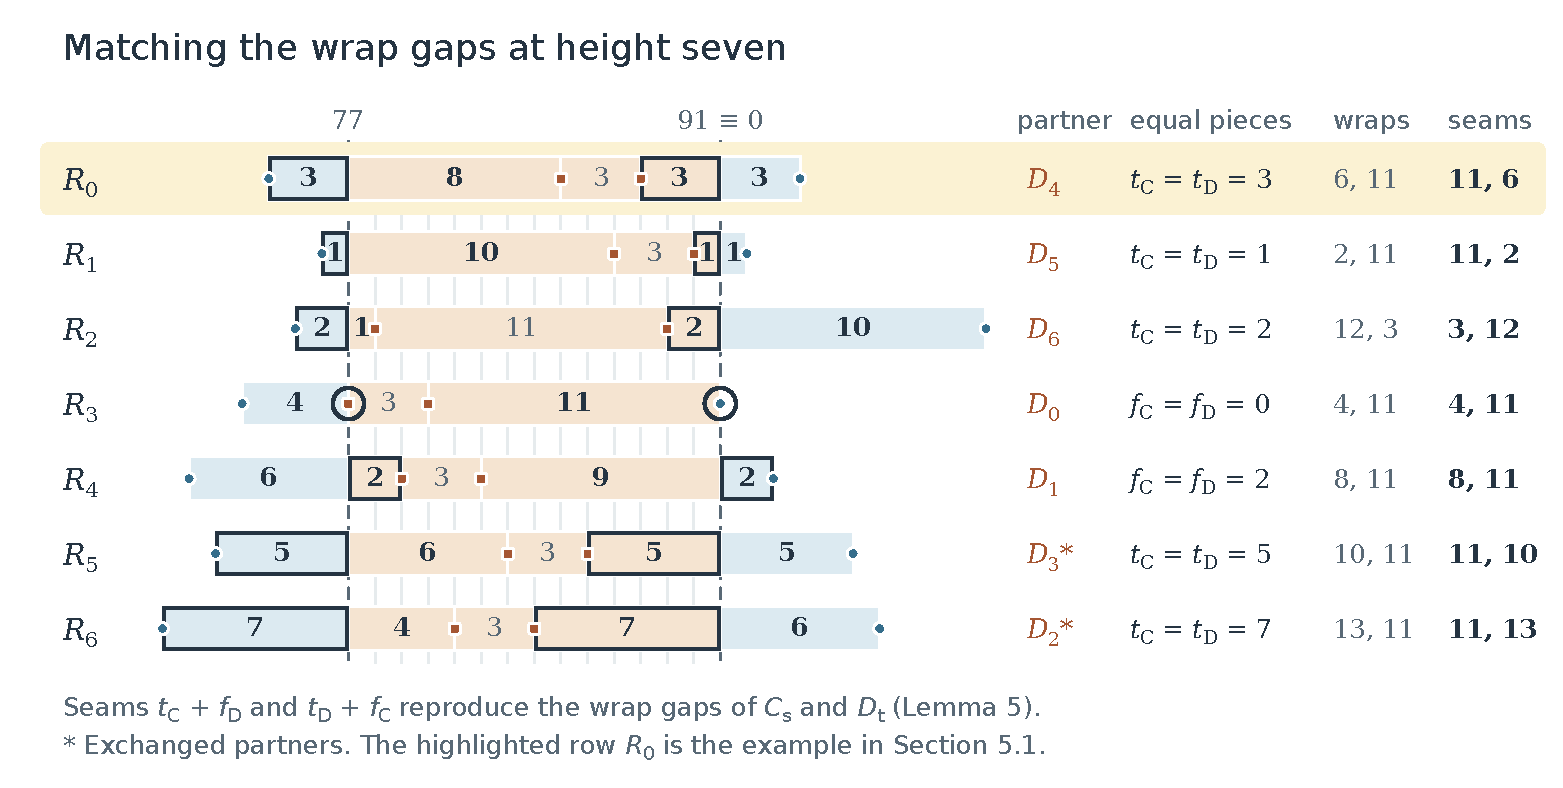
\includegraphics[width=\linewidth]{figures/fig3-odd-construction.pdf}
\caption{The seams of the seven rows at the cuts \(77\) and \(91\equiv0\). The outlines mark two equal distances from the cuts, measured either forward to the first points or backward to the last points. The last two columns compare the original wrap lengths with the new seam lengths. The highlighted row is \(R_0\). Asterisks mark the two partners exchanged relative to the cyclic assignment.}
\label{fig:fig3-odd-construction}
\end{figure}

\hypertarget{an-explicit-family-with-quadratic-diversity}{%
\section{An explicit family with quadratic diversity}\label{an-explicit-family-with-quadratic-diversity}}

We prove Theorem 3. Write \[
 h=4m+2=2k,\quad k=2m+1,\quad m\geq1,\qquad
 n=2h-1,\quad M=hn,\quad p=2n.
\] Let \(R\) be the row beginning at zero in the even-height construction of Section 3. Its proper prefix set is \begin{equation}
\begin{split}
 R={}&\{2hj:0\leq j\leq h-1\}\\
 &\cup\{(2j+1)(h-1):0\leq j\leq k-1\}\\
 &\cup\{2(j+1)(h-1):k\leq j\leq h-2\}. 
\end{split}
\tag{D1}\label{eq:D1}
\end{equation} Put \(C=h^2-1\), \(g(x)=C-x\), \(U=R\cup g(R)\), and \(U_j=U+jp\) for \(j\in\mathbb Z_k\). Since the reflection parameter in Section 3 is \(c=5k-2\) for odd \(k\), \begin{equation}
C-c=(k-1)n=\frac{k-1}{2}p.
\tag{D2}\label{eq:D2}
\end{equation} Thus \(R+jp\) and \(g(R)+jp\) are two of the rows already constructed in Section 3. The supports \(U_j\) are disjoint and partition \(\mathbb Z_M\). We first construct multiple decompositions of a single support into two rows. Paired switches preserve the cyclic gap multiset of each row. In the full family we retain the original pair on one support to control which physical isometries can identify two partitions.

\hypertarget{a-family-of-decompositions-of-one-support}{%
\subsection{A family of decompositions of one support}\label{a-family-of-decompositions-of-one-support}}

Choose binary strings \(\eta,\varepsilon\), indexed by \(0,\ldots,k-1\), such that \begin{equation}
\begin{gathered}
 \eta_j=\eta_{k-1-j},\qquad \eta_0=\eta_{k-1}=1,\\
 \varepsilon_j=\varepsilon_{k-1-j},\qquad
 \varepsilon_0=\varepsilon_{k-1}=1,\qquad
 \varepsilon_1=\varepsilon_{k-2}=0. 
\end{gathered}
\tag{D3}\label{eq:D3}
\end{equation} For \(k=3\) the last two indices are the same. These conditions leave \(m\) free bits in \(\eta\) and \(m-1\) in \(\varepsilon\). Define \begin{equation}
\begin{split}
 A(\eta,\varepsilon)={}&\{0\}\\
 &\cup\{(2j+1+\eta_j)(h-1):0\leq j<k\}\\
 &\cup\{2hi-(i\bmod2):1\leq i<k\}\\
 &\cup\{(h+2+2j)(h-1)+\varepsilon_j:0\leq j<k\}\\
 &\cup\{2h(k+1+2r),\;2h(k+1+2r)+h-1:0\leq r<m\}, 
\end{split}
\tag{D4}\label{eq:D4}
\end{equation} and let \(B(\eta,\varepsilon)=U\setminus A(\eta,\varepsilon)\). The displayed points are their ordinary representatives in \([0,M-1]\).

\statementstart\textbf{Lemma 6.} Every choice in (D3) gives two valid rows \(A,B\) partitioning \(U\). The choices give \(2^{k-2}\) different unordered decompositions.

\labelledparagraphstart\textbf{Proof.} Write \begin{equation}
\begin{array}{lll}
 t_j=(2j+1+\eta_j)(h-1),&&s_j=(2j+2-\eta_j)(h-1),\\
 d_i=2hi-(i\bmod2),&&e_i=2hi-(1-(i\bmod2)),\\
 u_j=(h+2+2j)(h-1)+\varepsilon_j,&&
 z_j=(h+2+2j)(h-1)+1-\varepsilon_j.
\end{array}
\tag{D5}\label{eq:D5}
\end{equation} Substitution in (D1) and its reflection gives the following disjoint decomposition of \(U\): the points \(0,C\); the pairs \(t_j,s_j\), \(d_i,e_i\), and \(u_j,z_j\) in their displayed index ranges; and the fixed points \[
\begin{array}{ll}
 v_r=2h(k+1+2r),\quad w_r=v_r+h-1 &(0\leq r<m),\\
 h^2,\ M-1,\quad v'_r=2h(k+2+2r),\quad w'_r=v'_r+h-1
 &(0\leq r<m-1).
\end{array}
\] The point \(0\) belongs to \(A\) and \(C\) belongs to \(B\). The first member of each pair and the \(v_r,w_r\) belong to \(A\). The second member and the remaining fixed points belong to \(B\). There are \(2n\) distinct points in the displayed decomposition, and each row has \(n\) points.

The increasing order in \(A\) begins \[
 0,t_0,d_1,t_1,d_2,t_2,\ldots,d_{k-1},t_{k-1},u_0
\] and then runs through \begin{equation}
u_{2r},v_r,u_{2r+1},w_r,u_{2r+2}\qquad(0\leq r<m),
\tag{D6}\label{eq:D6}
\end{equation} with consecutive blocks sharing their indicated endpoints. It wraps from \(u_{k-1}\) to zero. The order in \(B\) begins \[
 s_0,e_1,s_1,\ldots,e_{k-1},s_{k-1},C,h^2,z_0,z_1,
\] continues through \begin{equation}
z_{2r+1},v'_r,z_{2r+2},w'_r,z_{2r+3}\qquad(0\leq r<m-1),
\tag{D7}\label{eq:D7}
\end{equation} and finishes with \(z_{k-1},M-1\), wrapping to \(s_0\). Empty ranges are omitted. The inequalities follow directly from (D5); in particular each moving point stays strictly between the same fixed neighbours for both of its choices.

\hypertarget{the-baseline-palettes}{%
\subsection{The baseline palettes}\label{the-baseline-palettes}}

Set all free bits in (D3) to zero and put \(\delta_i=i\bmod2\). The cyclic order of \(A\) in Section 6.1 gives the following gap word, starting at zero:

\begin{enumerate}
\def\labelenumi{\arabic{enumi}.}
\tightlist
\item
  Start with \(2h-2\).
\item
  For \(1\leq i\leq2m\), append \((a_i,b_i)\), where \(a_1=1\), \(a_i=h-1+2i-\delta_i\) for \(i\geq2\), \(b_i=h-1-2i+\delta_i\) for \(i<2m\), and \(b_{2m}=h\).
\item
  Append \(n\).
\item
  For \(0\leq r<m\), append \((h+2+4r-[r=0],h-4-4r,4r+3,2h-5-4r+[r=m-1])\).
\item
  Append the wrap \(h-1\).
\end{enumerate}

The cyclic order of \(B\) in Section 6.1 gives the following gap word, starting at \(C\):

\begin{enumerate}
\def\labelenumi{\arabic{enumi}.}
\tightlist
\item
  Start with \((1,h-2,n)\).
\item
  For \(0\leq r<m-1\), append \((h+3+4r,h-5-4r,4r+4,2h-6-4r)\).
\item
  Append \((2h-3,h-1,h)\).
\item
  For \(1\leq i\leq2m\), append \((a'_i,b'_i)\), where \(a'_1=h+1\), \(a'_i=2i-1+\delta_i\) for \(i\geq2\), \(b'_i=2h-1-2i-\delta_i\) for \(i<2m\), and \(b'_{2m}=2\).
\item
  Append \(2h-2\), closing at \(C\).
\end{enumerate}

All entries are positive. Substituting \(h=4m+2\) and collecting residues modulo four in \textbf{either} word gives the following disjoint progressions: \[
\begin{array}{c|l}
 0&4,8,\ldots,8m\\
 1&1,5,\ldots,8m+1\\
 2&2,6,\ldots,8m+2\\
 3&3,7,\ldots,8m+3.
\end{array}
\] For example, the zero-residue entries of the \(A\) word are supplied by the odd-indexed \(b_i\), the last entry of the final upper block, and the first entries of the upper blocks with \(r\geq1\); they form respectively \(4,\ldots,4m\), \(4m+4\), and \(4m+8,\ldots,8m\). In the \(B\) word they come from the third entries of its upper blocks, the initial gap \(h-2\), and the odd-indexed \(b'_i\). The other residue classes follow by the displayed formulas. Empty ranges at \(m=1\) contribute nothing. Consequently both baseline rows have the complete palette \([n]\), including their physical wrap gaps.

\hypertarget{simultaneous-switches}{%
\subsection{Simultaneous switches}\label{simultaneous-switches}}

\autoref{fig:fig4-switch} shows a switch on \(U_1\) at height six.

\begin{figure}[H]
\centering
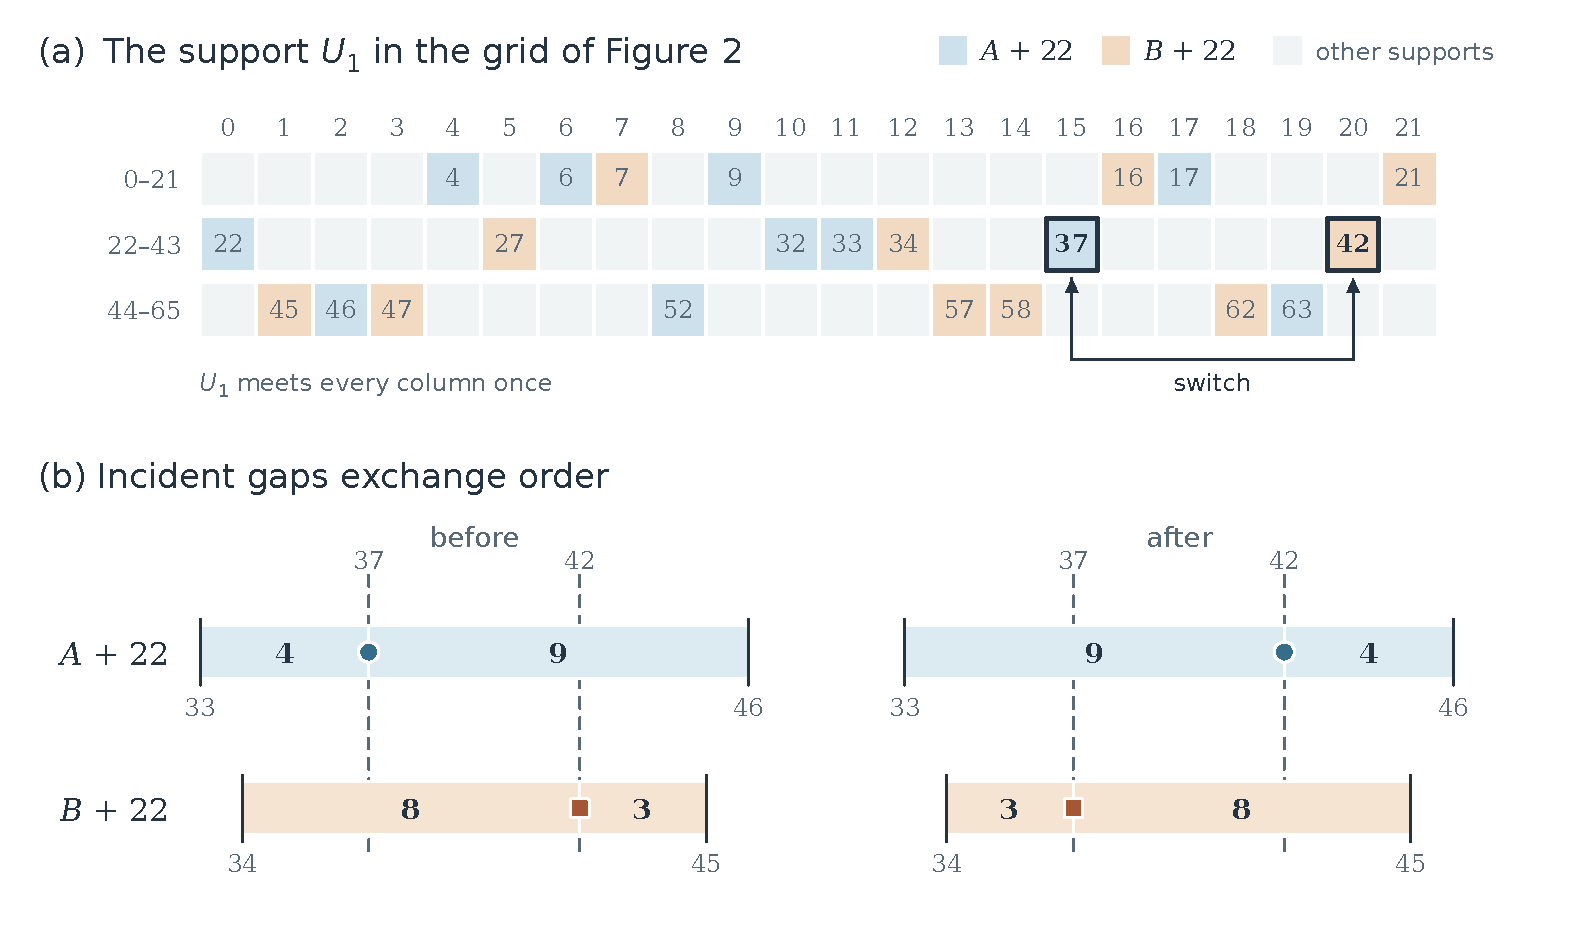
\includegraphics[width=\linewidth]{figures/fig4-switch.pdf}
\caption{A switch on the support \(U_1\) at height six. The upper grid shows \(U_1\) in the residue classes of \autoref{fig:fig2-even-grid} and marks sites \(37\) and \(42\). Below, these sites exchange owners in \(A+22\) and \(B+22\). Each row retains its two incident gap lengths in the opposite order. At height six the moving index is its own partner.}
\label{fig:fig4-switch}
\end{figure}

For an interior index \(j\), write \(\delta_j=j\bmod2\). When \(\eta_j=0\), the two gaps incident to \(t_j\) in \(A\) are \begin{equation}
(h-1-2j+\delta_j,\ h+2j+\delta_j).
\tag{D8}\label{eq:D8}
\end{equation} Changing \(\eta_j\) to one adds \(h-1\) to the first and subtracts \(h-1\) from the second. The paired index \(k-1-j\) has the same parity, and its old pair is the new pair at \(j\) in reverse order. At the complementary point \(s_j\) of \(B\), the old pair is \begin{equation}
(2h-1-2j-\delta_j,\ 2j+2-\delta_j),
\tag{D9}\label{eq:D9}
\end{equation} and the point moves in the opposite direction. Its paired-index calculation again preserves the combined multiset. If the index is its own partner, the two incident values simply exchange.

For a free upper index \(2\leq j\leq k-3\), the old incident pair at \(u_j\), when \(\varepsilon_j=0\), is \begin{equation}
\begin{cases}
 (2h-1-2j,h+2+2j),&j\text{ even},\\
 (h-2-2j,2j+1),&j\text{ odd}.
 \end{cases}
\tag{D10}\label{eq:D10}
\end{equation} Raising \(\varepsilon_j\) adds one to the incoming gap and subtracts one from the outgoing gap. If the old pair at \(j\) is \((a,b)\), the old pair at \(k-1-j\) is \((b-1,a+1)\), proving preservation. At the complementary point \(z_j\) the old pair is \begin{equation}
\begin{cases}
 (h-1-2j,2j),&j\text{ even},\\
 (2h-2j,h+1+2j),&j\text{ odd},
 \end{cases}
\tag{D11}\label{eq:D11}
\end{equation} and the opposite unit move has the same paired preservation property.

The moving centres stay between fixed neighbours, and distinct centres have distinct incident edges. Shared fixed neighbours cause no conflict. All lower and upper bit changes may therefore be made simultaneously; the actual cyclic order and the wrap endpoints remain unchanged. The row containing zero is \(A\), and its choices among the pairs in (D5) recover all bits. This proves Lemma 6. \(\square\)

Reflect each decomposition in Lemma 6 by \(g\). The two resulting alphabets are disjoint: the original row \(A\) containing zero contains \(n=2h-1\), while the reflected zero-containing row \(g(B)\) does not, because \(g(n)=2h(k-1)=d_{k-1}\in A\). Their union is a reflection-closed alphabet of \begin{equation}
q=2^{k-1}
\tag{D12}\label{eq:D12}
\end{equation} distinct unordered decompositions. Reflection interchanges its two halves. The original pair \(\{R,g(R)\}\) is outside the alphabet: its row containing zero contains \(h-1\), whereas the zero-containing row of every new pair omits \(h-1\) and contains \(2h-2\).

\hypertarget{the-physical-quotient}{%
\subsection{The physical quotient}\label{the-physical-quotient}}

For a valid row, the unordered pair of gaps immediately adjacent to its unique gap of length \(n\) is invariant under every rotation and reflection. For \(R\) this pair is \(\{1,h-2\}\). For the new rows it is either \(\{h,h+1\}\) or \(\{h-2,h+3\}\); the fixed endpoint values in (D3) give these pairs also at \(m=1\). Thus no new row is physically isometric to \(R\).

A valid row has trivial physical stabilizer. A preserving rotation would cyclically shift its gap word, whose entries are all distinct. A preserving reflection would reverse the odd-length gap cycle and exchange two gap positions, again forcing equal gaps.

Keep \(\{R,g(R)\}\) on \(U_0\), and choose independently one of the \(q\) new decompositions on each remaining \(U_j\). We obtain \[
 N=q^{k-1}=2^{(k-1)^2}
\] distinct physical partitions: the disjoint supports identify every local choice even though the rows are unlabelled. If an isometry carries one family member to another, it must send \(R\) to \(R\) or \(g(R)\), the only target rows with its gap-neighbour invariant. Row rigidity leaves only the identity or \(g\), respectively.

The family is closed under \(g\), and \(g(U_j)=U_{-j}\). Since \(k\) is odd, the \(k-1\) nonzero indices form \((k-1)/2\) pairs. A \(g\)-fixed partition is determined by one arbitrary alphabet letter in each pair, giving precisely \[
 F=q^{(k-1)/2}=2^{(k-1)^2/2}
\] fixed partitions. Every other family member is asymmetric, and its full dihedral orbit meets the family in precisely two members. Hence the number of asymmetric orbits met is \((N-F)/2\), as claimed in Theorem 3. For instance, this gives six such orbits at \(h=6\) and 32,640 at \(h=10\). \(\square\)

\hypertarget{global-symmetry-and-an-upper-bound}{%
\section{Global symmetry and an upper bound}\label{global-symmetry-and-an-upper-bound}}

We first prove Theorem 7. As observed in Section 6, a single valid row has trivial stabilizer under the physical dihedral group: its cyclic gaps are distinct, so no nontrivial rotation or reflection can preserve it. Hence a stabilizer of a corral acts freely on its \(h\) rows, and its order divides \(h\).

If \(h\) is an odd prime, a nontrivial stabilizer would have order \(h\) and contain no reflection. It would therefore be the unique rotation subgroup of order \(h\), generated by translation by \(M/h=n=2h-1\). But every row contains a pair of points at clockwise gap \(n\), so it meets its translate by \(n\). The translated row is distinct by row rigidity, contradicting disjointness of the partition. Thus the stabilizer is trivial. \(\square\)

For Theorem 8, let \(n=2h-1\) and \(M=hn\). A physical row is obtained by choosing a starting site in \(\mathbb Z_M\) and an ordering of the gaps \([n]\). Each physical row has exactly \(n\) such representations, one per starting site on that row. Therefore there are exactly \(h\,n!\) physical rows, and a uniform starting site followed by a uniform gap permutation samples them uniformly.

Every interval of \(n\) consecutive sites meets every row: otherwise the consecutive row points surrounding that interval would have a gap at least \(n+1\). If \(F\) is the union of \(j\) disjoint rows, each such interval therefore meets \(F\) in at least \(j\) sites.

Sample a uniform row \(R\) as above. Its starting point avoids \(F\) with probability \(1-j/h\). Suppose that \(t<j\) gap labels have been exposed, with all visited sites outside \(F\). Condition on the exact exposed history. At least \(j\) of the \(n\) possible next gap lengths land in \(F\), and at most \(t\) of those labels have already been used. The next label is uniform among the \(n-t\) unused labels, so the conditional probability of avoiding \(F\) is at most \[
 \frac{n-j}{n-t}.
\] This bound holds after every surviving history. Consequently \begin{equation}
\Pr(R\cap F=\varnothing)
 \leq\left(1-\frac jh\right)
       \frac{(n-j)^j}{(n)_j}.
\tag{G1}\label{eq:G1}
\end{equation} No independence of the successive avoidance events is used.

Expose an ordered list of \(h-1\) disjoint rows. At the first step there are \(h\,n!\) choices; after \(j\) rows, (G1) gives at most \((h-j)n! (n-j)^j/(n)_j\) choices for the next. Thus the number of ordered prefixes is at most \[
 h!(n!)^{h-1}B_h.
\] The last \(n\) sites determine at most one additional row, while every complete unlabelled partition yields exactly \(h!\) ordered prefixes: choose the omitted row and order the other \(h-1\). Hence \(P_h\leq(n!)^{h-1}B_h\). Every asymmetric physical orbit has exactly \(2M\) physical partitions, giving the asserted bound for \(A_h\).

Finally, using \(\log(1-x)\leq-x\), \[
 \log\frac{(n-j)^j}{(n)_j}
 =\sum_{t=0}^{j-1}\log\!\left(1-\frac{j-t}{n-t}\right)
 \leq-\frac{j(j+1)}{2n}.
\] Summing over \(1\leq j\leq h-2\) proves the displayed exponential bound on \(B_h\) and completes the proof of Theorem 8. \(\square\)

\hypertarget{rainbow-path-factors-and-all-height-diversity}{%
\section{Rainbow path factors and all-height diversity}\label{rainbow-path-factors-and-all-height-diversity}}

\statementstart\textbf{Theorem 9 (Path factors and endpoint completion).} There are \(\epsilon_0>0\) and \(n_0\), independent of the group, such that the following holds in every finite abelian group \(G\) of odd order \(n\geq n_0\). Write its operation additively and colour the directed edge \(u\to v\) by \(v-u\). Let \(W\subseteq G\), let \(X,Y\subseteq W\) be disjoint sets with \(|X|=|Y|=K\leq\epsilon_0 n\), and let \(D\subseteq G\setminus\{0\}\) satisfy \[
 |W|\geq(1-\epsilon_0)n,\qquad |D|=|W|-K,\qquad
 \sum D=\sum Y-\sum X.
\] If \(K=0\), there is one directed rainbow cycle with vertex set \(W\) and difference set \(D\). If \(K\geq1\), there are \(K\) disjoint directed rainbow paths covering \(W\), using every difference in \(D\) once, with initial-vertex set \(X\) and terminal-vertex set \(Y\). The pairing of the initial and terminal vertices is not prescribed.

In particular, for distinct \(x,y\in W\), choose \(X=\{x\}\) and \(Y=\{y\}\). Once \(n_0\) is enlarged so that \(1\leq\epsilon_0n\), the theorem gives a single \(x\)-to-\(y\) path whenever \(|D|=|W|-1\) and \(\sum D=y-x\), the remaining hypotheses of Theorem 9 being unchanged. This case supplies the terrace completion in Section 8.2. \autoref{fig:fig5-paths-and-cycle} illustrates the two forms of conclusion.

\begin{figure}[H]
\centering
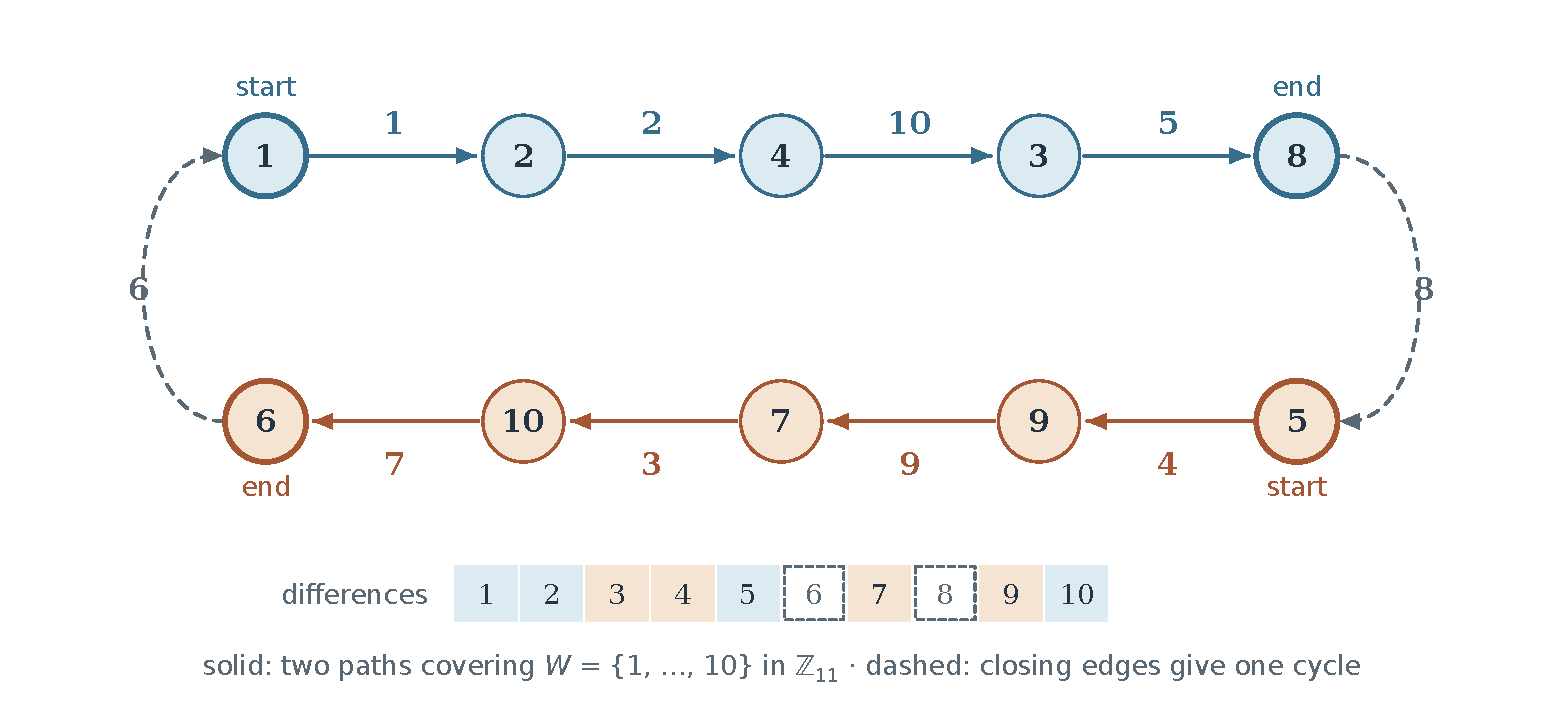
\includegraphics[width=\linewidth]{figures/fig5-paths-and-cycle.pdf}
\caption{A path factor and a cycle on \(W=\{1,\ldots,10\}\) in \(\mathbb Z_{11}\), illustrating the two forms of conclusion of Theorem 9 at small size. The solid arrows give two paths with distinct differences, initial set \(\{1,5\}\), and terminal set \(\{8,6\}\). The dashed arrows connect them into one cycle and supply the two remaining nonzero differences, \(6\) and \(8\).}
\label{fig:fig5-paths-and-cycle}
\end{figure}

Appendix B proves Theorem 9. The proof uses the near-regular hypergraph matching theorem of Alon, Kim and Spencer \cite{AKS97} and the form of Pippenger's theorem stated in \cite[Theorem 1.1]{AY05}. The appendix constructs a universal absorbing core and proves the robust fractional-matching result used to obtain uniform exact matching.

The proof fixes a common good sample before the target sets are chosen. For each exact-matching target, the exclusion set determines which vertices the absorbing core can use. We fix the core before constructing an approximate matching. The core then absorbs the small balanced zero-sum remainder left by that matching. In the path-factor construction, we install a router before the matching choices. Matchings between successive layers build paths, and we attach the leftover fragments. One exact matching closes these paths into cycles, with virtual edges added in the path case. We then set the router to merge the cycles into one. The virtual edges are then removed to recover paths with the prescribed start and end sets.

Related constructions using random matchings and prescribed endpoints appear in \cite{MP25} and \cite[Appendix A]{BBKMM25}. Bedert et al. \cite[Lemma A.1]{BBKMM25} construct paths with a prescribed pairing of their endpoints under sublinear perturbations of a layered random model. Bowtell, Montgomery, Müyesser and Pokrovskiy \cite[Section 3]{BMMP26} develop Hamilton routers in properly coloured digraphs.

Kuang and Wang \cite[Theorem 1.6]{KW26} and Nguyen, Tran and Vu \cite[Theorem 1.5]{NTV26} show that every sufficiently large set of nonzero elements of a finite abelian group admits an ordering with pairwise distinct nonempty partial sums. Javaheri \cite[Lemma 4.5]{Jav26} uses \cite{MP25} to extend partial sequencings in large groups on a square-root scale. In Theorem 9, both the near-spanning vertex set and the set of differences are prescribed. The vertex set may omit a fixed positive fraction of the group, and the construction determines the pairing between the prescribed start and end sets.

\statementstart\textbf{Proposition 9.1 (A density obstruction).} For every fixed \(\epsilon>1/4\), there are arbitrarily large odd cyclic groups in which all the hypotheses of Theorem 9 with \(K=1\) hold with \(\epsilon\) in place of \(\epsilon_0\), but the required path does not exist. This does not decide whether the boundary \(\epsilon=1/4\) is attainable.

\labelledparagraphstart\textbf{Proof.} Let \(a\geq1\), let \(b\geq0\) be even, put \(k=4a+1+3b\), \(n=3k\), and work in \(G=\mathbb Z_n\). Choose \(a\) elements of residue class two modulo three, call the set \(T\), and let \(W\) consist of \(T\) and all elements in residue classes zero and one. Take \(D=W\setminus\{0\}\), choose \(y\in T\), and set \(x=y-\sum D\). Since \(\sum D\equiv k+2a\equiv1\pmod3\), the point \(x\) lies in residue class one, hence belongs to \(W\) and is distinct from \(y\). The cardinality and endpoint-sum conditions hold.

Suppose a rainbow \(x\)-to-\(y\) path on \(W\) uses exactly \(D\). Let \(U_i\) count edges from class \(i\) to \(i+1\), and \(V_i\) those from class \(i\) to \(i-1\), with indices modulo three. Flow conservation gives \(U_0-V_1=U_2-V_0\) and \(U_1-V_2=U_2-V_0+1\). Thus the number of edges with difference one modulo three minus those with difference two modulo three is \(3(U_2-V_0)+1\). Since the path ends at a vertex of class two, \(U_2\leq a-1\), so this difference is at most \(3a-2\). The prescribed set \(D\) has \(k\) elements of class one and \(a\) of class two. The difference of the two colour counts must therefore be \(k-a=3a+1+3b\), a contradiction.

Taking \(b=0\) and letting \(a\to\infty\) gives odd orders \(n=12a+3\), with \(|W|=(3n-1)/4\). Thus exactly \((n+1)/4\) points are missing, and the missing fraction tends to \(1/4\) from above. This establishes the stated obstruction; it does not determine whether the boundary \(1/4\) is attainable. \(\square\)

\textbf{From path factors to corral diversity.} We construct a short rainbow path in \(\mathbb Z_n\) with designated middle vertices. The single-path case of Theorem 9 supplies a return path, completing a directed rotational terrace. This is a cyclic ordering of the nonzero residues in which each nonzero difference occurs once. We lift the terrace to the physical cycle and cut it into rows. Independent Latin squares then move the designated vertices within these rows, preserving the gap multisets and allowing the choices to be recovered. We use the tolerance \(\epsilon_0\) from Theorem 9.

Let \(L_r\) be the number of labelled Latin squares of order \(r\): the rows, columns and symbols are distinguished.

\statementstart\textbf{Theorem 10 (Factorial-order diversity).} Fix \(0<\epsilon\leq\min(\epsilon_0,1/100)\). For every sufficiently large height \(h\), with \(n=2h-1\) and \[
 r_*=\left\lfloor\sqrt{\frac{\epsilon n-7}{3}}\right\rfloor,
\] we have \(A_h\geq L_{r_*}^h\). Consequently, using natural logarithms, \[
 \log A_h\geq\frac{\epsilon}{3}h^2\log h-O_\epsilon(h^2),
 \qquad \log A_h=\Theta(h^2\log h).
\] The same construction also gives \(A_h\geq L_{r_{\rm old}}^h\) for \(r_{\rm old}=\lfloor\sqrt{\epsilon n/4-2}\rfloor\).

The upper order follows from Theorem 8. We give the lower-bound deduction here; Theorem 9 supplies the required path completion. No numerical first height is asserted.

\hypertarget{a-rainbow-prefix-with-latin-centres}{%
\subsection{A rainbow prefix with Latin centres}\label{a-rainbow-prefix-with-latin-centres}}

Fix an integer \(r\geq3\) and odd \(n\geq200r^2\). We construct the following explicit prefix.

\hypertarget{an-explicit-ordering-of-the-columns}{%
\subsubsection{An explicit ordering of the columns}\label{an-explicit-ordering-of-the-columns}}

Put \(R=r^2\), and let \(m\) be the least even integer at least \(r\), so \(m=r\) for even \(r\) and \(m=r+1\) for odd \(r\). For \(0\leq t<r\) define

\[
w_t=\begin{cases}
t/2,&t\text{ even},\\
m-1-(t-1)/2,&t\text{ odd}.
\end{cases}
\]

These are the first \(r\) entries of the Walecki ordering \(0,m-1,1,m-2,\ldots\) on \(\mathbb Z_m\). Define

\begin{equation}
c=\begin{cases}
0,&r\equiv0,1\pmod4,\\
(r+2)/4,&r\equiv2\pmod4,\\
(r+1)/4,&r\equiv3\pmod4,
\end{cases}
\qquad u_t=(w_t+c)\bmod m\in\{0,\ldots,m-1\}.
\tag{L4}\label{eq:L4}
\end{equation}

The column \emph{index} is \(t\in \{0,\ldots ,r-1\}\). The coordinate \(u_t\) is a distinct element of \(\{0,\ldots ,m-1\}\) and need not be below \(r\) when \(r\) is odd.

\statementstart\textbf{Column-order lemma.} The \(r-1\) differences \(\delta _t=u_{t+1}-u_t\), interpreted as ordinary integers, have distinct nonzero residues modulo \(m\). In addition, the ordinary boundary difference \begin{equation}
\delta_B=u_0-u_{r-1}=-\lfloor r/2\rfloor
\tag{L5}\label{eq:L5}
\end{equation} equals exactly one of the ordinary internal differences \(\delta _t\).

\labelledparagraphstart\textbf{Proof.} Before translation, consecutive differences of the full Walecki ordering are

\[
w_{t+1}-w_t=(-1)^t(m-1-t),\qquad 0\le t\le m-2.
\]

For even \(t\) these give the odd residues \(m-1,m-3,\ldots ,1\); for odd \(t\) they give the even residues \(2,4,\ldots ,m-2\). They are all the nonzero residues modulo \(m\), exactly once. Translation modulo \(m\) preserves those residues, and taking the first \(r\) vertices preserves distinctness.

The assertion about ordinary representatives, which is essential for separating the row joins, follows from the following four substitutions. In the table \(\delta _B=\delta _{t_0}\) as integers, not just modulo \(m\).

\begin{longtable}[]{@{}lllll@{}}
\toprule\noalign{}
\(r\) & \(m\) & \(c\) & \(t_0\) & \(\delta _B=\delta _{t_0}\) \\
\midrule\noalign{}
\endhead
\bottomrule\noalign{}
\endlastfoot
\(4k\), \(k\geq 1\) & \(4k\) & \(0\) & \(2k-1\) & \(-2k\) \\
\(4k+1\), \(k\geq 1\) & \(4k+2\) & \(0\) & \(2k+1\) & \(-2k\) \\
\(4k+2\), \(k\geq 1\) & \(4k+2\) & \(k+1\) & \(2k\) & \(-(2k+1)\) \\
\(4k+3\), \(k\geq 0\) & \(4k+4\) & \(k+1\) & \(2k\) & \(-(2k+1)\) \\
\end{longtable}

Every \(t_0\) lies in \([0,r-2]\). For example, in the third case the two entries at positions \(2k,2k+1\) become \(2k+1,0\), whereas the first and last entries are \(k+1,3k+2\). Both differences are \(-(2k+1)\). The fourth case has the same two entries at \(2k,2k+1\) and the same first and last values. The first two rows follow immediately without reduction modulo \(m\). Uniqueness follows from the distinct residues already proved. \(\square\)

The translation in (L4) makes the boundary difference equal to an internal difference as an ordinary integer. In the unshifted ordering these differences can differ by \(m\), allowing a collision between join colours. Subtracting \(u_0\) in (L6) fixes the origin for the marker-to-array edge and keeps its colour below the incoming centre colours.

\hypertarget{the-prefix-and-its-rainbow-proof}{%
\subsubsection{The prefix and its rainbow proof}\label{the-prefix-and-its-rainbow-proof}}

For \(0\leq j,t<r\) set

\begin{equation}
\begin{split}
a_j&=10R+mj,\qquad b_j=50R+mj,\\
\xi_t&=20R+(m+1)(u_t-u_0),\qquad s_{jt}=(j+t)\bmod r,\\
P_{jt}&=\xi_t-a_j,\qquad C_{jt}=\xi_t+s_{jt},\qquad
N_{jt}=\xi_t+b_j.
\end{split}
\tag{L6}\label{eq:L6}
\end{equation}

Start with the eight marker vertices, using ordinary representatives, \[
n-3,n-1,2,12,n-2,10,17,18,
\] and append

\begin{equation}
(P_{00},C_{00},N_{00}),\ldots,
(P_{0,r-1},C_{0,r-1},N_{0,r-1}),
(P_{10},C_{10},N_{10}),\ldots,
(P_{r-1,r-1},C_{r-1,r-1},N_{r-1,r-1}).
\tag{L7}\label{eq:L7}
\end{equation}

Call an edge from the last vertex \(N\) of a triple to the first vertex \(P\) of the next triple a direct join. The display lists all \(3R+8\) vertices of the prefix, so there are \(3R+7\) edges.

\hypertarget{vertex-separation}{%
\subsubsection{Vertex separation}\label{vertex-separation}}

Since \(m\leq r+1\), \[
m(r-1)\le R-1,\qquad m^2-1\le R+2r\le2R
\] for \(r\geq 3\). Thus \(18R\leq \xi _t\leq 22R\), and the following loose bands suffice:

\begin{equation}
\begin{split}
P_{jt}&\in[7R+1,12R],\\
C_{jt}&\in[18R,23R],\\
N_{jt}&\in[68R,73R].
\end{split}
\tag{L8}\label{eq:L8}
\end{equation}

These three bands and the eight marker vertices are disjoint for \(r\geq 3,n\geq 200R\); all array vertices lie strictly between \(18\) and \(n-3\). For fixed \(t\), the symbols \(s_{jt}\) run through \(0,\ldots ,r-1\) as \(j\) varies, so the centre vertices fill exactly the interval \([\xi _t,\xi _t+r-1]\). Different such intervals are disjoint because distinct \(u_t\) differ by at least one and their starting coordinates differ by at least \(m+1>r-1\).

If two P vertices agree, then

\[
(m+1)(u_t-u_{t'})=m(j-j').
\]

Reducing modulo \(m\) gives \(m|(u_t-u_{t'})\); their range forces \(u_t=u_{t'}\), then \(t=t'\), then \(j=j'\). The identical argument applies to the N vertices. Hence the whole prefix is simple and avoids zero.

\hypertarget{colours-at-the-centres-and-at-the-marker}{%
\subsubsection{Colours at the centres and at the marker}\label{colours-at-the-centres-and-at-the-marker}}

The incoming and outgoing colours of a centre, as positive ordinary differences, are

\begin{equation}
a_j+s_{jt},\qquad b_j-s_{jt}.
\tag{L9}\label{eq:L9}
\end{equation}

For a fixed \(j\), these run through the blocks

\begin{equation}
[10R+mj,10R+mj+r-1],\qquad
[50R+mj-r+1,50R+mj].
\tag{L10}\label{eq:L10}
\end{equation}

The blocks for different \(j\) are disjoint because \(m\geq r\). The incoming blocks lie in \([10R,12R]\) and the outgoing blocks in \([49R,51R]\). They are disjoint from each other.

The seven marker colours are

\[
2,3,10,n-14,12,7,1.
\]

Normalization by \(u_0\) in (L6) ensures \(\xi _0=20R\), so the first join from \(18\) to \(P_{00}\) has colour \(10R-18\). For \(r\geq 3\) this is positive, larger than 12, and strictly below every incoming block. It is disjoint from all other displayed colour bands.

\hypertarget{colours-of-all-direct-joins}{%
\subsubsection{Colours of all direct joins}\label{colours-of-all-direct-joins}}

Within row \(j\) of the array the join from cell \((j,t)\) to \((j,t+1)\) has colour

\begin{equation}
J_{jt}=n-60R-2mj+(m+1)\delta_t,
\qquad0\le t<r-1.
\tag{L11}\label{eq:L11}
\end{equation}

Between the last cell of row \(j\) and the first cell of row \(j+1\), its colour is

\begin{equation}
B_j=n-60R-m(2j+1)+(m+1)\delta_B,
\qquad0\le j<r-1.
\tag{L12}\label{eq:L12}
\end{equation}

The numerical displacement is negative: every N vertex is above every P vertex by (L8). These are therefore the positive representatives modulo \(n\), and each join makes exactly one wrap.

All colours (L11)--(L12) lie in

\begin{equation}
[n-64R,n-58R].
\tag{L13}\label{eq:L13}
\end{equation}

Indeed, the \(m\) multiple in (L11) has magnitude at most \(2R-2\); the one in (L12) is also below \(2R\); and \((m+1)|\delta |\leq m^2-1\leq 2R\). The upper bound uses that the \(m\) multiples are nonpositive. For \(n\geq 200R\), this band is above \(51R\), below \(n-14\), and separated from all colours in the preceding colour bands.

It remains to prove distinctness \emph{within} (L13). Comparing two \(J\) colours modulo \(m\) cancels the common \(n-60R\); the column-order lemma then gives the same \(t\), and equality gives the same \(j\). The B colours are pairwise distinct because successive ones differ by \(2m\). If a J colour equals a B colour, their residues force \(t=t_0\) from the column-order lemma. But \(\delta _{t_0}=\delta _B\) as ordinary integers, so equality would force \[
2j=2j'+1,
\] which is impossible. All prefix colours are therefore distinct and nonzero. This proves that the prefix is rainbow. \(\square\)

\hypertarget{positive-lift}{%
\subsubsection{Positive lift}\label{positive-lift}}

Start the positive lift at \(n-3\). The eight marker vertices finish at \(2n+18\). Since \(P_{00}=10R>18\), the first triple lies at level 2. Both edges inside every triple are positive differences below \(n\), with no wrap. Every direct join makes exactly one wrap. Thus the three lifted vertices of cell \((j,t)\) are exactly

\begin{equation}
P_{jt}+(2+rj+t)n,\quad C_{jt}+(2+rj+t)n,\quad
N_{jt}+(2+rj+t)n.
\tag{L14}\label{eq:L14}
\end{equation}

The level separates into a term in \(j\) and a term in \(t\).

\hypertarget{closing-the-prefix}{%
\subsection{Closing the prefix}\label{closing-the-prefix}}

Let \(\ell=3R+8\) be the number of prefix vertices. For the return path, let \(W\) contain the nonzero residues other than the internal prefix vertices, and let \(D\) contain the nonzero differences unused by the prefix. The two prefix endpoints remain in \(W\), and \[
 |W|=n+1-\ell,\quad |D|=n-\ell=|W|-1,\quad
 \sum D=(n-3)-\operatorname{last}(\text{prefix}).
\] The sum identity holds because the nonzero residues of odd \(\mathbb Z_n\) sum to zero and the used differences telescope. If \(\ell-1\leq\epsilon_0 n\) and \(n\geq n_0\), Theorem 9 with \(K=1\) supplies a path from the last prefix vertex back to \(n-3\). Together they give a directed rotational terrace of all nonzero residues. Fix one such ordering for all subsequent Latin choices.

\hypertarget{lifting-and-physical-row-tiles}{%
\subsection{Lifting and physical row tiles}\label{lifting-and-physical-row-tiles}}

The following lemma will also be used for a different terrace in Appendix A. \autoref{fig:fig6-tiles} illustrates the two-row splice with a small terrace.

\begin{figure}[!htbp]
\centering
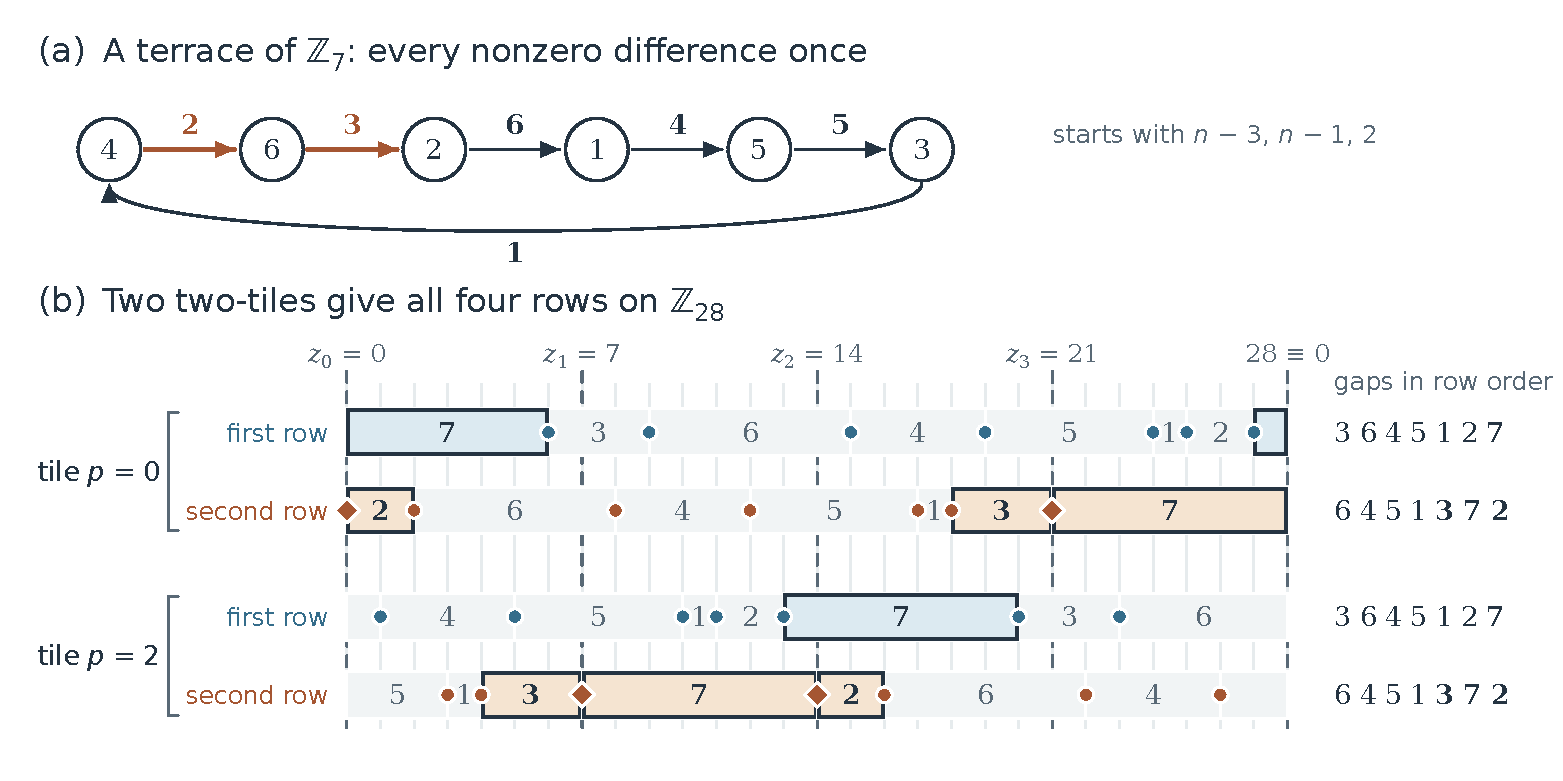
\includegraphics[width=\linewidth]{figures/fig6-tiles.pdf}
\caption{The two-row splice at \(h=4\) and \(n=7\). Lifting a directed rotational terrace in \(\mathbb Z_7\) and cutting it into two tiles gives the four physical rows on \(\mathbb Z_{28}\). The first row of each tile closes with gap \(7\). In the second row, the highlighted terrace steps of lengths \(2,3\) are replaced by connectors of lengths \(3,7,2\) through the zero sites. Each of the four rows has every gap from \(1\) to \(7\). Lemma 11 uses a longer prescribed segment to handle three-row tiles and recover the tile layout.}
\label{fig:fig6-tiles}
\end{figure}

\begin{samepage}

\statementstart\textbf{Lemma 11 (Common lift and physical tiles).} Let \(n=2h-1\geq65\), \(M=hn\). Let a \emph{directed rotational terrace}---a cyclic ordering of all nonzero residues with all nonzero differences once---start with \[
 n-3,n-1,2,12,n-2,10,17,18.
\]

\par\end{samepage}

Put \(z_p=pn\) for \(p\in\mathbb Z_h\). Starting at \(x_0=z_p+n-1\), follow the positive representatives of the terrace differences, writing the resulting physical points as \(x_0,x_1,\ldots\). For \(\ell\in\{2,3\}\), a tile starting at \(p\) consumes the sites \[
 x_0,\ldots,x_{\ell(n-1)-1},\qquad
 z_p,z_{p-1},\ldots,z_{p-\ell+1}.
\] It has \(\ell\) rows, each with gap palette \([n]\), as follows. The two-tile rows are \[
 (x_0,\ldots,x_{n-1}),\qquad
 (x_n,\ldots,x_{2n-3},z_{p-1},z_p).
\] The three-tile starts with \((x_0,\ldots,x_{n-1})\) and \((x_n,\ldots,x_{2n-1})\). Writing \(D=x_{2n}\), \(E=x_{2n+1}\) and \(Q=(x_{2n+2},\ldots,x_{3n-4})\), its third row is \[
 (D,E,z_p,Q,z_{p-2},z_{p-1}).
\] Any cyclic tiling of \(\mathbb Z_h\) by directed intervals of lengths two and three gives an optimal corral from these rows. In every row, the terrace segment from \(17\to18\) through the closing edge into \(n-3\) occurs unchanged.

For a directed gap, call its starting site its \emph{tail}. The gap-one tails of the corral are \(\{17+qn:q\in\mathbb Z_h\}\). For a two-tile starting at \(p\), its gap-two tails are \(z_p-3,z_p\) and its gap-\(n\) tails are \(z_p-1,z_{p-1}\). For a three-tile, the corresponding tails are \[
 \begin{array}{ll}
 \text{gap two:}&z_p-3,\ z_{p-1}-3,\ z_p-2,\\
 \text{gap }n:&z_p-1,\ z_{p-1}+2,\ z_{p-2}.
 \end{array}
\] After any row modifications that preserve the gap palette \([n]\) in every row and all edges of lengths \(1,2,n\), the gap-\(n\) tails distinguish the rows and the gap-two tails recover the tile layout. A physical isometry taking one such modified corral to another cannot be a reflection; any such rotation is a translation by a multiple of \(n\) that takes one recovered layout to the other. If both corrals use the same layout, with one three-tile for odd \(h\) or two consecutive three-tiles for even \(h\), that isometry is the identity.

\labelledparagraphstart\textbf{Proof.} One terrace round advances by \(1+\cdots+(n-1)=(h-1)n\equiv-n\pmod M\). Thus the lift is one cycle through all nonzero-residue sites: each residue occurs once per round and the phase decreases by one in each of the \(h\) rounds. This is the special case of \cite[Proposition 6.2]{JY26} used here. The prescribed initial segment and the displacement of a full terrace round give the following sites modulo \(M\). \begin{equation}
\begin{array}{lll}
 x_{n-1}=z_p-1,&x_n=z_p+2,&x_{2n-3}=z_{p-1}-3,\\
 x_{2n-1}=z_{p-1}+2,&x_{2n}=z_{p-1}+12,&x_{2n+1}=z_p-2,\\
 x_{2n+2}=z_p+10,&x_{3n-4}=z_{p-2}-3.
\end{array}
\tag{H3}\label{eq:H3}
\end{equation} The first row of a two-tile and the first two rows of a three-tile have all nonzero gaps internally and close with gap \(n\). The remaining two-tile segment omits gaps \(2,3\), and its new connectors have lengths \(3,n,2\). The remaining three-tile segment omits \(2,3,10\); replacing its gap \(12\) and adding the new connectors inserts \(2,10,3,n,12\). Thus every listed row has the palette \([n]\). The sites are distinct and the positive gap sum is \(n(n+1)/2=M\), so each listed order winds exactly once, including the actual wrap. Successive tiles consume consecutive nonzero segments and the corresponding disjoint zero sites, proving the partition. The cuts and the single replacement before \(17\) leave the stated terrace segment intact.

The tails in the statement follow from these same cuts and connectors. Each row has a unique gap-\(n\) tail, and different rows have different tails. Gap-two tails of residues \(0\) and \(n-2\) mark the starts of two- and three-tiles respectively; the remaining tails have residue \(n-3\). These assertions remain true when all edges of lengths \(1,2,n\) survive. For a reflection \(x\mapsto t-x\), the tail of a gap of length \(d\) maps to \(t-d-x\). Preserving the gap-one tails forces \(t\equiv35\pmod n\), but a gap-two tail of residue \(n-3\) would then map to residue \(36\), outside \(\{n-3,0,n-2\}\) for \(n\geq65\). A preserving rotation must be a multiple of \(n\), and its action on gap-two tails carries the recovered layout to the other layout. A phase translation preserving one three-tile is zero; a nonzero translation preserving two three-tile starts three phases apart must swap them and force \(h\mid6\). Since \(h\geq33\), neither fixed layout has a nonidentity symmetry. \(\square\)

For odd \(h\), use one three-tile and otherwise two-tiles. For even \(h\), use two consecutive three-tiles and otherwise two-tiles. Apply Lemma 11 to the terrace fixed in Section 8.2.

\hypertarget{independent-latin-choices}{%
\subsection{Independent Latin choices}\label{independent-latin-choices}}

For \(q\in\mathbb Z_h\), call the lift of the fixed terrace that starts at the site \(z_q+n-3\) the round of phase \(q\); by (L14), its cell \((j,t)\) lies at level \(q+2+rj+t\). Every row of Lemma 11 contains the unchanged segment through \(17\to18\); the terrace-round phase of the row is the phase of the round containing that copy of \(18\). By (H3), the rows of a tile starting at \(p\) have phases \(p\), \(p-1\) and, for a three-tile, \(p-2\), so the \(h\) rows have distinct phases. Label the physical rows by these phases \(q\in\mathbb Z_h\). By Lemma 11, every triple (L14) stays intact in its physical row. Each centre thus keeps its two neighbours from the lifted terrace.

For each \(a\in\mathbb Z_h\), choose a labelled Latin square \(S^{(a)}=(S^{(a)}_{jt})\) of order \(r\). We call the choice indexed by \(a\) a copy. Latin row \(j\) of this copy acts on the physical row of phase \(q=a-rj\). In column \(t\), replace that row's centre by \begin{equation}
Y_{a,t,S^{(a)}_{jt}},\qquad
 Y_{a,t,s}=\xi_t+s+(a+2+t)n\pmod M.
\tag{H4}\label{eq:H4}
\end{equation} Formula (L14) places the original centre at (H4) with \(s=(j+t)\bmod r\). The \(r\) rows selected by one copy are distinct: for distinct \(j,j'\), \(0<r|j-j'|\leq r(r-1)<h\), since \(n\geq200r^2\). The same physical row may occur in several copies. Their pools of selectable sites are disjoint, as verified below. \autoref{fig:fig7-latin-pools} illustrates the two Latin conditions in one copy.

\begin{figure}[!htbp]
\centering
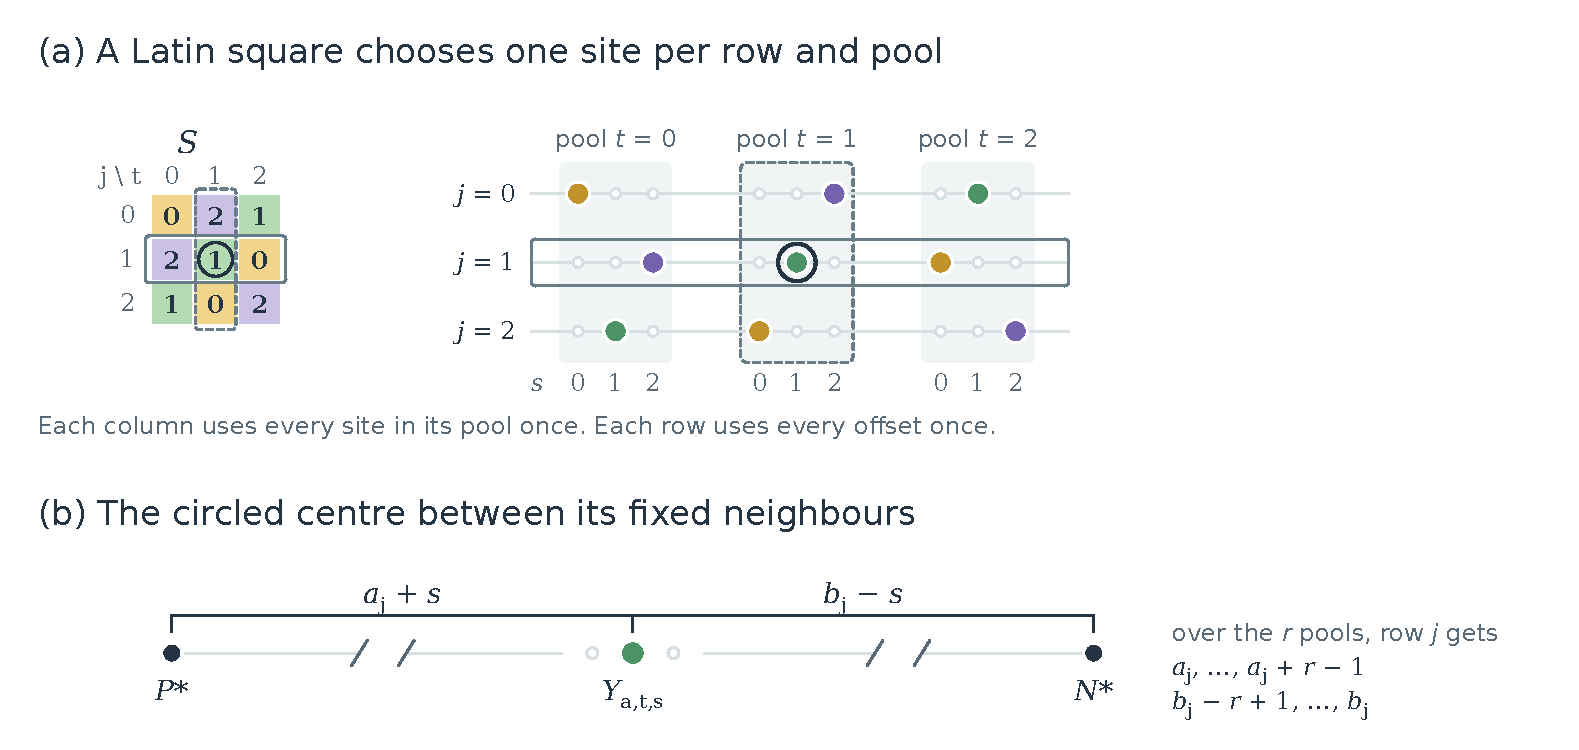
\includegraphics[width=\linewidth]{figures/fig7-latin-pools.pdf}
\caption{Schematic Latin choices in one copy with \(r=3\). The entry \(S_{jt}\) selects the offset \(s\) of row \(j\) in pool \(t\). A column uses all sites of its pool. The circled centre is shown below with its fixed neighbours \(P^*,N^*\) and gaps \(a_j+s\) and \(b_j-s\). Across the pools, a Latin row uses every offset once and supplies both complete blocks of gap lengths.}
\label{fig:fig7-latin-pools}
\end{figure}

The selectable site sets for different pairs \((a,t)\) are disjoint. Equality of two such sites first fixes \(t\) and \(s\) by the disjoint centre residue intervals, then fixes \(a\pmod h\). For each fixed \((a,t)\), the original centres on the \(r\) selected rows occupy these sites exactly once. The Latin column condition gives the same occupancy after replacement, simultaneously for all pairs. All other sites remain fixed, so the physical partition is preserved.

The new centre remains between its original neighbours in the positive lift, and its two actual gaps are \(a_j+s\) and \(b_j-s\). For a fixed row \(q\) and \(j\), the acting copy is \(a=q+rj\); its Latin row \(j\) uses every symbol once as \(t\) varies. Thus that physical row retains the complete incoming and outgoing blocks (L10), which are disjoint between different \(j\). Distinct moving centres have disjoint incident edges. Every row therefore retains its full gap palette, including the unchanged gap \(n\).

\hypertarget{decoding-symmetries-and-the-count}{%
\subsection{Decoding, symmetries and the count}\label{decoding-symmetries-and-the-count}}

The unchanged gap-\(n\) tail identifies the original phase of each unlabelled row. For a given \(a,j,t\), find the site of the row of phase \(q=a-rj\) in pool (H4). The offset of that site recovers \(S^{(a)}_{jt}\). The construction is therefore injective on the \(h\)-tuples of Latin squares.

The changed gaps lie in \([10R,12R]\cup[49R,51R]\), so they avoid \(1,2,n\) when \(n\geq200R\). Lemma 11 then shows that, for the fixed layout chosen in Section 8.3, no nonidentity physical isometry maps one family member to another. The family therefore meets exactly \(L_r^h\) asymmetric physical dihedral orbits.

For \(r=r_*\), sufficiently large \(h\) gives \(r\geq3\), \(3r^2+7\leq\epsilon n\), and \(n\geq300r^2\geq200r^2\). The prefix closes by Theorem 9. The standard labelled Latin-square bound \cite[p.~343]{MW05} gives \[
 L_r\geq\frac{(r!)^{2r}}{r^{r^2}},\qquad
 \log L_r\geq r^2\log r-2r^2.
\] For fixed \(\epsilon\), \(r_*^2=\epsilon n/3+O_\epsilon(\sqrt n)\) and \(\log r_*=\tfrac12\log n+O_\epsilon(1)\). Multiplying by \(h\) yields the lower bound of Theorem 10; Theorem 8 gives the upper order.

For \(r=r_{\rm old}\), sufficiently large \(h\) gives \(r\geq3\), \(3r^2+7\leq4r^2+8\leq\epsilon n\), and \(n\geq400r^2\). Applying the construction at this value of \(r\) proves the second bound of Theorem 10. \(\square\)

\hypertarget{constructive-software-and-formal-verification}{%
\section{Constructive software and formal verification}\label{constructive-software-and-formal-verification}}

The supplementary archive is available at \url{https://doi.org/10.5281/zenodo.24393806}.

A \href{supplement/software/construct.py}{constructor} for the explicit proof of Theorem 1 returns physical rows, permutations and shifts. A separate \href{supplement/software/verify.py}{checker} reconstructs their cyclic partial sums and tests disjointness, complete occupation and wrap gaps. Finite checks supplement the written proof. The Python implementation itself is not formally verified.

For the supplied \href{supplement/examples/height-seven.json}{height-seven certificate}, the \href{supplement/formal/README.md}{supplementary Lean check} verifies the header and array sizes, equality of the seven stored rows with the rows from Section 4.3, and the gap permutations and arrivals reconstructed from the stored shifts. A Python helper imports the JSON values into Lean.

A companion Lean development checks selected existence and counting statements. One formal proof of Theorem 9 follows the quantitative route in the written proof, with the near-regular Alon--Kim--Spencer bound and Pippenger's theorem as explicit inputs. A second formal proof derives Theorem 9 with Pippenger's theorem as its sole external matching input. The logarithmic diversity estimate additionally assumes a standard lower bound for labelled Latin squares.

The quantitative actual-remainder result is checked under its stated raw-event hypothesis and an explicit Alon--Kim--Spencer one-bite assumption; the raw-event probability and fractional-weight supplier are separately proved. The external results themselves are not proved in Lean. The \href{FORMAL-SCOPE.md}{formal-scope guide} lists the results checked in Lean and identifies the corresponding declarations and their assumptions.

\hypertarget{further-questions}{%
\section{Further questions}\label{further-questions}}

An optimal corral satisfying Nakamigawa's well-dispersed condition \cite{Nak15} is balanced. Which heights admit a balanced optimal corral?

Theorems 8 and 10 determine the order of \(\log A_h\). Can we give sharper constants and explicit height thresholds for these bounds? Can we efficiently construct the terraces with prescribed prefixes used in the diversity proof? For the path-factor theorem, how close can the universal tolerance come to the upper bound in Proposition 9.1?

\appendix

\hypertarget{an-additional-exact-family}{%
\section{An additional exact family}\label{an-additional-exact-family}}

\statementstart\textbf{Corollary A.1 (Path-to-terrace completion).} With \(\epsilon_0\) as in Theorem 9, for every sufficiently large odd \(n\), every simple directed path of \(s\) nonzero vertices in \(\mathbb Z_n\), with \(s\geq2\), \(s-1\leq\epsilon_0n\), and pairwise distinct nonzero directed differences, extends to a directed rotational terrace without changing the path.

\labelledparagraphstart\textbf{Proof.} Write the given path as \(p_1,\ldots,p_s\). Delete its internal vertices from the nonzero residues to obtain \(W\), and delete its used differences from the nonzero residues to obtain \(D\). Then \(|W|=n-s+1\), \(|D|=n-s=|W|-1\), and \(p_s,p_1\) are distinct members of \(W\). The nonzero residues sum to zero, so telescoping gives \(\sum D=p_1-p_s\). The stated bound on \(s\) gives \(|W|\geq n-\epsilon_0n\). Theorem 9 gives a return path from \(p_s\) to \(p_1\) using exactly \(W\) and \(D\). Combining it with the given path produces the required terrace. \(\square\)

Jiang and Yang \cite[Corollary 8.1]{JY26} prove terrace completion for prescribed paths of any fixed length. Their proof applies the rainbow path theorem of Müyesser and Pokrovskiy \cite[Theorem 6.9]{MP25} to the unused nonzero colours. The size condition in that theorem permits \(O(\sqrt n)\) missing vertices. In Corollary A.1, the prescribed path may have up to \(\epsilon_0 n\) edges.

\statementstart\textbf{Theorem A.2.} For every sufficiently large \(h\), put \[
 m=\left\lfloor\frac{\lfloor\sqrt{2h-1}\rfloor-8}{5}\right\rfloor.
\] Then \(A_h\geq2^{hm}\), and \(\log_2 A_h\geq(\sqrt2/5)h^{3/2}-O(h)\). Proposition A.3 gives an exact count for the larger family in which the tile layout also varies.

Throughout this appendix let \(n=2h-1\), \(M=hn\), and take \(h\) sufficiently large that Corollary A.1 applies. We also assume \(n\geq65\), so that \(m\geq0\). Identify each nonzero directed difference with its representative in \([n-1]\).

\hypertarget{a-terrace-with-prescribed-switches}{%
\subsection{A terrace with prescribed switches}\label{a-terrace-with-prescribed-switches}}

We prescribe the initial path \begin{equation}
(n-3,n-1,2,12,n-2,10,17,18),
\tag{A1}\label{eq:A1}
\end{equation} whose successive differences are \(2,3,10,n-14,12,7,1\). For \(0\leq i<m\), define \begin{equation}
\begin{aligned}
 \epsilon_i&=i\bmod2,&
 \alpha_i&=8i+20,&
 \beta_i&=8i+23+\epsilon_i,\\
 p_i&=8i^2+44i+38+\lfloor i/2\rfloor,
\end{aligned}
\tag{A2}\label{eq:A2}
\end{equation} and append the five vertices

\begin{equation}
(p_i,\ p_i+\alpha_i+1,\ p_i-\beta_i,\
   p_i+1,\ p_i+\beta_i+1).
\tag{A3}\label{eq:A3}
\end{equation}

The predecessor of the first appended vertex is \(p_i-\alpha_i\): for \(i=0\) it is \(18\), and for \(i>0\) it is the last vertex of the preceding block. Thus the five new differences are

\begin{equation}
\alpha_i,\quad \alpha_i+1,\quad
 n-(\alpha_i+\beta_i+1),\quad
 \beta_i+1,\quad\beta_i.
\tag{A4}\label{eq:A4}
\end{equation}

This prescribed path is simple and rainbow. Indeed, \(n\geq(5m+8)^2\). The low differences in block \(i\) lie in \([8i+20,8i+25]\), so these sets are pairwise disjoint and avoid the low differences of (A1). The remaining differences are \(n-(16i+44+\epsilon_i)\); they are pairwise distinct, avoid \(n-14\), and exceed all the low differences because \(n>24m+46\). Since \(n\geq(5m+8)^2\), the difference \(n-14\) also exceeds every low difference.

For the vertices, (A1) is simple at \(n\geq65\). The first backward vertex in (A3) is \(15\), distinct from the low vertices of (A1). For \(i>0\), write \(E=p_i-\alpha_i\) for the preceding endpoint. The new backward vertex is \(E-3-\epsilon_i\), whereas the only previous block vertex immediately below \(E\) is \(E-3-\epsilon_{i-1}\); these differ because the parities alternate. Every other earlier low vertex is at most \(p_{i-1}+1\), at least 19 below the new backward vertex. The other four vertices of the new block are distinct and greater than \(E\); for \(i=0\) they are \(38,59,39,62\), all greater than \(18\). Finally, the greatest low vertex in all appended blocks, when \(m>0\), is

\[
 8m^2+36m+18+\lfloor m/2\rfloor<n-3.
\]

They therefore avoid the three high vertices \(n-3,n-2,n-1\) in (A1). All prescribed vertices are nonzero. The path has \(5m+8\leq\sqrt n\) vertices, and \(\sqrt n-1\leq\epsilon_0n\) for sufficiently large \(n\). Corollary A.1 therefore supplies a terrace containing the path. Fix one such terrace for the rest of this section.

\hypertarget{two--and-three-row-tiles}{%
\subsection{Two- and three-row tiles}\label{two--and-three-row-tiles}}

Apply Lemma 11 to this terrace and to any cyclic tiling of \(\mathbb Z_h\) by directed intervals of lengths two and three. The resulting rows form an optimal corral. The terrace continuation after \(18\) stays intact in each row, and the gap-one, gap-two and gap-\(n\) tails have the marker properties of Lemma 11.

\hypertarget{independent-local-switches}{%
\subsection{Independent local switches}\label{independent-local-switches}}

The part of the terrace after the vertex \(18\), including every block (A3), occurs once and unaltered in each tile row. Fix a block \(i\) and a phase \(q\), and put

\[
 x=p_i+qn,\qquad y=x+1\pmod M.
\]

The row containing \(x\) has the incoming and outgoing gap lengths \((\alpha_i,\alpha_i+1)\). The row containing \(y\) has the lengths \((\beta_i+1,\beta_i)\). These are different rows: between the two centers \(p_i\) and \(p_i+1\) in the terrace continuation, the positive displacement is

\[
 (\alpha_i+1)+n-(\alpha_i+\beta_i+1)+(\beta_i+1)=n+1.
\]

Thus the second center in the row of \(x\) is \(x+n+1\), not \(y\). Exchange the owners of the adjacent sites \(x,y\). At the first row's center, the two gaps become \((\alpha_i+1,\alpha_i)\); at the second they become \((\beta_i,\beta_i+1)\). Each row keeps its gap multiset, and every physical site remains occupied exactly once.

All \(mh\) switches may be chosen independently and applied simultaneously. In each row the four support colors of a block are distinct, and the support colors of different blocks are disjoint. Since each color appears only once in a row, no two switches use the same old edge there. Moreover, simplicity of the prescribed path ensures that no moving center is a fixed neighbor of another moving center. Accordingly the local gap reversals do not interfere.

For a fixed tile layout, different switch sets give different unordered partitions. Each original row has one directed gap of length \(n\). The switches change only their old support edges, all of whose lengths are less than \(n\); hence each gap-\(n\) edge survives in its original row. Its tail is a distinct physical site, so it identifies which original row became each unlabelled row of the new partition. The owner of either centre site then recovers its switch. Thus there are \(2^{mh}\) different partitions for each fixed layout.

\hypertarget{physical-markers-and-proof-of-theorem-a.2}{%
\subsection{Physical markers and proof of Theorem A.2}\label{physical-markers-and-proof-of-theorem-a.2}}

The switch support gaps are at least \(20\) and smaller than \(n\), so the switches preserve every edge of lengths \(1,2,n\). Use the layout of Lemma 11 with one three-tile for odd \(h\), or two consecutive three-tiles for even \(h\). The lemma recovers this layout from the gap-two tails and excludes every nonidentity physical isometry between members of the family. Each of the \(2^{mh}\) switch sets yields an asymmetric partition, and distinct switch sets are not related by a physical isometry. Hence \(A_h\geq2^{mh}\). The estimate for \(\log_2 A_h\) follows from \(m=(\sqrt{2h-1}/5)+O(1)\). This proves Theorem A.2. \(\square\)

\hypertarget{counting-the-constructed-family}{%
\subsection{Counting the constructed family}\label{counting-the-constructed-family}}

The constructed family of this section lets the layout vary as well: it consists of the partitions obtained from Lemma 11 and the switches of Section A.3 for every cyclic tiling of \(\mathbb Z_h\) by directed intervals of lengths two and three and every switch set. Let \(C_j\) be the number of tilings of the labelled directed cycle \(\mathbb Z_j\) by intervals of lengths two and three. For \(j\geq1\),

\begin{equation}
C_j=\sum_{2a+3b=j}\frac{j}{a+b}\binom{a+b}{a}.
\tag{A8}\label{eq:A8}
\end{equation}

Set \(Q=2^m\). For the next statement \(m\) is the value chosen at the actual height \(h\); it is not recomputed at divisors of \(h\).

\statementstart\textbf{Proposition A.3 (Exact family counts).} The constructed family contains exactly \begin{equation}
\frac1h\sum_{d\mid h}\varphi(d)C_{h/d}Q^{h/d}
\tag{A9}\label{eq:A9}
\end{equation} physical equivalence classes, of which exactly \begin{equation}
\frac1h\sum_{d\mid h}\mu(d)C_{h/d}Q^{h/d}
\tag{A10}\label{eq:A10}
\end{equation} are asymmetric. Here \(\varphi\) and \(\mu\) are Euler's totient and Möbius functions. If \(\lambda>1\) is the real root of \(\lambda^3=\lambda+1\), the number in (A10) is \((\lambda Q)^h(1+o(1))/h\). Consequently

\[
 \log_2 A_h\geq mh+(\log_2\lambda)h-\log_2 h-o(1).
\]

\labelledparagraphstart\textbf{Proof.} For (A8), count tilings with one marked tile: choose one of the \(\binom{a+b}{a}\) sequences of \(a\) two-tiles and \(b\) three-tiles read from the marked tile, and place its start at one of the \(j\) labelled phases. Each tiling with \(a+b\) tiles arises \(a+b\) times.

The gap-two markers recover the layout of every partition in the family. For that layout the gap-\(n\) tails identify the rows, and the owners of the exchanged sites recover the switch bits. The \(m\) bits at each phase give exactly \(C_hQ^h\) physical partitions. Translation by \(tn\) shifts each tile and its switch bits by \(t\) phases, preserving the bit values. By Lemma 11, physical equivalence inside this family is precisely this cyclic action.

A shift of the \(h\) phases with \(j=\gcd(h,t)\) cycles fixes precisely \(C_jQ^j\) decorated layouts. Burnside's lemma gives (A9). Möbius inversion counts those with least period \(h\); dividing by \(h\) gives (A10), since those and only those have trivial rotational stabilizer and no member has a reflection symmetry.

For the asymptotic, the directed state graph with transitions \(0\to1\to0\) and \(0\to1\to2\to0\) encodes the two tile sizes. Its adjacency matrix \[
 B=\begin{pmatrix}0&1&0\\1&0&1\\1&0&0\end{pmatrix}
\] satisfies \(C_j=\operatorname{tr}(B^j)\) and has characteristic polynomial \(x^3-x-1\). Thus \(C_j=\lambda^j+o(\lambda^j)\). In (A10), the proper-divisor terms have total magnitude \(O(h(\lambda Q)^{h/2})\), uniformly for \(Q\geq1\). The asserted asymptotic follows. \(\square\)

\hypertarget{near-spanning-paths-cycles-and-factors}{%
\section{Near-spanning paths, cycles and factors}\label{near-spanning-paths-cycles-and-factors}}

This appendix proves Theorem 9. Section B.1 states the uniform exact-matching theorem. Section B.2 constructs a core that can absorb any permitted small remainder, and Section B.3 bounds the remainder left by a matching outside that core. Section B.4 combines these two results. Section B.5 supplies the matchings between successive layers. Section B.6 uses those matchings, the router and one exact matching to assemble the path factor. All groups are finite and abelian. Order thresholds in the odd-order results are uniform over the group. \autoref{fig:fig8-roadmap} follows the choices in the proof and the use of Theorem 9 in Section 8.

\begin{figure}[!htbp]
\centering
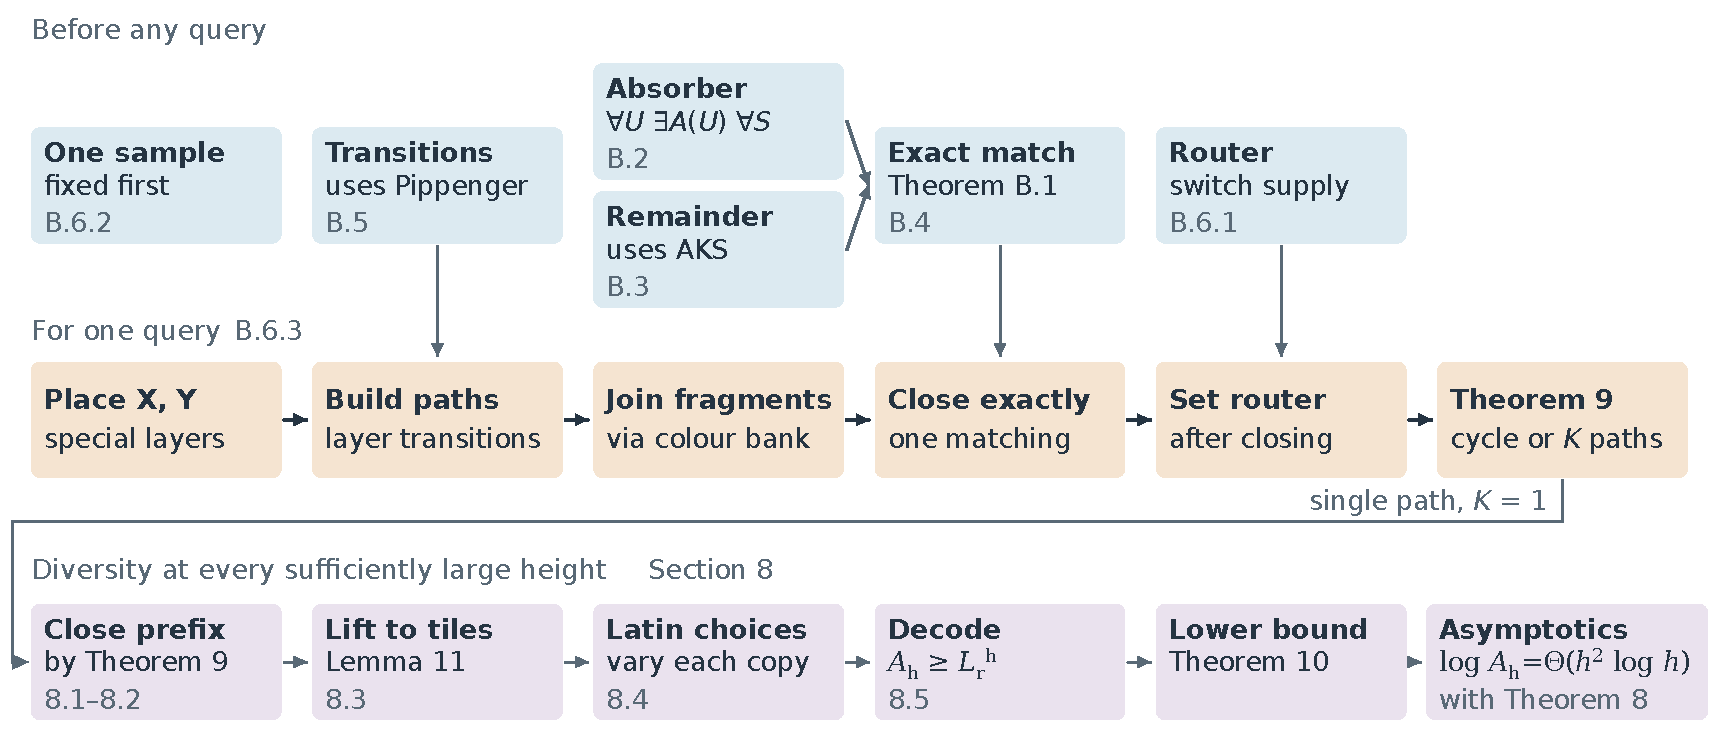
\includegraphics[width=\linewidth]{figures/fig8-roadmap.pdf}
\caption{The proof of Theorem 9 and its application to diversity. The top row lists the guarantees of one common sample for all later queries. Each query determines the paths, the fragment joins and the closing matching. The router is installed before that matching and set afterwards. The single-path case \(K=1\) closes the prefix used to construct and count the corral family in Section 8.}
\label{fig:fig8-roadmap}
\end{figure}

\hypertarget{uniform-exact-matching-and-its-inputs}{%
\subsection{Uniform exact matching and its inputs}\label{uniform-exact-matching-and-its-inputs}}

For \(f:G\to\mathbb C\) and a character \(\chi\), write \(\widehat f(\chi)=\sum_{x\in G}f(x)\overline{\chi(x)}\) for the unnormalised Fourier transform, and \((f*g)(x)=\sum_{y\in G}f(y)g(x-y)\) for convolution. We use character orthogonality and Parseval, Hall's theorem, and standard Chernoff, Hoeffding and bounded-differences inequalities with their stated independence assumptions.

\begin{samepage} We use Pippenger's near-perfect matching theorem in the form stated by Alon and Yuster, Theorem 1.1: for every integer \(r\ge2\) and \(t>0\), there is \(\mu=\mu(r,t)>0\) such that an \(r\)-uniform hypergraph \(H\) with positive maximum degree and \begin{equation}
\delta(H)\ge(1-\mu)\Delta(H),\qquad \Delta_2(H)<\mu\Delta(H)
\tag{PB1}\label{eq:PB1}
\end{equation} has a matching leaving at most \(t|V(H)|\) vertices uncovered. Here \(\delta,\Delta,\Delta_2\) denote minimum degree, maximum degree and maximum codegree. \par\end{samepage}

For each fixed t, choose a positive \(\mu_t\le\min\{1/2,\mu(3,t/2)\}\) from Pippenger's theorem. Put \(\phi_P(d_0,t)=\min\{d_0^2/10^6,t/12,\mu_t d_0^2/20\}\). No monotonicity of \(\mu_t\) in \(t\) is assumed.

\statementstart\textbf{Theorem B.1 (uniform exact matching).} Fix a real number \(0<q\leq 1/2\). At each element of a finite abelian group \(G\), independently assign a label \(1,2,*\) with probabilities \(q,q,1-2q\), and let \(R_1,R_2\) be the first two classes. Independently of this vertex process, let \(R_3\) be a Bernoulli-\(q\) subset of \(G\). Define

\begin{equation}
\begin{gathered}
\eta=10^{-4},\qquad \rho=(\eta q)^2/9,\qquad p=\rho/4,\qquad
\tau=10^{-30}p^4,\qquad \kappa=10^{-30}\tau^9,\\
\delta_{\rm BM}=10^{-6}\kappa
 =10^{-306}(10^{-8}/36)^{36}q^{72},\\
r_0=\eta q/2,\qquad \xi=\kappa r_0/10^6,\qquad
t_E=\kappa/10^5,\\
\lambda_E=\min\{\xi,\phi_P(r_0,t_E)\},\qquad
c_{\rm exp}=\lambda_E^4/10^6.
\end{gathered}
\tag{ME1}\label{eq:ME1}
\end{equation}

There is an integer \(n_0(q)\), independent of the isomorphism type of \(G\), such that, if \(|G|=n\geq n_0(q)\) is odd, with probability at least \(1-\exp(-c_{\rm exp}n)\) the following holds simultaneously for every triple \(X,Y,Z\subseteq G\): if \begin{equation}
\begin{gathered}
X\cap Y=\varnothing,\qquad 0\notin Z,\qquad |X|=|Y|=|Z|,\\
|X\triangle R_1|+|Y\triangle R_2|+|Z\triangle R_3|
 \leq\delta_{\rm BM}n,\qquad
\sum Z=\sum Y-\sum X,
\end{gathered}
\tag{ME2}\label{eq:ME2}
\end{equation} then there is a bijection \(f:X\to Y\) for which \(\{f(x)-x:x\in X\}=Z\), with every element of \(Z\) occurring once. The triple may be selected after inspecting all the samples and all the auxiliary randomness introduced in the proof. No numerical value of \(n_0(q)\) is supplied here.

We use three tagged copies \(G_A,G_B,G_C\), and put an edge on \((a,b,c)\) exactly when \(a+b+c=0\). Tags distinguish vertices with equal numerical coordinates. A tagged set is \emph{balanced} if its three part sizes are equal, and is \emph{zero-sum} if the sum of all its coordinates is zero. It is \emph{nonzero} if it contains no vertex whose coordinate is zero; this convention includes the empty set. Write \(\pi(D)\subseteq G\) for the numerical coordinate projection of a tagged set \(D\), and \(\operatorname{cl}(F)=F\cup(-F)\) for numerical inverse closure. Thus \(|\operatorname{cl}(\pi(D))|\leq2|D|\).

The signed samples and targets are

\begin{equation}
(R_A,R_B,R_C)=(-R_1,R_2,-R_3),\qquad
(X_A,X_B,X_C)=(-X,Y,-Z).
\tag{ME3}\label{eq:ME3}
\end{equation}

Write \(R=R_A\sqcup R_B\sqcup R_C\) for their tagged union. Negating the coordinates in two roles preserves the symmetric-difference distance in (ME2). The original sampled start and end sets are disjoint, so \((-R_A)\cap R_B=\varnothing\). An exact matching on the signed targets proves the theorem, since \(-x+y-z=0\) is precisely \(z=y-x\).

The proof is in Section B.4. The core is selected after the exclusion set and before the later matching remainder; that proof also gives the joint-event and projection argument.

\hypertarget{two-quantitative-ingredients}{%
\subsubsection{Two quantitative ingredients}\label{two-quantitative-ingredients}}

We record two results used by the exact-matching proof. The complete statements, probability constructions and proofs are in Sections B.2--B.3; the finite-group thresholds are uniform over the specified group types.

\statementstart\textbf{Universal absorbing core.} Use the odd-order sampling model and parameters of Theorem B.1, and put \(\widehat\kappa=10^{-6}\tau^2\). Split each signed sample into its minus and plus parts by independent coin flips on the sampled vertices, as described in Section B.2. For all \(n\) above a q-dependent threshold, there is one event of the augmented sample, failing with probability at most \(C n^7e^{-\tau^{24}n/16000}\), such that, for every later numerical set \(U\subseteq G\) of size at most \(\widehat\kappa n\), there is a nonzero tagged set \(A\) in the signed raw minus parts, numerically avoiding \(U\), with \(|A|<16200\tau n\). This same \(A\) admits a perfect matching on \(A\sqcup S\) for every later nonzero, balanced, zero-sum tagged \(S\), disjoint from \(A\), of size at most \(\widehat\kappa n\). Taking \(S=\varnothing\) makes \(A\) itself matchable. The order of choices is one event, then \(U\), then \(A\), then \(S\).

\statementstart\textbf{Robust fractional matching.} Fix \(0<q\le1/2\) and use the categorical endpoint and independent colour sampling law of Theorem B.1, in any finite abelian group. Fractional perfect weights are nonnegative edge weights whose sum at each vertex is one. On a single event with failure at most \(18n\exp(-q^8n/(4\cdot10^{10}))\), every later triple of equal size \(m\), with nonzero colours and total symmetric-difference distance at most \(q^2n/10000\) from the raw samples, has fractional perfect weights on its allowed difference edges in \([1/(2qm),3/(2qm)]\), even after deleting any edge family of maximum tagged vertex degree at most \(q^2n/2000\). No checksum or endpoint disjointness is required. See Section B.3 for the fractional proof and actual-remainder theorem. The edge-deletion conclusion is fractional: it is not an edge-deletion guarantee for the ordinary universal absorber.

The same matching module proves an actual near-matching with at most \(O(\sqrt n\log^{3/2}(en))\) uncovered tagged vertices on each admissible physical target. Its proof applies the near-regular theorem of Alon--Kim--Spencer after bounded-error degree rounding; the exact completion then uses the preselected core. For that application the preselected matching and edge ban in the stronger remainder statement are empty. The fractional and remainder results retain their full stated hypotheses and conclusions.

\hypertarget{universal-absorbing-core}{%
\subsection{Universal absorbing core}\label{universal-absorbing-core}}

This section proves the quantitative universal core used in Theorem B.1. Its core lies in the specified raw minus parts and its residual and numerical-exclusion scales are quadratic in the Q density. Throughout this section, G is a finite abelian group of odd order n.

\hypertarget{model-and-construction}{%
\subsubsection{Model and construction}\label{model-and-construction}}

Use the categorical samples, signed tagged model and constants from Theorem B.1 and (ME1). In particular, \(0<q\leq1/2\) is fixed and \(G\) has odd order \(n\). The absorber below has fewer than \(16200\tau n\) vertices and handles up to \(\widehat\kappa n=10^{-6}\tau^2 n\) later residual vertices; its permitted numerical exclusion has the same scale. Both are positive fixed fractions for fixed \(q\), and the residual capacity can be far smaller than the core itself.

\hypertarget{the-robust-template-and-probability-tools}{%
\subsubsection{The robust template and probability tools}\label{the-robust-template-and-probability-tools}}

\statementstart\textbf{Lemma B.2 (elementary bounded-degree selection graph).} For every integer \(s\ge 1\) there is a simple bipartite graph H with classes \(D\) and \(F\sqcup W\), \(|D|=3s\), \(|F|=|W|=2s\), maximum degree at most 16, such that every \(s\)-subset \(W_0\subseteq W\) gives a perfect matching between \(D\) and \(F\sqcup W_0\). In particular the later argument can take \(s_0=1\) and use the convenient degree-100 upper bound below.

\labelledparagraphstart\textbf{Proof.} Split D into three blocks \(D_1,D_2,D_3\) of size s and split the right side into four blocks \(F_1,F_2,W_1,W_2\), each of size s. Between each left block and each right block independently place four uniformly random perfect matchings. Repeated edges are merged. Left degrees are at most 16 and right degrees at most 12.

It suffices that the following two properties hold:

\begin{equation}
\begin{array}{ll}
\text{(L)}& |N_F(A)|\ge |A|\quad\text{for every }A\subseteq D,\ |A|\le s,\\
\text{(R)}& |N_D(B)|\ge |B|\quad\text{for every }B\subseteq F\sqcup W,\ |B|\le2s.
\end{array}
\tag{T1}\label{eq:T1}
\end{equation}

Here and below neighborhoods are taken in H. To prove sufficiency, fix \(W_0\) and \(A\subseteq D\), writing \(a=|A|\). If \(a\le s\), property (L) gives Hall's inequality inside F alone. If \(a>s\) and more than \(3s-a\) right vertices have no neighbor in A, choose \(B\) of exactly \(3s-a+1\le 2s\) such vertices. Then \(N_D(B)\subseteq D\setminus A\) has size at most \(3s-a<|B|\), contradicting (R). Hence

\[
|N_{F\sqcup W}(A)|\ge a+s.
\]

Deleting the s vertices \(W\setminus W_0\) leaves at least a neighbors. Hall's theorem gives a matching covering D. Both selected sides have size \(3s\), so it is perfect. This argument applies to every \(W_0\) on the same graph.

We now bound the probabilities of failures of (L) and (R). For a uniform perfect matching between two s-element blocks and fixed subsets of sizes x,y, the probability that the image of the first subset lies in the second is \begin{equation}
\frac{\binom yx}{\binom sx}\le(y/s)^x,
\tag{T2}\label{eq:T2}
\end{equation} with probability zero when \(x>y\). The harmless convention \(0^{0}=1\) handles empty subsets.

Fix \(A\subseteq D\) with \(|A|=a\le s\) and \(T\subseteq F\) with \(|T|=a-1\). Write the two F-block intersections of T as \(t_1,t_2\). Independence between the block matchings and (T2), followed by the arithmetic-geometric mean inequality, give

\[
\Pr(N_F(A)\subseteq T)
\le \bigl(t_1t_2/s^2\bigr)^{4a}
\le \left(\frac{a}{2s}\right)^{8a}.
\]

Since \(a\le s\), \(\binom{2s}{a-1}\le \binom{2s}{a}\). Using \(\binom{N}{j}\le (eN/j)^j\), a union bound therefore gives

\begin{equation}
\Pr(\text{L fails})
\le\sum_{a=1}^{s}
\left[\frac{6e^2}{2^8}\left(\frac as\right)^6\right]^a.
\tag{T3}\label{eq:T3}
\end{equation}

For (R), fix \(B\subseteq F\sqcup W\), \(|B|=b\le 2s\), and a proposed containing set \(A\subseteq D\), \(|A|=b-1\). Write \(a_i=|A\cap D_i|\). Apply (T2) to the inverse block matchings. Independence gives

\[
\Pr(N_D(B)\subseteq A)
\le\left(\frac{a_1a_2a_3}{s^3}\right)^{4b}
\le\left(\frac{b}{3s}\right)^{12b}.
\]

The exact ratio \[
\frac{\binom{3s}{b-1}}{\binom{3s}b}
=\frac b{3s-b+1}\le2
\] holds for \(b\le 2s\). Thus

\begin{equation}
\Pr(\text{R fails})
\le2\sum_{b=1}^{2s}
\left[3e^2\left(\frac23\right)^{12}
       \left(\frac b{2s}\right)^{10}\right]^b.
\tag{T4}\label{eq:T4}
\end{equation}

The elementary bound \(e^{2}<37/5\) gives

\[
\frac{6e^2}{2^8}<\frac7{40},\qquad
3e^2\left(\frac23\right)^{12}<\frac7{40}.
\]

Discarding the factors \((a/s)^{6}\) and \((b/(2s))^{10}\), and extending both sums to infinity, bounds the probability of either failure by

\begin{equation}
3\sum_{j\ge1}(7/40)^j=\frac7{11}<1.
\tag{T5}\label{eq:T5}
\end{equation}

Some graph therefore satisfies (T1), proving the lemma. This is an existence proof for a deterministic graph; its auxiliary probability does not become a failure term in the group sample. \(\square\)

We use Hall's theorem, character orthogonality, Parseval, Markov's and Chebyshev's inequalities, and the following standard concentration bounds: for independent Bernoulli variables with sum of means \(\mu\), the lower half-mean tail is at most \(e^{-\mu/8}\); for \(N\) independent variables of range length at most one, a two-sided deviation by \(t\) has probability at most \(2e^{-2t^2/N}\); and for a function of independent variables whose coordinate changes are bounded by \(c_i\), the corresponding two-sided tail is at most \(2e^{-2t^2/\sum c_i^2}\). These background inequalities are used with their independence hypotheses specified at each application.

\hypertarget{algebra-and-the-coupled-reservoirs}{%
\subsubsection{Algebra and the coupled reservoirs}\label{algebra-and-the-coupled-reservoirs}}

\statementstart\textbf{Lemma B.3 (reservoir law).} The signed samples admit a coupled augmentation with raw minus and plus parts, of respective marginal densities \(\eta q\) and \(d=(1-\eta)q\), and nonzero paired reservoirs \(V,P,Q\) with the following properties. Each reservoir is contained in the raw minus parts. On each nonzero inverse orbit \(\{g,-g\}\), the part labels of \(V\) are categorical, with probability \(\rho\) for each specified part. The six labels \(P_A,P_B,P_C,Q_A,Q_B,Q_C\) are categorical, with probabilities \(p,p,p,\tau,\tau,\tau\). Different inverse orbits have independent labels. Moreover \(P\cup Q\subseteq V\), and the numerical supports of \(P,Q\), including across different parts, are disjoint.

\labelledparagraphstart\textbf{Proof.} Multiplication by two is an automorphism of an odd-order abelian group: its kernel has no nonzero element, so finiteness gives surjectivity. Every nonzero inverse orbit consequently has two elements. An affine equation in \(e\) group variables with some coefficient \(\pm1\) or \(\pm2\) has exactly \(n^{e-1}\) solutions, since fixing the other variables determines that variable uniquely. We will use this fact in place of vector-space rank arguments.

Thin each sampled part using independent coins: retain probability \(\eta\) as minus and the remainder as plus. At an original vertex coordinate the refined probabilities for the two parts are \(\eta q,d,\eta q,d,1-2q\); only one label is present. The colour process is independent. Independence holds across original coordinates, although minus and plus in the same part are disjoint and dependent.

Independently on each nonzero inverse orbit, propose one of the three parts uniformly. If both coordinates lie in that part's raw minus class, accept with a further independent probability \(1/3\). The probability of acceptance into any specified part is \((1/3)(\eta q)^2(1/3)=\rho\). Only one proposal was made, so these labels are categorical. Different orbits inspect disjoint original coordinates and independent coins. Label each accepted orbit as P with probability \(p/\rho\), Q with probability \(\tau/\rho\), and neither otherwise. This proves every asserted law. The probabilities are valid because \(p=\rho/4\) and \(\tau\ll p\). Nothing requires \(1-2q>0\), so \(q=1/2\) is allowed. The parent \(V\) only couples P and Q; it is not used later. \(\square\)

All subsequent random choices can be put in a finite joint probability space before any target is queried. No independence of these augmentations from a later target will be assumed.

\hypertarget{packed-availability-and-selectors}{%
\subsubsection{Packed availability and selectors}\label{packed-availability-and-selectors}}

\statementstart\textbf{Lemma B.4 (uniform packed availability).} Fix \(m\geq1\) and \(C_0\) independently of \(n\). For each admissible bounded root query, specify a nonempty list of \(r\leq m\) affine forms in \(e\geq1\) free parameters, representing the new inverse orbits of a candidate gadget. Each individual form has a coefficient \(\pm1\). Include every zero, signed pair and signed root collision. Suppose each such test is either excluded by the root hypotheses or has a coefficient \(\pm1\) or \(\pm2\), with at most \(C_0\) tests remaining. An assignment is valid when it avoids these tests; any other required gadget identities hold for every valid assignment.

There are at least \(n^e-C_0n^{e-1}\) valid assignments. Forbidding one old inverse orbit removes at most \(2mn^{e-1}\) assignments. After \(i\) packed candidates, at most \(2m^2i n^{e-1}\) additional assignments are excluded. Consequently one can first fix linearly many distinct, orbit-disjoint candidates in each of polynomially many root queries, with the same bounds \(m,C_0\) throughout.

For each candidate, prescribe before sampling at most one categorical reservoir label on each of any of its new orbits. Fix \(0<v\leq1\) independently of \(n\), and suppose every prescribed label has probability at least \(v\). Different inverse orbits receive independent labels. One event of exponentially high probability then gives linearly many successful candidates in every query. On that event every later forbidden numerical set smaller than the successful count for that query can be avoided by a successful candidate's full new orbit support.

\labelledparagraphstart\textbf{Proof.} The affine counting fact in Lemma B.3 bounds each collision equation by \(n^{e-1}\); a union bound is an upper bound even when these equations overlap. To hit an old orbit, one of the new representatives must equal one of its two signs, giving at most \(2m\) equations. Previously packed candidates reserve at most \(mi\) orbits. Whenever the resulting upper bound on excluded assignments is less than \(n^e\), another candidate exists. Fix a deterministic choice rule before sampling.

A valid candidate inspects different orbit labels and has probability at least \(v^m\) of success. The candidates in its packed family inspect disjoint orbits, so their success indicators are independent. Chernoff, followed by the polynomial root-query union bound, proves the asserted common event. Afterwards each forbidden coordinate can meet at most one candidate in that query's packed family. Thus at most the cardinality of the forbidden set successful candidates are destroyed, regardless of its dependence on the samples or earlier constructions. There is no union bound over forbidden sets. \(\square\)

For the following four-orbit primitives, take \(C_0\leq40\) and pack \(\lfloor n/1000\rfloor\) candidates. Indeed \(2\cdot4^2/1000=0.032<1\). For sufficiently large \(n\), the mean number of successes is at least \(p^4n/2000\). The common event supplies at least \(p^4n/4000\) successes per query, with per-query failure at most \(e^{-p^4n/16000}\). We reserve the smaller capacities

\begin{equation}
C_{P,0}=p^4n/10^{10},\qquad C_P=p^4n/10^{12}.
\tag{AC5}\label{eq:AC5}
\end{equation}

\statementstart\textbf{Lemma B.5 (coloured selectors).} On that event, any \(1\leq k\leq100\) distinct nonzero inverse pairs in one tagged part have an interior \(I\subseteq P\) of at most \(18k-2\leq1798\) tagged vertices such that for each target pair \(T_i\) there is a matching on exactly \(I\sqcup T_i\). The same interior works for every choice of \(i\). It can avoid any later external numerical support of size at most \(C_P\), provided \(n\) is large enough that \(4000<C_{P,0}-C_P\). The root pairs need not lie in P.

\labelledparagraphstart\textbf{Proof.} It suffices to describe one part rotation, with targets in A. For two distinct nonzero inverse pairs \(\{\pm a\},\{\pm b\}\), put four interior vertices at

\begin{equation}
B:u,\ u+a+b;\qquad C:-a-u,\ -b-u.
\tag{AC6}\label{eq:AC6}
\end{equation}

The two states consist of the edges

\begin{equation}
\begin{array}{ll}
(a,u,-a-u),&(-a,u+a+b,-b-u),\\
(b,u,-b-u),&(-b,u+a+b,-a-u).
\end{array}
\tag{AC7}\label{eq:AC7}
\end{equation}

Each row matches the same interior and its indicated target pair. Each edge has sum zero. Among the four affine representatives there are four zero equations, twelve signed pair comparisons and sixteen signed root comparisons, at most 32 equations. Parameter-free failures would force one of \(a,b,a+b,a-b\) to vanish, contrary to the root hypotheses; every remaining equation has coefficient \(\pm1\) or \(\pm2\). All four new orbits can therefore be required to be distinct and fresh.

For \(1\leq k\leq3\), use a common B pair \(\{\pm u\}\) and the C pairs \(\{\pm(a_i+u)\}\). If target i is chosen, its two edges are \((a_i,u,-a_i-u)\) and \((-a_i,-u,a_i+u)\). This star uses at most four new orbits. Its at most four zero equations, twelve signed pair comparisons and 24 signed root comparisons give \(C_0\leq40\). The only parameter-free failures assert that a target is zero or two target pairs are the same; all other coefficients are \(\pm1\) or \(\pm2\). Between each two consecutive C pairs install a fresh switch of (AC6). To select i, switches before i take their left pair and switches at or after i take their right pair. The star covers the unique remaining C pair and the chosen A pair. The interior has \(2+2k+4(k-1)=6k-2\leq16\) vertices. The star and the switches use separate primitive queries; the probability is never raised to the size of the whole composite selector.

For general \(1\leq k\leq100\), choose fresh P pairs \(H_1,\ldots,H_{k-1}\) in the target part. Module j is the preceding small selector on the existing members of \(H_{j-1},T_j,H_j\), omitting nonexistent end pairs. Before the chosen module i, select the right H pair; at i select \(T_i\); afterwards select the left H pair. Every H pair is covered exactly once. Include these helper pairs in I. Its size is at most \(16k+2(k-1)=18k-2\).

Require every new primitive interior to avoid the external support, all target and helper pairs, and all earlier interiors. The inverse closure of the completed selector together with its at most 100 targets has at most \begin{equation}
2(1798+200)=3996<4000
\tag{AC8}\label{eq:AC8}
\end{equation} coordinates. This bound also pays every intermediate stage. Switch interiors need not contain their negatives, so their inverse closure must actually be charged. The margin \(C_{P,0}-C_P\) pays (AC8). The primitive event itself also supplies the helper pairs. Fix a nonzero root in another part and rotate a one-target star so that its common pair lies in the desired P part. Its at least \(p^4n/4000\) successful orbit-disjoint candidates supply that many distinct P pairs in that part. Each forbidden numerical coordinate destroys at most one such pair. For sufficiently large n, \[
p^4n/4000>C_P+4000+99.
\] Thus the external support and all target, helper and interior exclusions still leave enough pairs for the at most 99 fresh helpers. This argument uses only the primitive event named in the lemma, not the later P-count event. All subsequent small queries are already covered by that same primitive event. \(\square\)

\hypertarget{a-seedless-paired-cover-and-its-padding-buffers}{%
\subsubsection{A seedless paired cover and its padding buffers}\label{a-seedless-paired-cover-and-its-padding-buffers}}

Keep the categorical reservoir \(Q\) of Lemma B.3, with density \(0<\tau\le1/3\), and put \(C_Q=\tau^2n/1000\). A paired set is a union of pairs \(\{g,-g\}\) with \(g\ne0\) within its tagged parts. All new inverse orbits below are nonzero and numerically disjoint, even across parts. We use a tetrahedron construction to merge triples and a family of buffers to fill out the pair counts for the absorber.

\statementstart\textbf{Lemma B.6 (ordinary paired cover).} On one event, with failure at most \(Cn^7e^{-\tau^{24}n/2304}\), every nonzero balanced zero-sum tagged set \(S\) and numerical set \(U\) satisfying \begin{equation}
2|U|+20|S|\le C_Q
\tag{PC2}\label{eq:PC2}
\end{equation} admit a balanced paired \(T\subseteq Q\), avoiding \(\operatorname{cl}(U\cup\pi(S))\), such that \(S\sqcup T\) has a perfect matching. If \(|S|=3r\), then T has \begin{equation}
m=\begin{cases}0,&r=0,1,\\4(r-1),&r\ge2\end{cases}
\quad\text{pairs in each part},\qquad
|T|\le8|S|,\quad m\le\tfrac43|S|.
\tag{PC3}\label{eq:PC3}
\end{equation} The same event supplies the disjoint padding buffers used in Lemma B.8. It is fixed before U and S, which may depend on every sample and auxiliary coin. The order threshold is uniform over odd-order abelian group types.

\labelledparagraphstart\textbf{Proof.} We use the following six-root merge. Let \(a_1,a_2\), \(b_1,b_2\), \(c_1,c_2\) be nonzero roots in parts A, B, C respectively, distinct within each part. Inverse roots are allowed. Introduce twelve inverse pairs, with representatives and parts as follows:

\begin{longtable}[]{@{}ll@{}}
\toprule\noalign{}
Part & Representatives \\
\midrule\noalign{}
\endhead
\bottomrule\noalign{}
\endlastfoot
A & \(h_{01}=c_1+x+y\), \(h_{20}=x-z-b_2\) \\
A & \(h_{30}=y+z-a_1-a_2\), \(h_{12}=x\) \\
B & \(h_{10}=-x-y\), \(h_{02}=c_2+b_2-x+z\) \\
B & \(h_{31}=a_1-y\), \(h_{23}=z\) \\
C & \(h_{03}=b_1+a_1+a_2-y-z\), \(h_{21}=b_2-x\) \\
C & \(h_{13}=y\), \(h_{32}=a_2-z\) \\
\end{longtable}

The first six pairs of representatives in the identities below sum to the six roots; the last three lines give nine zero-sum edges: \begin{equation}
\begin{aligned}
&h_{01}+h_{10}=c_1,\quad h_{20}+h_{02}=c_2,\quad
 h_{30}+h_{03}=b_1,\\
&h_{12}+h_{21}=b_2,\quad h_{31}+h_{13}=a_1,\quad
 h_{23}+h_{32}=a_2;\\
&(-h_{01},-h_{10},c_1),\ (-h_{20},-h_{02},c_2),\
 (-h_{30},b_1,-h_{03}),\\
&(-h_{12},b_2,-h_{21}),\ (a_1,-h_{31},-h_{13}),\
 (a_2,-h_{23},-h_{32}),\\
&(h_{12},h_{10},h_{13}),\ (h_{20},h_{23},h_{21}),\
 (h_{30},h_{31},h_{32}).
\end{aligned}
\tag{PC4}\label{eq:PC4}
\end{equation} They cover the six roots and all new paired vertices except \((h_{01,A},h_{02,B},h_{03,C})\), whose sum is the sum of the roots.

For fixed roots, exclude zero, coincident new inverse orbits, and collisions with roots. At most \(12+2\binom{12}{2}+2\cdot6\cdot12=288\) affine equations are excluded. The only constant signed comparisons between parallel forms are root values, which are nonzero; every other exclusion has a coefficient \(\pm1\) or \(\pm2\). Thus at least \(n^3-288n^2\) parameter triples are valid. A valid triple uses twelve different Q-orbit labels, so its success probability is \(\tau^{12}\). Changing one orbit changes the total successful count by at most \(24n^2\). Bounded differences gives, for \(n\ge1152\), \begin{equation}
\Pr\bigl(Z<\tfrac12\tau^{12}n^3\bigr)
 \le e^{-\tau^{24}n/2304}.
\tag{PC4a}\label{eq:PC4a}
\end{equation}

For numerical deletion, consider the six directions \(x,y,z,x+y,-x+z,-y-z\). On a section fixing one direction, omit its two constant-label requirements and count candidates satisfying the other ten. They use distinct orbits for each valid triple, and every remaining form has a unit coefficient in a free parameter. The expectation is at most \(\tau^{10}n^2\); changing an orbit affects at most \(20n\) choices. Bounded differences bounds the probability of exceeding \(2\tau^{10}n^2\) by \(e^{-\tau^{20}n/100}\). A union bound over the at most \(n^6\) root queries and \(6n\) sections per query gives both bounds simultaneously. A numerical label meets at most 24 sections; consequently any later forbidden set F with \(|F|\le\tau^2n/192\) destroys at most half the successful candidates, leaving a merge. No union bound over F is used.

The same Q event also makes a linear padding family available after U is known. A buffer has representatives \(u_A,v_B,(-u-v)_C\) on distinct nonzero inverse orbits; its two opposite triples are edges. At least \(n^2-9n\) parameter pairs are valid. The full successful count has mean at least \(\tau^3(n^2-9n)\), and changing one orbit affects at most \(6n\) candidates. For large n, bounded differences gives at least \(\tau^3n^2/2\) buffers, except with probability \(e^{-\tau^6n/144}\).

For each fixed coordinate in each part, omit its constant-label condition and count buffers with the two other Q labels. The expectation is at most \(\tau^2n\), and an orbit affects at most four choices; exceeding \(2\tau^2n\) has probability at most \(e^{-\tau^4n/4}\). On this common section event, a numerical set F destroys at most \(12\tau^2n|F|\) buffers. Thus every F of size at most \(\tau n/96\) leaves a buffer. The total and all \(3n\) section bounds hold simultaneously before F.

For \(r\le1\), take T empty: a single balanced zero-sum triple is already an edge. For \(r\ge2\), partition S into r triples, one vertex per part. Start with the first triple and merge successively with each remaining triple. At every step the two roots in each part are distinct: the initial roots are distinct tagged vertices, while later outputs lie in fresh orbits avoiding \(\pi(S)\). The merge permits inverse roots. Avoid also \(\operatorname{cl}(U\cup\pi(S))\) and all earlier new pairs. The forbidden support has size at most \(2|U|+2|S|+|T|\le2|U|+10|S|\le C_Q\), which is at most \(\tau^2n/192\). The invariant covers all processed vertices except three current outputs, whose sum is the sum of the processed roots. At the end that sum is zero, so the outputs form a final edge. Each of the \(r-1\) merges adds four pairs per part, proving (PC3). The displayed failure probabilities combine to the stated bound. \(\square\)

\hypertarget{from-the-template-to-a-universal-absorber}{%
\subsubsection{From the template to a universal absorber}\label{from-the-template-to-a-universal-absorber}}

\statementstart\textbf{Lemma B.7 (fixed-cardinality pair absorber).} Let Y consist of m distinct nonzero inverse pairs in one tagged part, with \(m\ge 1\). Let s be an integer with \(m/2\le s\le m\) and \(s\ge s_0\). On the selector event of Lemma B.5, if \begin{equation}
2|U|+11000m\le C_P,
\tag{AC12}\label{eq:AC12}
\end{equation} there is a tagged set \(E\subseteq P\), disjoint from all Y pairs and avoiding the numerical support U, such that \begin{equation}
|E|\le5398s<5400m,
\tag{AC12a}\label{eq:AC12a}
\end{equation} and, for every s-subfamily \(Y_0\subseteq Y\), the set \(E\sqcup \bigcup Y_0\) has a perfect matching. The same E works for all \(Y_0\).

Here \(s_0\) is the fixed threshold from Lemma B.2. In Lemma B.8 the relevant s grows linearly with n, so this additional condition is paid by a larger threshold on n.

\labelledparagraphstart\textbf{Proof.} Fix a selection graph from Lemma B.2 for this \(s\). The selector estimates use \(100\) as an upper bound on its degree. Choose \(2s-m\) fresh dummy inverse pairs and \(2s\) fresh fixed inverse pairs in \(P\), all in the tagged part of \(Y\). Label \(W\) by \(Y\) and the dummies, and label \(F\) by the fixed pairs. At each of the \(3s\) vertices of \(D\), install the selector of Lemma B.5 for its neighbouring pairs. Every vertex of \(D\) has a neighbour because the template has the required perfect matchings.

All selector interiors avoid U, the entire pair pool and earlier interiors. Define E as the union of the interiors and fixed pairs; omit the dummy pairs. Given \(Y_0\), select the perfect matching from D to \(F\sqcup Y_0\). Use the indicated state of every selector. Their interiors are disjoint and the selected target pairs are distinct, so the resulting matching covers exactly \(E\sqcup \bigcup Y_0\). Internal helper pairs of a selector belong to its interior; they are distinct from the omitted template dummies.

There are at most \(3s\cdot 1798=5394s\) interior vertices and \(4s\) fixed-pair vertices, giving (AC12a). The entire pool of targets, dummies and fixed pairs has \(8s\) vertices; including all interiors gives at most \(5402s\le 5402m\) vertices. Its numerical inverse closure therefore has at most \(10804m<11000m\) coordinates. This pays the support term in (AC12) at every installation.

For the preliminary fresh-pair choices, the primitive event of Lemma B.5 supplies at least \(p^{4}n/4000\) distinct P pairs in each part. The external inverse closure and pair pool use at most \(2|U|+8m<C_P\) coordinates. This leaves enough pairs for sufficiently large n.~During each selector installation, its bounded internal allowance is still paid by the original \(C_{P,0}-C_P>4000\) condition. We have not inferred inverse closure from tagged disjointness: the factor two is explicitly included in (AC12). \(\square\)

For a fixed part, the number of pairs labelled P or Q of marginal density v is \({\rm Bin}((n-1)/2,v)\). Hoeffding gives

\begin{equation}
\Pr\left(\left|N_v-v(n-1)/2\right|>vn/12\right)
\leq2e^{-v^2n/36},\qquad v=p,\tau.
\tag{AC13}\label{eq:AC13}
\end{equation}

Intersect these six count events. In particular each P part has at least \(pn/3\) pairs for large n.~This is a marginal calculation; the six counts need not be independent.

Put \(\widehat\kappa=10^{-6}\tau^2\). The smaller \(\kappa=10^{-30}\tau^9\) from (ME1) sets the edit radius \(\delta_{\rm BM}\) and the rate constants of Theorem B.1, while \(\widehat\kappa\) is the absorber capacity.

\statementstart\textbf{Lemma B.8 (one absorber before every residual).} On the intersection of the P-primitive event, the event of Lemma B.6 (merges and buffers) and the count event, for every numerical \(U\subseteq G\) with \(|U|\le\widehat\kappa n\), there is a tagged set \(A_*(U)\) in the raw minus parts, avoiding U, with \begin{equation}
|A_*|<16200\tau n<20000\tau n,
\tag{AC14}\label{eq:AC14}
\end{equation} such that every subsequent nonzero balanced zero-sum tagged set S disjoint from \(A_*\), with \(|S|\le\widehat\kappa n\), has a perfect matching on \(A_*\sqcup S\). The set \(A_*\) itself is nonzero, balanced and zero-sum.

\labelledparagraphstart\textbf{Proof.} Delete from Q every pair meeting U and call the remainder \(Q_{\rm good}\). The categorical orbit labels mean at most \(|U|\) pairs are deleted in total. By (AC13), uniformly in U the numbers \(L_i\) of remaining pairs satisfy \begin{equation}
\tau n/3\le L_i\le\tau n \qquad(i=A,B,C)
\tag{AC15}\label{eq:AC15}
\end{equation} for sufficiently large n, since \(\widehat\kappa<\tau/100\).

After U is known but before S, greedily choose \(L=\lfloor\tau n/1000\rfloor\) buffers from the event in Lemma B.6, with pairwise disjoint inverse-orbit supports, all avoiding U. At every step the numerical exclusions have size at most \begin{equation}
2\widehat\kappa n+6L<\tau n/96.
\tag{AC15a}\label{eq:AC15a}
\end{equation} For sufficiently large n, \(L\ge\tau n/2000\).

Put \(K_0=\lfloor\tau n/10000\rfloor\) and \(s_i=L_i-K_0\). Then \(L_i/2\le s_i\le L_i\), and \(s_i\ge s_0\) for large n.~Apply Lemma B.7 to the \(L_i\) pairs in each part, obtaining pairwise disjoint \(E_A,E_B,E_C\), avoiding U, all of \(Q_{\rm good}\), and the retained temporary dummy pools. The largest, third installation costs at most \begin{equation}
2\bigl(|U|+10796\tau n+6\tau n+4\tau n\bigr)+11000\tau n
 < (2\widehat\kappa+10^5\tau)n<C_P.
\tag{AC16}\label{eq:AC16}
\end{equation} Define \(A_*=E_A\sqcup E_B\sqcup E_C\sqcup Q_{\rm good}\). It is fixed before S and satisfies (AC14).

Given S, Lemma B.6 applies since \(2|U|+20|S|\le22\widehat\kappa n<C_Q=\tau^2n/1000\). It gives a matching on \(S\sqcup T\), with T paired inside \(Q_{\rm good}\) and \(m\le4|S|/3\) pairs per part. For large n, \begin{equation}
K_0\ge\tau n/20000,\qquad
 \frac m{K_0}\le\frac{4\widehat\kappa\cdot20000}{3\tau}
 =\frac{2\tau}{75}<\frac1{50}.
\tag{AC16a}\label{eq:AC16a}
\end{equation} The chosen family has \(L\ge5K_0\) buffers; at most \(3m\) meet T. Choose exactly \(K_0-m\) remaining buffers and let F be their union. In each part, \(Q_{\rm good}\setminus(T\cup F)\) contains exactly \(L_i-m-(K_0-m)=s_i\) pairs. Hence the disjoint matchings on \begin{equation}
S\sqcup T,\qquad F,\qquad
 E_i\sqcup\bigl(Q_{{\rm good},i}\setminus(T_i\cup F_i)\bigr)
 \quad(i=A,B,C)
\tag{AC17}\label{eq:AC17}
\end{equation} cover exactly \(S\sqcup A_*\). Taking S empty shows that \(A_*\) is itself matchable, and therefore balanced and zero-sum.

For the budgets, use \(\tau=10^{-30}p^4\) and \(\tau\le1/3\): \begin{equation}
\begin{aligned}
 &\widehat\kappa<\tau/100,\qquad
 2\widehat\kappa+6\tau/1000<\tau/96,\\
 &2\widehat\kappa+10^5\tau<p^4/10^{12},\qquad
 22\widehat\kappa<\tau^2/1000.
\end{aligned}
\tag{AC18}\label{eq:AC18}
\end{equation} The fixed-cardinality and floor thresholds hold for all sufficiently large n.~All assertions hold in the order \begin{equation}
\text{one event}\quad\forall U\quad\exists A_*(U)\quad
 \forall S\quad\exists M_{U,S}.
\tag{AC19}\label{eq:AC19}
\end{equation} The absorption capacity controls every later residual within the stated bound. \(\square\)

\hypertarget{common-event-probability-and-projection}{%
\subsubsection{Common-event probability and projection}\label{common-event-probability-and-projection}}

For fixed q, intersect the local P-primitive event, the tetrahedron and buffer event, and the six paired-reservoir counts stated above. The P-primitive event concerns fewer than \(6n^3\) root queries: in each of the three part rotations, one switch query for each pair of root inverse pairs and one star query for each set of one to three root pairs. Each fails with probability at most \(e^{-p^4n/16000}\le e^{-\tau^{24}n/16000}\). Their individual estimates and a union bound give failure at most \(C n^7 \exp(-\tau^{24} n/16000)\) for a constant C. The P, Q and count events need not be independent. Above a q-dependent threshold this is at most \(\exp(-\tau^{24} n/32000)\). The selection graph is fixed by the existence argument in Lemma B.2 and introduces no event in the group sample. Project the augmented good event onto the original categorical sample; for each projected sample fix a good augmentation. Its probability is no smaller, and all later U and S remain covered by the displayed universal order. The thresholds are uniform over odd abelian group types.

\hypertarget{fractional-matching-and-actual-remainders}{%
\subsection{Fractional matching and actual remainders}\label{fractional-matching-and-actual-remainders}}

This section first constructs fractional perfect weights on the allowed edges of each target. It then rounds these weights and applies the Alon--Kim--Spencer bound to control the number of unmatched vertices.

For qualitative context, Kahn's theorem \cite{Kah96} supplies an almost-perfect integral matching from a fractional perfect matching with small weighted pair-codegrees; see \cite[Theorem 5.17]{Kee11}. In a typical simple three-partite 3-graph, Montgomery \cite[Theorem 4.1]{Mon23} obtains almost-full matchings simultaneously for balanced supersets of three independently sampled classes. Lee \cite[Lemma 4.2]{Lee25} gives a general regularization principle: fractional perfect matchability after bounded-degree edge deletions yields diffuse fractional weights.

Müyesser and Pokrovskiy \cite[Theorem 4.3]{MP25} obtain perfect integral matchings simultaneously for zero-free, balanced, zero-sum targets near suitably dependent random samples. Their edit radius is sublinear for fixed sampling density. The signed samples used here meet their dependence condition through disjoint symmetric subsamples. Our fractional matching lemma allows edits of a fixed fraction of the group order and a later edge ban of bounded degree. Its targets have equal role sizes and nonzero colours.

\hypertarget{statement-and-conventions}{%
\subsubsection{Statement and conventions}\label{statement-and-conventions}}

Let \(G\) be a finite abelian group of order \(n\). Independently at each numerical site, choose an endpoint label \(X,Y,*\) with probabilities \(q,q,1-2q\), where \(0<q\le 1/2\). Independently of that entire process, choose a Bernoulli-\(q\) colour set. Denote the resulting physical sets by \(R_X,R_Y,R_C\).

For a later physical target \(T=(X,Y,C)\), put

\[
d(T,R)=|X\triangle R_X|+|Y\triangle R_Y|+|C\triangle R_C|.
\]

Its signed tagged inventory is

\[
\mathcal T=(-X)_A\sqcup Y_B\sqcup(-C)_C,
\qquad
\mathcal R=(-R_X)_A\sqcup(R_Y)_B\sqcup(-R_C)_C.
\]

Tags distinguish equal numerical coordinates in different roles. An edge has one vertex in each role and numerical coordinate sum zero; in physical coordinates it is \(y-x=c\). Its three tagged vertices are distinct even when two signed numerical coordinates coincide. Any two tagged vertices in different roles determine at most one edge, so this is a linear 3-uniform hypergraph. A tagged inventory is \textbf{balanced} when its three role sizes agree, \textbf{zero-sum} when its total coordinate sum is zero, and \textbf{nonzero} when none of its coordinates is zero. The empty inventory is nonzero under this convention. Write \(\pi\) for numerical projection.

\hypertarget{a-complete-categorical-fractional-supplier}{%
\subsubsection{A complete categorical fractional supplier}\label{a-complete-categorical-fractional-supplier}}

The following fractional matching event is proved directly from the categorical sampling law. It is independent of any exact-matching or core theorem.

The tolerances \(\rho_F\) and \(\varepsilon_F\) below are local to this section; in particular \(\rho_F\) is distinct from the reservoir parameter \(\rho\) of Sections B.1--B.2. Put

\[
\rho_F=\frac{q^2}{10000},\qquad
\beta=\frac{q^2}{2000},\qquad
\varepsilon_F=\frac{q^4}{100000}.
\]

For an edge family \(F\), let \(\Delta_3(F)\) be its maximum number of edges at a tagged vertex.

\statementstart\textbf{Fractional Supplier Lemma.} There is one original-sample event \(\mathcal E_{\rm frac}\), with \[
\Pr(\mathcal E_{\rm frac}^{\,c})
\le18n\exp\!\left(-\frac{\varepsilon_F^2 n}{4}\right)
=18n\exp\!\left(-\frac{q^8n}{4\cdot10^{10}}\right),
\] such that every later target \(V=(V_X,V_Y,V_C)\) and every later edge family \(F\) satisfying \[
|V_X|=|V_Y|=|V_C|=m,\quad 0\notin V_C,\quad
d(V,R)\le\rho_F n,\quad \Delta_3(F)\le\beta n
\] have fractional perfect weights on the allowed target edges with

\[
\frac1{2qm}\le w_e\le\frac3{2qm}.
\]

On this event the target hypotheses imply \(m\ge qn/2>0\), so the displayed bounds are well-defined. Neither physical endpoint disjointness nor a checksum is needed for this lemma. The group need not have odd order. In particular the statement applies to the actual complement of a reserved core, once its total distance is charged.

\labelledparagraphstart\textbf{Proof: the initial event.} Use unnormalised Fourier coefficients

\[
\widehat f(\chi)=\sum_{g\in G}f(g)\overline{\chi(g)}.
\]

Require \(|\widehat{1_{R_i}-q}(\chi)|\le\varepsilon_F n\) for all three roles and all \(n\) characters, including the trivial one. Signs and reflections preserve this condition. Each role individually is a product Bernoulli-\(q\) sample. Hoeffding applied to real and imaginary parts, followed by a union bound, gives failure at most \(12n e^{-\varepsilon_F^2n/4}\). Independence between different roles is unnecessary for this estimate.

Also require, for every numerical tail and head and every \textbf{nonzero} numerical colour, whether or not the root is selected,

\[
q^2n-\rho_F n\le d_R(v)\le q^2n+\rho_F n.
\]

At a tail or head, its candidate partners and colours come from independent channels, so its degree is a sum of independent Bernoulli-\(q^2\) variables. At a nonzero colour \(c\), the mean is \(q^2n\): the two endpoint sites \(x,x+c\) are distinct. Changing one categorical endpoint site changes this colour degree by at most two. Hoeffding or bounded differences, with the conservative common exponent \(\rho_F^2n/4\), gives degree-event failure at most \(6n e^{-\rho_F^2n/4}\). Since \(\varepsilon_F\le\rho_F\), the total is bounded as stated. No degree condition is imposed at colour zero, where the categorical endpoints give no raw edges.

Fix the event, an arbitrary allowed target and first \(F=\varnothing\). Its trivial-character size bound gives

\[
|m-qn|\le(\varepsilon_F+\rho_F)n,
\qquad qn/2\le m\le2qn.
\]

Let \(B\) be the vertex-edge incidence matrix of the actual target hypergraph, and let \(M=BB^T\). Put

\[
d_0=qm\ge q^2n/2,\qquad
D=\operatorname{diag}(d_H(v)-d_0).
\]

Changing partner memberships changes any rooted degree by at most \(\rho_F n\); also \(q|m-qn|\le\rho_F n\). Hence

\[
\|D\|_\infty\le3\rho_F n.
\]

Here the matrix norm \(\|\cdot\|_\infty\) is maximum absolute row sum. Write \(P\) for orthogonal projection onto global constant vectors on the \(3m\) tagged vertices, and \(K\) for orthogonal projection onto the role-constant vectors whose three role constants sum to zero. Every incidence column meets each role once, so

\[
MK=KM=0.
\]

The ideal Gram matrix has diagonal \(d_0 I\) and off-diagonal blocks \(qJ\), where \(J\) is the \(m\)-by-\(m\) all-ones matrix. After adding \(d_0K\) it becomes

\[
H_0=d_0(I+2P),\qquad H_0^{-1}=d_0^{-1}Q,
\qquad Q=I-2P/3.
\]

In particular \(\|Q\|_\infty\le5/3\) and \(\|Q\|_2=1\).

\labelledparagraphstart\textbf{Proof: keep raw Fourier error separate from later edits.} Let \(N_0\) have zero diagonal blocks. Its off-diagonal blocks are the raw third-role indicator minus \(q\), restricted to the actual target rows and columns. For example its physical \(X,Y\) block is

\[
(N_0)_{x,y}=1_{R_C}(y-x)-q.
\]

The other blocks use \(R_X,R_Y\), with the signs dictated by the edge equation. Fourier diagonalisation of convolution, reflection, and restriction give

\[
\|N_0\|_2\le2\varepsilon_F n,
\qquad
\max_v\|(N_0)_{v,*}\|_2\le\sqrt{2m}\le\sqrt{2n}.
\]

For completeness, each full convolution block has operator norm at most \(\varepsilon_F n\). The norm of the three-by-three matrix of these off-diagonal block bounds is \(2\varepsilon_F n\), and restricting rows or columns cannot increase the operator norm.

There is also a useful absolute row-sum bound. For a raw partner role \(R_j\), the remaining raw role \(R_k\), and a fixed root of the appropriate type,

\[
\sum_{z\in R_j}
  |1_{R_k}(\text{required coordinate})-q|
=q|R_j|+(1-2q)d_i^{\rm raw}(v).
\]

The coefficient \(1-2q\) is nonnegative. Raw sizes and raw degrees therefore bound the sum over its two partner blocks by \(4q^2n+2\rho_F n\). Changing those column sets to the actual target adds at most \(\rho_F n\), so

\[
\|N_0\|_\infty\le5q^2n.
\]

Write the actual off-diagonal error as \(N_0+E\). A changed third-role coordinate affects at most one entry in a fixed row of its block, and the total edit distance is at most \(\rho_F n\). Thus

\[
\|E\|_\infty\le\rho_F n.
\]

Put

\[
U_0=Q(D+E)/d_0,\qquad V_0=QN_0/d_0.
\]

Then \[
M+d_0K=H_0(I+U_0+V_0),
\] and the preceding estimates imply

\[
\|U_0\|_\infty\le\frac{40\rho_F}{3q^2}
=\frac1{750},\qquad
\|V_0\|_\infty\le\frac{50}{3}.
\]

The square of the second term is small even though that term itself need not be small in row-sum norm. Indeed, a matrix \(V\) with \(3m\) columns satisfies

\[
\|V^2\|_\infty
\le\max_v\|V_{v,*}\|_2\,\|V\|_2\sqrt{3m}.
\]

Consequently

\[
\|V_0^2\|_\infty
\le\frac{10\sqrt6}{3}
\frac{\varepsilon_F n^2}{d_0^2}
\le33\frac{\varepsilon_F}{q^4}=0.00033.
\]

Let \(Z=U_0+V_0\). Submultiplicativity gives

\[
\|Z^2\|_\infty
\le\|U_0\|_\infty^2
+2\|U_0\|_\infty\|V_0\|_\infty
+\|V_0^2\|_\infty<\frac1{20},
\qquad \|Z\|_\infty<17.
\]

The Neumann series for \(I-Z^2\) now proves

\[
(I+Z)^{-1}=(I-Z)(I-Z^2)^{-1},\qquad
\|(M+d_0K)^{-1}\|_\infty
\le\frac{(1+\|Z\|_\infty)\|Q\|_\infty}
{d_0(1-\|Z^2\|_\infty)}<\frac{32}{d_0}.
\]

All target edits have been paid by a row-sum perturbation. The target is not assumed to inherit the raw Fourier accuracy.

\labelledparagraphstart\textbf{Proof: exact vertex loads, including a later edge ban.} Give every actual edge initial weight \(1/d_0\). The load deficit \(r=\mathbf1-Bw^0\) has equal sums in its three roles, because the three role sizes agree and every edge contributes the same total load to each role. Therefore \(Kr=0\). Solve

\[
z=(M+d_0K)^{-1}r.
\]

Applying \(K\) yields \(Kz=0\), hence \(Mz=r\). The edge correction \(B^Tz\) gives exact unit load at every vertex and changes each weight by at most

\[
3\|z\|_\infty
\le\frac{96\|D\|_\infty}{d_0^2}
\le\frac{0.0576}{d_0}.
\]

These weights lie in \([0.9/d_0,1.1/d_0]\).

Now let \(F\) be any later permitted edge ban and restrict it to actual target edges. Its incidence Gram matrix \(M_F\) satisfies

\[
\|M_F\|_\infty\le3\Delta_3(F),\qquad
\frac{\Delta_3(F)}{d_0}\le\frac1{1000}.
\]

Thus \(\|(M+d_0K)^{-1}M_F\|_\infty\le0.096\), and a further Neumann series gives

\[
\|(M-M_F+d_0K)^{-1}\|_\infty<36/d_0.
\]

Restrict the already corrected weights to allowed edges. Their new deficit is balanced in mass and at most \(1.1\Delta_3(F)/d_0\) in maximum norm. Correcting it using the allowed incidence matrix changes each allowed edge weight by less than

\[
\frac{108\cdot1.1\Delta_3(F)}{d_0^2}
\le\frac{0.1188}{d_0}.
\]

The resulting interval \([0.7812/d_0,1.2188/d_0]\) is contained in \([1/(2qm),3/(2qm)]\), as required. Every step after the raw event is deterministic for every target and every ban. This proves the lemma. \(\square\)

\hypertarget{from-fractional-perfection-to-a-small-actual-remainder}{%
\subsubsection{From fractional perfection to a small actual remainder}\label{from-fractional-perfection-to-a-small-actual-remainder}}

We obtain the following bound from the near-regular starting condition in \cite[Theorem 2.1]{AKS97} and its iteration, on pp.~4 and 9--10 of the author version linked in the references. A near-regular form of this bound also appears in \cite[preprint v1, Theorem 2.2]{ARS23}, with attribution to Kostochka and Rödl.

\statementstart\textbf{External Matching Input.} There are absolute constants \(K,D_0,C>0\) such that a linear 3-uniform hypergraph on \(N\) vertices, with every degree in \[
[\Delta-K\sqrt{\Delta\log\Delta},\Delta],\qquad\Delta\ge D_0,
\] has a matching missing at most \(CN\Delta^{-1/2}\log^{3/2}\Delta\) vertices.

The reduction from fractional weights to its degree hypothesis is elementary. The following rounding lemma belongs to the Beck--Fiala integer-making method \cite{BF81}; we include its short proof for the precise form used here.

\statementstart\textbf{Bounded-error Rounding Lemma.} Let \(r\) be a positive integer and let \(B\) be a finite zero-one matrix with columns indexed by \(E\) and at most \(r\) ones in each column. Every \(x\in[0,1]^E\) has a rounding \(z\in\{0,1\}^E\) satisfying

\[
|(Bz)_v-(Bx)_v|<r
\quad\text{for every row }v.
\]

\labelledparagraphstart\textbf{Proof.} Freeze integral coordinates and let \(J\) be the fractional coordinates. If \(J\) is empty, take \(z=x\); the error is \(0<r\). Otherwise call a row active if it meets more than \(r\) columns of \(J\). If there are \(h\) active rows, counting incidences gives \((r+1)h\le r|J|\), so \(h<|J|\). There is a nonzero direction supported on \(J\) annihilating every active row. Move along it, keeping active row sums fixed, until a coordinate reaches zero or one. The coordinates remain in the unit interval and at least one more becomes integral. Repeat until all are integral. Once a row ceases to be active it never becomes active again. At that moment at most \(r\) of its coordinates remain fractional; each subsequently changes by strictly less than one. Its final row error is therefore strictly less than \(r\). \(\square\)

\statementstart\textbf{Diffuse-perfect Rounding Corollary.} There are absolute \(D_*,C_*>0\) such that, in a linear 3-uniform hypergraph on \(N\) vertices, fractional perfect weights \(w_e\le1/D\), for an integer \(D\ge D_*\), imply a matching with at most \[
C_*ND^{-1/2}\log^{3/2}(eD)
\] uncovered vertices. In a three-partite hypergraph with \(m\) vertices per role, the deficit in matching edges is at most

\[
C_*mD^{-1/2}\log^{3/2}(eD).
\]

\labelledparagraphstart\textbf{Proof.} Apply the rounding lemma to the incidence matrix and \(x_e=Dw_e\). Every original row sum equals \(D\), so the selected spanning subhypergraph has every degree strictly between \(D-3\) and \(D+3\). It remains linear and uses only actual supported edges. Put \(\Delta=D+3\). For sufficiently large absolute \(D_*\), the interval \([\Delta-6,\Delta]\) lies in the External Matching Input's degree range. Apply that input, absorb the bounded change from \(D\) to \(D+3\) into \(C_*\), and divide by three in the balanced three-partite case. \(\square\)

The hypothesis is a fractional \textbf{perfect} certificate, with unit load at every actual vertex. A fractional submatching of large total mass would not justify this step.

\statementstart\textbf{Actual Remainder Lemma.} For every \(n\) above a threshold depending only on \(q\), the following holds on \(\mathcal E_{\rm frac}\). Let \(T=(X,Y,C)\) satisfy \(X\cap Y=\varnothing\), \(0\notin C\), \(|X|=|Y|=|C|\), and \(\sum C=\sum Y-\sum X\). Let \(A\subseteq\mathcal T\) be any reserved balanced zero-sum tagged inventory. Let \(P_0\) be any preselected matching on \(\mathcal T\setminus A\), and let \(F\) be any later edge ban with \(\Delta_3(F)\le\beta n\), avoided by \(P_0\). If \[
d(T,R)+|A|+3|P_0|+3\le\rho_F n,
\] there is an \(F\)-avoiding matching \(M\), outside \(A\) and containing \(P_0\), whose actual unmatched inventory \[
S=\mathcal T\setminus\bigl(A\cup V(M)\bigr)
\] is nonzero, balanced and zero-sum, and satisfies \[
|S_i|\le C_0\sqrt n\log^{3/2}(en),\qquad
|S|\le3C_0\sqrt n\log^{3/2}(en),
\] where \(C_0=\sqrt6 C_*\) is absolute. If no endpoint zero remains after deleting \(A\cup V(P_0)\), the final \(+3\) in the budget can be omitted.

\labelledparagraphstart\textbf{Proof.} Remove \(A\cup V(P_0)\). The remaining target is balanced and zero-sum. Because \(X\cap Y=\varnothing\) and \(0\notin C\), it contains at most one zero coordinate, in an endpoint role. If it is present, the initial degree event gives at least \(q^2n-\rho_F n\) raw candidates through that endpoint. Target edits, the reserved inventory, \(P_0\), and \(F\) destroy at most \[
d(T,R)+|A|+3|P_0|+\beta n
\] of them. Deleting a partner vertex destroys at most one edge through a fixed root. At least \((q^2-2\rho_F-\beta)n>0\) candidates remain. Choose one such actual allowed edge \(e_0\), disjoint from all reserved and preselected vertices. Its colour is nonzero and its other endpoint is nonzero. Retain this edge in the final matching. If zero is absent choose no edge.

The actual target \(V\) left after deleting \(A,V(P_0),V(e_0)\) is nonzero and balanced, and

\[
d(V,R)\le d(T,R)+|A|+3|P_0|+3\le\rho_F n.
\]

The Fractional Supplier Lemma applies directly to \(V\), with the ban restricted to its actual edges. If its role size is \(m\), choose

\[
D=\left\lfloor\frac{2qm}{3}\right\rfloor.
\]

Its fractional cap is at most \(1/D\). Eventually \(D\ge D_*\), \(D\ge qm/3\), and \(m\le2qn\). The rounding corollary supplies a matching \(M_1\) in \(V\), avoiding \(F\), with deficit per role at most

\[
C_*\frac{m}{\sqrt D}\log^{3/2}(eD)
\le C_*\sqrt{\frac{3m}{q}}\log^{3/2}(en)
\le C_0\sqrt n\log^{3/2}(en).
\]

Take \(M=P_0\cup\{e_0\}\cup M_1\), omitting \(e_0\) when absent. The inventories are disjoint. Its unmatched inventory is the actual set \(S\) displayed in the statement. Removal of \(A\) and matching edges preserves balance and checksum. The explicit zero step makes \(S\) nonzero. Its cardinality bounds follow from the deficit estimate. \(\square\)

Every choice in this lemma may be adaptive on the same \(\mathcal E_{\rm frac}\). The deterministic rounding and external matching theorem are used after the actual instance is fixed; no union bound over targets, reserved cores, frozen matchings, bans or final residuals occurs.

\hypertarget{exact-matching-from-the-core-and-actual-remainder}{%
\subsection{Exact matching from the core and actual remainder}\label{exact-matching-from-the-core-and-actual-remainder}}

For Theorem B.1 we reserve a core inside the target, find a matching outside it and then match the core together with the remaining vertices. The next two inputs justify these choices in that order.

\hypertarget{matching-inputs}{%
\subsubsection{Matching inputs}\label{matching-inputs}}

Let \(G\) be finite abelian of odd order \(n\); use categorical endpoint samples \(R_X,R_Y\) of density \(q\) and an independent Bernoulli-\(q\) colour sample \(R_C\), with fixed \(0<q\le 1/2\). These are the samples of Theorem B.1: \(R_X=R_1\), \(R_Y=R_2\) and \(R_C=R_3\). Their signed tagged union is \(\mathcal R=(-R_X)_A\sqcup(R_Y)_B\sqcup(-R_C)_C\), as in Section B.3.1; it is the union R of (ME3), whose tag-C part is \(-R_3\). Tagged sets are balanced if their three cardinalities agree, zero-sum if their total coordinate sum is zero, and nonzero if none of their coordinates is zero; the empty set is nonzero.

The first input is the quadratic universal core. On one augmented event, for every numerical \(U\) with \(|U|\le \widehat{\kappa} n\), it gives a core \(A\) contained in the signed raw minus sample and numerically avoiding U, with

\begin{equation}
|A|<16200\tau n,\qquad
 \widehat\kappa=10^{-6}\tau^2.
\tag{EM1}\label{eq:EM1}
\end{equation}

For this fixed \(A\), there is a perfect matching on \(A\sqcup S\) for every later nonzero balanced zero-sum tagged set \(S\) disjoint from \(A\) with \(|S|\le\widehat\kappa n\). The choice \(S=\varnothing\) gives a perfect matching on \(A\) itself. For fixed \(q\), the event fails with probability at most

\begin{equation}
Cn^7e^{-\tau^{24}n/16000}.
\tag{EM2}\label{eq:EM2}
\end{equation}

The second input is the actual-target near-matching lemma, derived from the fractional-perfect event and Alon--Kim--Spencer using bounded-discrepancy rounding. For every \(n\) above a threshold depending only on \(q\), there is one event with failure probability at most \begin{equation}
18n\exp[-q^8n/(4\cdot10^{10})],
\tag{EM3}\label{eq:EM3}
\end{equation} on which every admissible physical target \(T=(X,Y,C)\), meaning \(X\cap Y=\varnothing\), \(0\notin C\), \(|X|=|Y|=|C|\) and \(\sum C=\sum Y-\sum X\), with signed inventory \(\mathcal T\) as in Section B.3.1, and every later reserved balanced zero-sum core \(A\subseteq\mathcal T\) satisfying \begin{equation}
d(T,R)+|A|+3\le q^2n/10000
\tag{EM4}\label{eq:EM4}
\end{equation} admit a matching outside A whose \emph{actual} residual is nonzero, balanced and zero-sum, disjoint from A, and has at most \(3C_0\sqrt n \log^{3/2}(en)\) tagged vertices. This includes a separate edge covering the sole possible physical endpoint zero. No padding is introduced. The complete proof of the stated input, its fractional-perfect hypothesis and the external near-regular theorem are in Section B.3; the perfect matching of \(A\sqcup S\) is not assumed there.

\hypertarget{proof-of-the-exact-matching-contract}{%
\subsubsection{Proof of the exact-matching contract}\label{proof-of-the-exact-matching-contract}}

Use the constants and sample law from Theorem B.1, writing \(C=Z\) for its physical colour target. The failure bound uses \(\mu_t\) from Pippenger's theorem. The two inputs above give the matching construction. The target satisfies all the conditions of Theorem B.1.

\labelledparagraphstart\textbf{Proof.} Intersect the two initial events. Fix an actual target \(T=(X,Y,C)\), with signed inventory \(\mathcal T\). Put

\begin{equation}
U=\pi(\mathcal R\setminus\mathcal T)\cup\{0\}.
\tag{EM5}\label{eq:EM5}
\end{equation}

Because \(\delta_{\rm BM}/\widehat{\kappa}=10^{-30}\tau ^{7}<1/2\), \(|U|\le \delta_{\rm BM} n+1\le \widehat{\kappa} n\) for sufficiently large n.~Choose A from the first input after U and before the eventual residual. Since A lies in \(\mathcal R\) and numerically avoids every signed sample coordinate absent from \(\mathcal T\), it is a tagged subset of \(\mathcal T\). Choosing the empty residual shows that A is balanced and zero-sum.

The second input applies to T and A. Indeed \(p=(10^{-4}q)^2/36\le q\), and hence \(\tau =10^{-30}p^{4}\le 10^{-30}q^{2}\). Thus

\begin{equation}
\delta_{\rm BM}+16200\tau
 \le (10^{-66}+16200\cdot10^{-30})q^2
 <q^2/20000.
\tag{EM6}\label{eq:EM6}
\end{equation}

The remaining \(3/n\) fits the same positive margin after increasing the q-only order threshold. The input supplies the actual residual S after its zero treatment, with \begin{equation}
|S|\le3C_0\sqrt n\log^{3/2}(en)<\widehat\kappa n
\tag{EM7}\label{eq:EM7}
\end{equation} for sufficiently large \(n\). The remainder is nonzero, balanced, zero-sum and disjoint from \(A\). The core property gives a perfect matching on \(A\sqcup S\). Together with the matching already chosen outside \(A\), it covers exactly \(\mathcal T\), proving the desired bijection.

We now bound the failure probability by \(\exp(-c_{\rm exp}n)\). From \(\lambda_E\le \kappa\le \tau ^{9}\) and \(\tau \le 1\),

\begin{equation}
c_{\rm exp}\le\tau^{36}/10^6
 \le\tau^{24}/10^6
 <\tfrac12\tau^{24}/16000.
\tag{EM8}\label{eq:EM8}
\end{equation}

Also \(\tau \le 10^{-30}q^{2}\) gives

\begin{equation}
c_{\rm exp}\le\tau^4/10^6
 \le10^{-126}q^8
 <\tfrac12 q^8/(4\cdot10^{10}).
\tag{EM9}\label{eq:EM9}
\end{equation}

For fixed \(q\), a sufficiently large uniform threshold absorbs the polynomial factors in (EM2) and (EM3) into the remaining exponential margins. The union bound yields failure at most \(\exp(-c_{\rm exp} n)\). Project the good event onto the original samples. For each sample in the projection, fix one good augmentation. The same augmentation works for all later targets. The projection preserves the probability lower bound and the universal conclusion. \(\square\)

This proves Theorem B.1 with its stated sample law, target conditions, radius and failure coefficient. The fractional supplier, actual-remainder result and quadratic core retain their own hypotheses and are established before the exact-matching theorem. The absorber is not claimed to avoid a later forbidden-edge family; the ordinary path-factor transitions also use Pippenger's theorem.

\hypertarget{near-perfect-transitions-without-prescribed-sums}{%
\subsection{Near-perfect transitions without prescribed sums}\label{near-perfect-transitions-without-prescribed-sums}}

We use the following lemma for the layer-to-layer matchings in Section B.6. Its proof applies Pippenger's theorem in the form (PB1).

\statementstart\textbf{Lemma B.9 (weighted regularisation).} Fix \(0<q\le 1/3\), \(0<t\le 1/10\), and \(a_1,a_2,a_3 \in [0.9q,q]\). Use the \(\mu_t\) fixed in Section B.1, so \(0<\mu_t\le \min\{1/2,\mu(3,t/2)\}\), and put

\begin{equation}
0<\eta\le\min\{q/1000,t/100,q^2\mu_t/1000\}.
\tag{J1}\label{eq:J1}
\end{equation}

In three tagged copies of a finite abelian group of order n, suppose the raw sets R\_i satisfy \(|\widehat{1_{R_i}-a_i}(\chi)|\le \eta^2 n\) for every character and i. For all sufficiently large n, every later triple T\_i satisfying \begin{equation}
|T_1|=|T_2|=|T_3|=\ell,\qquad
|\ell-qn|\le\eta n,\qquad |R_i\setminus T_i|\le\eta n
\tag{J2}\label{eq:J2}
\end{equation} has a zero-sum matching of at least \(\ell-tn\) edges. The T\_i may depend on all raw sets. No sum condition is imposed. To receive this as a difference matching, use signs \((-U,V,-C)\), require U and V physically disjoint and C nonzero, and undo the signs.

\labelledparagraphstart\textbf{Proof.} The retained vertices of \(T_i\) are \(K_i=R_i\cap T_i\), and the newly added vertices are \(J_i=T_i\setminus R_i\). Set \(d_i=q-a_i\) and \(\alpha=q-d_1-d_2-d_3\). The trivial Fourier coefficient gives \(||R_i|-a_i n|\le \eta^2 n\), whence \(||J_i|-d_i n|\le 3\eta n\). Use zero-sum edges containing at most one newly added vertex. If present, this vertex is the root of the edge. Assign weight

\begin{equation}
w_0=\frac{q^2\alpha}{2a_1a_2a_3}
\quad\hbox{to an all-K edge},\qquad
w_i=\frac{q^2}{2a_ja_k}
\quad\hbox{to an edge rooted in }J_i.
\tag{J3}\label{eq:J3}
\end{equation}

Here \(\{i,j,k\}=\{1,2,3\}\). Every weight is in (0,1{]}: \(\alpha\ge 0.7q\), \(w_i\le 1/(2(0.9)^2)<1\), and \(w_0\le 1/(2(0.9)^3)<1\). The ideal weighted degree in every type is \(D=q^2 n/2\). A new vertex in \(J_i\) has ideal weighted degree \(w_i a_j a_k n=D\). A retained vertex in \(K_i\) has ideal weighted degree

\begin{equation}
w_0a_ja_kn+w_jd_ja_kn+w_kd_ka_jn
=D\frac{\alpha+d_j+d_k}{a_i}=D.
\tag{J4}\label{eq:J4}
\end{equation}

For any \(U\subseteq G\), including a set chosen after the sample, Parseval gives

\begin{equation}
\sum_x|((1_{R_i}-a_i)*1_U)(x)|^2\le\eta^4 n^3.
\tag{J5}\label{eq:J5}
\end{equation}

Thus each convolution has error at most \(\eta n\) outside at most \(\eta^2 n\) labels. Apply this to the three raw/raw convolutions and the six raw/J convolutions needed in the degree formulas. Removing at most \(\eta n\) vertices from each raw set changes a raw/raw convolution by at most \(2\eta n\), and a raw/J convolution by at most \(\eta n\). Consequently, outside the associated exceptional labels, every \(K_j*K_k\) value differs from \(a_j a_k n\) by at most \(4\eta n\), and every \(J_j*K_k\) value differs from \(d_j a_k n\) by at most \(5\eta n\). There are at most three exceptional label sets in each part. Delete their target vertices, at most \(9\eta^2 n\) in total.

Before this deletion, the weighted degree of a retained vertex has error at most \((4+5+5)\eta n=14\eta n\). For a newly added vertex the error is at most \(4\eta n\). The group hypergraph is linear, so the deletion loses weighted degree at most \(9\eta^2 n\). Independently retain each remaining edge with its weight as retention probability. A vertex has at most n incident edges. Hoeffding and a union bound show that, when \(6n \exp(-2\eta^2 n)<1\), some retention has every degree within \(\eta n\) of its weighted mean. This is an existence argument for each realised target, not an extra uniform random event. Its degrees lie in

\begin{equation}
[D-24\eta n,D+24\eta n],\qquad
\frac{24\eta n}{D}\le\frac{48\eta}{q^2}<\mu_t/10.
\tag{J6}\label{eq:J6}
\end{equation}

The retained hypergraph has \(N_H\ge 2qn\) vertices. Its degree ratio is at least \(1-96\eta/q^2\ge 1-\mu_t\), and its maximum degree is at least \(q^2n/4\). For \(n\ge 8/(\mu_t q^2)\), the strict codegree bound \(\Delta_2\le 1<\mu_t \Delta\) holds. Apply (PB1) at error t/2. The original target leaves at most \(9\eta^2 n+(t/2)N_H\) vertices uncovered, hence matching deficit at most \(3\eta^2 n+(t/2)\ell<tn\). The additional threshold \(n\ge 10\eta^{-4}\) ensures positive probability of a suitable edge sample.

If the three raw marginals are Bernoulli-a\_i and each is independent across its own coordinates, character Hoeffding bounds give the required Fourier event with failure at most \(12n \exp(-\eta^4 n/4)\). The marginals may be coupled. All arguments after that event work deterministically for every T\_i; there is no union bound over adaptive targets or edge-retention choices. \(\square\)

\hypertarget{cycle-and-prescribed-terminal-path-factors}{%
\subsection{Cycle and prescribed-terminal path factors}\label{cycle-and-prescribed-terminal-path-factors}}

We prove Theorem 9 using Theorem B.1 and the ordinary transition lemma. Section B.6.2 fixes \(\varepsilon>0\) and takes \(n\) sufficiently large to fix a good sample before any query is chosen; the uniform threshold can be enlarged for the later estimates. For a query as in Theorem 9, with \(\epsilon_0=\varepsilon\), in particular

\begin{equation}
|W|\ge(1-\varepsilon)n,\qquad
|D|=|W|-K,\qquad
\sum D=\sum Y-\sum X.
\tag{PF1}\label{eq:PF1}
\end{equation}

All other hypotheses of Theorem 9, including the endpoint sets and their cardinalities, remain in force.

\hypertarget{a-router-whose-setting-is-chosen-after-the-matching}{%
\subsubsection{A router whose setting is chosen after the matching}\label{a-router-whose-setting-is-chosen-after-the-matching}}

We record the routing argument because its order of choice is essential. Every setting must use the same vertices and colours. Hamilton routers in properly coloured digraphs are also studied by Bowtell, Montgomery, Müyesser and Pokrovskiy \cite[Section 3]{BMMP26}.

Take independent Bernoulli-\(u\) vertex and colour reservoirs and let

\[
b=u^{22}/20000.
\]

With probability \(1-o(1)\), for every numerical forbidden set \(F\), every positive integer \(\ell\) satisfying \(|F|+22\ell\le bn/4\), and any two disjoint ordered port sets of size \(\ell\), there are \(\ell\) routes of length ten using \(9\ell\) new vertices and \(10\ell\) distinct nonzero colours. Every new vertex and every route colour numerically avoids \(F\). For every later bijection from outputs to inputs, a setting of these routes makes the resulting permutation one cycle. The ports themselves may lie in \(F\); the avoidance condition concerns the newly chosen coordinates.

\hypertarget{the-two-setting-gadget}{%
\paragraph{The two-setting gadget}\label{the-two-setting-gadget}}

For distinct ports \(x,y,v,w\), require \(v-w\ne\pm(x-y)\). With free \(h,d,f\), put \(a=w-f\), \(c=v-f\). The settings are

\begin{equation}
\begin{array}{ll}
x,a,d+x,d+h,f+x,v;&y,h,d+y,d+c,f+y,w;\\
x,h,d+y,d+h,f+x,w;&y,a,d+x,d+c,f+y,v.
\end{array}
\tag{PF2}\label{eq:PF2}
\end{equation}

Each setting has the same twelve vertices and ten colours. A common colour list is

\begin{equation}
a-x,\ d+x-a,\ h-x,\ f+x-d-h,\ c-x,
\ h-y,\ d+y-h,\ c-y,\ f+y-d-c,\ a-y.
\tag{PF3}\label{eq:PF3}
\end{equation}

The output assignments are exchanged. There are eight random vertex requests and ten random colour requests. The 121 equations expressing a repeated vertex, repeated colour, or zero colour are either excluded by the port assumptions or contain a coefficient \(\pm1\) or \(\pm2\) in a free variable. Since multiplication by two is invertible in an odd-order abelian group, each remaining equation excludes at most \(n^2\) triples.

Every random coordinate form has a coefficient \(\pm1\). Thus forbidding \(L\) numerical labels excludes at most \(18Ln^2\) choices. Greedily pack \(\lfloor n/2000\rfloor\) candidates with disjoint combined random numerical supports. Their success indicators are independent and have probability \(u^{18}\). Chernoff supplies at least \(bn\) successful candidates for each admissible port query, simultaneously over the at most \(n^4\) queries. A later forbidden numerical label destroys at most one packed candidate, regardless of how that label was chosen.

A length-five idle path between fixed distinct ports has four random vertices and five random colours. The same counting argument applies, with probability \(u^9\ge u^{18}\). Include every idle query and the event that the vertex reservoir has at least \(un/2\) elements. The resulting common event has failure at most

\[
(n^4+n^2+1)\exp(-u^{18}n/32000).
\]

The displayed affine forms give the identities and the finite classification of all 121 collision and zero-colour equations. The accompanying formal development checks this classification under the stated port hypotheses. The availability argument is the affine counting argument above.

\hypertarget{merging-cycles-for-each-closing-permutation}{%
\paragraph{Merging cycles for each closing permutation}\label{merging-cycles-for-each-closing-permutation}}

Write \(x_1,\ldots,x_\ell\) for the input ports and \(z_1,\ldots,z_\ell\) for the output ports. Choose distinct intermediate ports \(m_1,\ldots,m_\ell\) in the vertex reservoir, outside \(F\) and both sets of ports. Besides these numerical exclusions, impose

\[
m_{i+1}-m_i\ne
\begin{cases}
\pm(x_{i+1}-x_i),&i\text{ odd},\\
\pm(z_{i+1}-z_i),&i\text{ even}.
\end{cases}
\]

At each selection this forbids at most two extra labels. The size bound and \(b<u/2\) leave an available intermediate vertex in the reservoir. Use first-layer switches on \((1,2),(3,4),\ldots\) from input to intermediate ports, and second-layer switches on \((2,3),(4,5),\ldots\) from intermediate to output ports. Unpaired tracks receive idle paths. The total is \(\ell+4\ell+4\ell=9\ell\) internal vertices and \(10\ell\) colours. Along the greedy installation, the union of \(F\), all \(2\ell\) external ports, all internal vertices and all route colours has size at most \(|F|+21\ell\le bn/4\). The extra margin in the displayed hypothesis also pays the bounded port-selection exclusions. Each query therefore meets the common packed-availability event from Section B.6.1.1.

With a fixed identification of track labels, the router permutation is \(R=T_{\rm even}T_{\rm odd}\). Given any later closing permutation \(\pi\), process the even adjacent transpositions and then the odd ones, right-multiplying by a transposition exactly when its ends currently lie in different cycles. Such a transposition merges two cycles. An edge skipped earlier stays internal to one cycle, because later operations only merge cycles. All edges of the connected path on the track labels have been processed, so the final permutation \(\pi R\) has one cycle. Choices within each layer commute. This proves the routing assertion, including the case \(\ell=1\).

\hypertarget{one-common-sample-and-fixed-constants}{%
\subsubsection{One common sample and fixed constants}\label{one-common-sample-and-fixed-constants}}

Fix

\[
r=10^{-100},\quad u=r/4,\quad b=u^{22}/20000.
\]

Choose an even \(T\ge\max\{1000/r,10^6/b\}\), and put

\[
k=2T,\quad q=1/k,\quad J=k-9,
\quad a=\frac{1-r-3q}{J-3},
\quad c=\frac{1-r-q}{J-2}.
\]

These choices give

\begin{equation}
0.9q<a,c\le(1-r/2)q.
\tag{PF4}\label{eq:PF4}
\end{equation}

Take the tolerance of Theorem B.1 \(\Delta=\delta_{\rm BM}(q)\le q^2\), and set

\[
\theta=\frac{\Delta}{10000J},\qquad
\eta=\min\{q/1000,\theta/100,q^2\mu_\theta/1000\},
\]

\begin{equation}
\varepsilon=\min\{\eta/10000,\Delta/100000,
b/10^8,rq/10^8,10^{-8}\}.
\tag{PF5}\label{eq:PF5}
\end{equation}

Every constant is positive and fixed before \(n\) grows.

Sample a categorical vertex partition \(R_V,V_1,\ldots,V_J\): the reserve has density \(r\), the three classes \(V_1,V_2,V_J\) have density \(q\), and all others have density \(a\). Independently sample a colour partition \(R_C,C_*,C_2,\ldots,C_{J-1}\) with respective densities \(r,q,c,\ldots,c\).

Require the following common events.

\begin{enumerate}
\def\labelenumi{\arabic{enumi}.}
\tightlist
\item
  Theorem B.1 holds for the categorical pair \((V_J,V_1)\) and independent bank \(C_*\).
\item
  Lemma B.9's Fourier events hold for all ordinary triples \((V_i,V_{i+1},C_i)\), \(2\le i\le J-1\), using the appropriate signs.
\item
  Independently thin \(R_V,R_C\) to density \(u\), and require Section B.6.1's router event there.
\item
  For every \(g\in G\), at least \(q^2n/2\) pairs satisfy \(a\in V_J\), \(g-a\in C_*\setminus\{0\}\).
\item
  Every raw role size differs from its mean by at most \(s=n^{2/3}\).
\end{enumerate}

For item 4 the count is exactly \(\operatorname{Bin}(n-1,q^2)\), since each summand uses distinct coordinates in two independent channels. Its failure probability is at most \(n\exp(-q^4n/8)\) for sufficiently large \(n\). The other probabilities follow from Theorem B.1, Fourier Hoeffding, Section B.6.1, and ordinary concentration. Their finite union has failure \(o(1)\). Fix a good augmented sample \textbf{before} choosing \(W,D,X,Y\).

\hypertarget{proof-of-theorem-9-keep-the-remainder-as-fragments}{%
\subsubsection{Proof of Theorem 9: keep the remainder as fragments}\label{proof-of-theorem-9-keep-the-remainder-as-fragments}}

Let a query satisfying (PF1) be given. Write

\begin{equation}
N=|W|,\quad \ell=\lfloor N/k\rfloor,\quad
w=N-k\ell\in\{0,\ldots,k-1\},\quad d=n-k\ell.
\tag{PF6}\label{eq:PF6}
\end{equation}

In particular, \(n-N=d-w\) and \(\ell=qn-qd\). Increase \(n_0\), uniformly over queries, so that

\begin{equation}
d\le2\varepsilon n,\qquad s+k+J+10\le\varepsilon n,
\qquad \ell\ge qn/2>2\varepsilon n.
\tag{PF7}\label{eq:PF7}
\end{equation}

\hypertarget{special-layers-and-all-prescribed-terminals}{%
\paragraph{Special layers and all prescribed terminals}\label{special-layers-and-all-prescribed-terminals}}

For \(i=1,2,J\), retain \(V_i\cap W\) up to capacity \(\ell\), filling a deficit from unused \(R_V\cap W\). Each deficit is at most \(d+s\). The reserve contains at least \(rn-s-d\) available vertices, so \(4d+4s<rn\) makes all three fills possible.

Force every member of \(X\) into the first special class, and every member of \(Y\) into the last special class. Use at most \(2K\) swaps, treating unused vertices as another membership class. Previously forced starts are protected when ends are placed. This is possible because the classes have size \(\ell>K\), and \(X\cap Y=\varnothing\).

Call the resulting special classes \(V_1',V_2',V_J'\). They are disjoint, all have size \(\ell\), contain \(X\subseteq V_1'\), \(Y\subseteq V_J'\), and satisfy

\begin{equation}
|V_i\triangle V_i'|\le B_*:=(2+q)d+s+4K\le10\varepsilon n.
\tag{PF8}\label{eq:PF8}
\end{equation}

Indeed capped retention has distance \(\max(|V_i|-\ell,\ell-|V_i|+2|V_i\setminus W|)\); at most \(2K\) swaps add at most \(4K\) to a fixed class's distance. At most \(2K\) raw generic vertices are taken into special classes.

\hypertarget{router-generic-layers-and-the-w-singleton-vertices}{%
\paragraph{\texorpdfstring{Router, generic layers, and the \(w\) singleton vertices}{Router, generic layers, and the w singleton vertices}}\label{router-generic-layers-and-the-w-singleton-vertices}}

Embed Section B.6.1's router from \(V_1'\) to \(V_2'\). Let the external forbidden set \(F\) consist of the three special classes, reserve vertices outside \(W\), and reserve colours outside \(D\). It has size at most \(3\ell+2d+K\). Consequently the router's sufficient budget is

\begin{equation}
|F|+22\ell\le25\ell+2d+K\le25n/k+5\varepsilon n<bn/4.
\tag{PF9}\label{eq:PF9}
\end{equation}

The router uses exactly \(9\ell\) vertices of \(W\) outside the special classes and \(10\ell\) distinct colours of \(D\), all from raw reserves.

For every generic \(V_i\), retain all available raw members outside the special classes. Choose and protect these retained pieces \textbf{simultaneously, before filling any generic class}; a fill may not consume another class's retained members. The raw loss in each class is at most \(d+2K\). Each retained set fits capacity \(\ell\), because \[
an+s<qn-qd=\ell
\] by (PF4), (PF5), and (PF7). Fill the generic classes to size \(\ell\) from unused vertices of \(W\), and write \(V_i'\) for the filled classes. Exactly \(w\) vertices remain. Call their set \(L\) and regard each member as a singleton path. The \(J\) layers, the \(9\ell\) internal router vertices and \(L\) together account for all of \(W\).

\hypertarget{allocate-colours-and-find-the-ordinary-path-system}{%
\paragraph{Allocate colours and find the ordinary path system}\label{allocate-colours-and-find-the-ordinary-path-system}}

After the router, there are \((J-1)\ell+w-K\) unused colours. Allocate \(\ell\) to each ordinary pool \(C_i'\), \(2\le i\le J-1\), and \(\ell+w-K\) to a bank \(H_0\). Retain all \(C_i\cap D\) in the corresponding ordinary pool; these fit by \(cn+s<\ell\). Retain \(C_*\cap D\) in \(H_0\) up to its capacity. Select retained pieces first and fill the remaining capacities from unused colours.

The ordinary raw-colour loss is at most \(d-w+K\le d+K\), and the capped-retain rule gives

\begin{equation}
|C_*\setminus H_0|\le d+s+K,
\qquad
|C_*\triangle H_0|\le(2+q)d+s+K.
\tag{PF10}\label{eq:PF10}
\end{equation}

For the second inequality, writing \(|C_*|=qn+e\), \(|e|\le s\), and \(u_*=|C_*\setminus D|\le d-w+K\), the exact capped distance is \[
\max\{qd+e-w+K,\ -qd+w-K-e+2u_*\},
\] which is bounded as claimed. The additional \(w\) places in the capacity of \(H_0\) provide colours for joining the singleton fragments.

Apply Lemma B.9 with \(t=\theta\) to every ordinary triple \((V_i',V_{i+1}',C_i')\). Its hypotheses follow from (PF7), (PF8), the generic raw losses, and the ordinary raw-colour loss \(d-w+K\le d+K\). Choose matchings of size \(\ell-h_i\), where \(0\le h_i\le\theta n\), and put

\begin{equation}
h=\sum_{i=2}^{J-1}h_i\le J\theta n=\Delta n/10000.
\tag{PF11}\label{eq:PF11}
\end{equation}

Each vertex has at most one incoming and one outgoing layer edge. Layer indices increase along every edge, so all components are paths. Subtracting the number of edges from the number of vertices gives exactly \(\ell+h+w\) paths, including the singletons in \(L\). Precisely \(\ell\) begin in \(V_2'\). Call these the primary paths and the other \(H=h+w\) paths the extra fragments. At least \(\ell-h\) primary paths end in \(V_J'\). Let \(Z_0\) be their endpoints there.

\hypertarget{attach-every-extra-fragment-using-the-original-bank}{%
\paragraph{Attach every extra fragment using the original bank}\label{attach-every-extra-fragment-using-the-original-bank}}

List the extra starts as \(g_1,\ldots,g_H\). For each \(j\), choose an original primary endpoint \[
a_j\in Z_0\cap V_J
\] outside \(Y\) and all previous choices, with an unused colour \(g_j-a_j\in H_0\), and add the edge \(a_j\to g_j\).

The common pair event supplies at least \(q^2n/2\) raw candidates. Raw endpoints outside \(Z_0\) cost at most \(B_*+h\). Excluding \(Y\) and previous donors costs at most \(K+j-1\). Excluding \(C_*\setminus H_0\) and previous joining colours costs at most \(d+s+K+j-1\). Thus at most \begin{equation}
B_*+d+s+2K+3(h+w)
\le20\varepsilon n+3h<q^2n/2
\tag{PF12}\label{eq:PF12}
\end{equation} candidates are lost. The strict inequality follows from \(\Delta\le q^2\), (PF5), and (PF11). Every donor exists.

Distinct original primary paths are used, and every extra fragment is initially disjoint from them and from all other extras. Consequently the new edges create no cycles. All ends in \(Y\) remain ends, because none is used as a donor.

The resulting \(\ell\) paths cover every ordinary-layer and leftover vertex, start exactly at \(V_2'\), and have an endpoint set \(E\) of size \(\ell\), with \(Y\subseteq E\). The original ordinary endpoint set consisted of all \(\ell\) vertices of \(V_J'\) and \(h+w\) others. The joins consume exactly \(h+w\) distinct endpoints in \(V_J'\). Hence

\begin{equation}
|E\triangle V_J'|=2(h+w).
\tag{PF13}\label{eq:PF13}
\end{equation}

Let \(H_f\) be the unused colour set. It is \(H_0\) minus the \(h+w\) joining colours, together with the \(h\) unused ordinary colours. Therefore

\begin{equation}
|H_f|=\ell-K,\quad 0\notin H_f,\quad
|H_f\triangle H_0|=2h+w.
\tag{PF14}\label{eq:PF14}
\end{equation}

All current real paths, including the router in any setting, run from \(V_1'\) to \(E\). Their colours sum to \(\sum E-\sum V_1'\). Subtracting this from (PF1) gives the exact identity

\begin{equation}
\sum H_f
=\sum(V_1'\setminus X)-\sum(E\setminus Y).
\tag{PF15}\label{eq:PF15}
\end{equation}

The ordinary matchings can use the size and Fourier conditions of Lemma B.9. Equation (PF15) supplies the sum condition for the exact closing matching once the paths and fragment joins are in place.

\hypertarget{one-exact-closing-matching}{%
\paragraph{One exact closing matching}\label{one-exact-closing-matching}}

Apply Theorem B.1 to the following tail, head and colour sets for the closing edges.

\[
A=E\setminus Y,\qquad B=V_1'\setminus X,\qquad C=H_f.
\]

The two vertex sets are physically disjoint. Their common size and the colour size are \(\ell-K\); the colours are nonzero; (PF15) is the sum condition. Their total discrepancy from \((V_J,V_1,C_*)\) is at most

\begin{equation}
\begin{aligned}
2B_*+(2+q)d+s+3K+4h+3w
&=(6+3q)d+3s+11K+4h+3w\\
&\le31\varepsilon n+4h<\Delta n.
\end{aligned}
\tag{PF16}\label{eq:PF16}
\end{equation}

The last inequality uses \(q\le1/3\), (PF7), (PF5), and (PF11). Thus Theorem B.1 supplies the exact matching, using every colour of \(H_f\).

If \(K=0\), this matching gives a bijection \(E\to V_1'\). If \(K>0\), add an arbitrary virtual bijection \(Y\to X\) to the matching, leaving the virtual edges uncoloured. Compose the path bijection \(V_2'\to E\) from the preceding step with the resulting full bijection \(E\to V_1'\). Under the track labels this composition is the closing permutation. Choose the router setting of Section B.6.1 to make one cycle.

Expanding the routes and ordinary paths produces one spanning directed cycle on \(W\), with exactly \(K\) virtual edges. Its real edge count is

\begin{equation}
10\ell+((J-2)\ell-h)+(h+w)+(\ell-K)
=k\ell+w-K=N-K.
\tag{PF17}\label{eq:PF17}
\end{equation}

The router, ordinary, joining, and closing colour sets are disjoint and exhaust \(D\). For \(K=0\), the cycle is the required real cycle. For \(K>0\), deleting the virtual edges leaves exactly \(K\) paths with initial set \(X\) and terminal set \(Y\). This proves Theorem 9. \(\square\)

\hypertarget{scope-and-order-of-choices}{%
\subsubsection{Scope and order of choices}\label{scope-and-order-of-choices}}

We fix one good sample before any query. For each query we choose the special layers, reserve the router routes and fill the remaining layers. Then we allocate the colours, find the ordinary matchings and attach the leftover fragments. These choices determine the target for the closing matching, to which Theorem B.1 applies on the common event.

We set the router after the closing matching to merge the resulting cycles into one. The switches act on the reserved routes. In the path case, deleting the virtual edges gives paths with the prescribed start and end sets. The construction determines their pairing.

\clearpage

\hypertarget{acknowledgements}{%
\begin{samepage}
\section*{Acknowledgements}\label{acknowledgements}}

The author is grateful to Grzegorz Gutowski for his encouragement and for stimulating mathematical correspondence.

\hypertarget{declarations}{%
\section*{Declarations}\label{declarations}}

\labelledparagraphstart\textbf{Use of AI tools.} ChatGPT and Codex were used to develop and review mathematical arguments and verification software, and to prepare this manuscript. Claude was used for illustration drafts and local review. The explicit constructions and checking programs are supplied for independent examination.

\labelledparagraphstart\textbf{License.} The article, figures, documentation and examples are licensed under \href{https://creativecommons.org/licenses/by/4.0/}{CC BY 4.0}. The accompanying software and local Lean sources are licensed under \href{supplement/licenses/MIT.txt}{MIT}.
\end{samepage}
\clearpage
\begin{thebibliography}{BBKMM25}
\small
\setlength{\itemsep}{0pt plus 1pt}
\bibitem[BDGM26]{BDGM26}
Jakub Binięda, Michał Dębski, Grzegorz Gutowski, and Mateusz Milewski. \emph{How to Construct High Barrycades}. arXiv:2609.24373v1, 2026. \href{https://arxiv.org/html/2609.24373v1}{Preprint}.
\bibitem[Nak15]{Nak15}
Tomoki Nakamigawa. \emph{Partitioning a cyclic group into well-dispersed subsets with a common gap sequence}. Australasian Journal of Combinatorics \textbf{61}(3) (2015), 281--287. \href{https://ajc.maths.uq.edu.au/pdf/61/ajc_v61_p281.pdf}{Article}.
\bibitem[HOS19]{HOS19}
Jacob Hicks, M. A. Ollis, and John R. Schmitt. \emph{Distinct Partial Sums in Cyclic Groups: Polynomial Method and Constructive Approaches}. Journal of Combinatorial Designs \textbf{27}(6) (2019), 369--385. \href{https://doi.org/10.1002/jcd.21652}{doi:10.1002/jcd.21652}. \href{https://arxiv.org/abs/1809.02684}{Author version}.
\bibitem[OW11]{OW11}
M. A. Ollis and D. T. Willmott. \emph{On twizzler, zigzag and graceful terraces}. Australasian Journal of Combinatorics \textbf{51} (2011), 243--257. \href{https://ajc.maths.uq.edu.au/pdf/51/ajc_v51_p243.pdf}{Article}.
\bibitem[JY26]{JY26}
Jianwei Jiang and Chunhua Yang. \emph{Hamilton Starters and Path Decompositions in Directed Circulants}. arXiv:2609.01256v1, 2026. \href{https://arxiv.org/html/2609.01256v1}{Preprint}.
\bibitem[Jav26]{Jav26}
Mohammad Javaheri. \emph{Partial sequencings and other combinatorial aspects of large groups}. arXiv:2511.19285v2, 2026. \href{https://arxiv.org/abs/2511.19285v2}{Preprint}.
\bibitem[KW26]{KW26}
Peiru Kuang and Yan Wang. \emph{Graham's rearrangement conjecture in finite abelian groups}. arXiv:2610.34424v1, 2026. \href{https://arxiv.org/abs/2610.34424v1}{Preprint}.
\bibitem[NTV26]{NTV26}
Hoi H. Nguyen, Tuan Tran, and Van H. Vu. \emph{Anti-concentration and Graham's rearrangement problem in finite abelian groups}. arXiv:2610.40712v1, 2026. \href{https://arxiv.org/abs/2610.40712v1}{Preprint}.
\bibitem[MP25]{MP25}
Alp Müyesser and Alexey Pokrovskiy. \emph{A random Hall--Paige conjecture}. Inventiones Mathematicae \textbf{240} (2025), 779--867. \href{https://doi.org/10.1007/s00222-025-01328-x}{doi:10.1007/s00222-025-01328-x}.
\bibitem[BBKMM25]{BBKMM25}
Benjamin Bedert, Matija Bucić, Noah Kravitz, Richard Montgomery, and Alp Müyesser. \emph{On Graham's rearrangement conjecture over} \(\mathbb F_2^n\). arXiv:2508.18254v1, 2025. \href{https://arxiv.org/abs/2508.18254v1}{Preprint}.
\bibitem[BMMP26]{BMMP26}
Candida Bowtell, Richard Montgomery, Alp Müyesser, and Alexey Pokrovskiy. \emph{A proof of Andersen's rainbow path conjecture for large} \(n\). arXiv:2608.06369v1, 2026. \href{https://arxiv.org/abs/2608.06369v1}{Preprint}.
\bibitem[MW05]{MW05}
Brendan D. McKay and Ian M. Wanless. \emph{On the Number of Latin Squares}. Annals of Combinatorics \textbf{9} (2005), 335--344. \href{https://doi.org/10.1007/s00026-005-0261-7}{doi:10.1007/s00026-005-0261-7}. \href{https://users.monash.edu.au/~iwanless/papers/LS11AC.pdf}{Author version}.
\bibitem[BF81]{BF81}
József Beck and Tibor Fiala. \emph{``Integer-making'' theorems}. Discrete Applied Mathematics \textbf{3}(1) (1981), 1--8. \href{https://doi.org/10.1016/0166-218X\%2881\%2990022-6}{doi:10.1016/0166-218X(81)90022-6}.
\bibitem[Lee25]{Lee25}
Hyunwoo Lee. \emph{Toward a High-Dimensional Dirac's Theorem}. SIAM Journal on Discrete Mathematics \textbf{39}(2) (2025), 657--680. \href{https://doi.org/10.1137/24M1659509}{doi:10.1137/24M1659509}. \href{https://arxiv.org/html/2310.15909v2}{Preprint v2}.
\bibitem[ARS23]{ARS23}
Andrii Arman, Vojtěch Rödl, and Marcelo Tadeu Sales. \emph{Colorful Matchings}. SIAM Journal on Discrete Mathematics \textbf{37}(2) (2023), 925--950. \href{https://doi.org/10.1137/21M139997X}{doi:10.1137/21M139997X}. \href{https://arxiv.org/html/2102.09633v1}{Preprint v1}.
\bibitem[AKS97]{AKS97}
Noga Alon, Jeong Han Kim, and Joel Spencer. \emph{Nearly perfect matchings in regular simple hypergraphs}. Israel Journal of Mathematics \textbf{100} (1997), 171--187. \href{https://doi.org/10.1007/BF02773639}{doi:10.1007/BF02773639}. \href{https://tau.ac.il/~nogaa/PDFS/aks7.pdf}{Author version}.
\bibitem[AY05]{AY05}
Noga Alon and Raphael Yuster. \emph{On a hypergraph matching problem}. Graphs and Combinatorics \textbf{21} (2005), 377--384. \href{https://web.math.princeton.edu/~nalon/PDFS/ayhyper2.pdf}{Author version}.
\bibitem[Kah96]{Kah96}
Jeff Kahn. \emph{A linear programming perspective on the Frankl--Rödl--Pippenger theorem}. Random Structures \& Algorithms \textbf{8} (1996), 149--157. \href{https://onlinelibrary.wiley.com/doi/abs/10.1002/\%28SICI\%291098-2418\%28199603\%298\%3A2\%3C149\%3A\%3AAID-RSA5\%3E3.0.CO\%3B2-Y}{doi:10.1002/(SICI)1098-2418(199603)8:2\textless149::AID-RSA5\textgreater3.0.CO;2-Y}.
\bibitem[Kee11]{Kee11}
Peter Keevash. \emph{A hypergraph blow-up lemma}. Random Structures \& Algorithms \textbf{39} (2011), 275--376. \href{https://doi.org/10.1002/rsa.20362}{doi:10.1002/rsa.20362}. \href{https://people.maths.ox.ac.uk/keevash/papers/hyp-blowup-journal.pdf}{Author version}.
\bibitem[Mon23]{Mon23}
Richard Montgomery. \emph{A proof of the Ryser--Brualdi--Stein conjecture for large even n}. Author manuscript, 29 October 2023. \href{https://rhmontgomery.warwick.ac.uk/papers/30OnRBSconj.pdf}{Author version}.
\end{thebibliography}
\end{document}
